%%%%%%%%%%%%%%%%%%%%% chapter.tex %%%%%%%%%%%%%%%%%%%%%%%%%%%%%%%%%
%
% sample chapter
%
% Use this file as a template for your own input.
%
%%%%%%%%%%%%%%%%%%%%%%%% Springer-Verlag %%%%%%%%%%%%%%%%%%%%%%%%%%
\chapter{Fault-Tolerant Deep Learning Processors}

\abstract{Hardware faults on the regular 2-D computing array of a typical deep learning accelerator (DLA) can lead to dramatic prediction accuracy loss. Prior redundancy design approaches typically have each homogeneous redundant processing element (PE) to mitigate faulty PEs for a limited region of the 2-D computing array rather than the entire computing array to avoid the excessive hardware overhead. However, they fail to recover the computing array when the number of faulty PEs in any region exceeds the number of redundant PEs in the same region. The mismatch problem deteriorates when the fault injection rate rises and the faults are unevenly distributed. To address the problem, we propose a hybrid computing architecture (HyCA) for fault-tolerant DLAs. It has a set of dot-production processing units (DPPUs) to recompute all the operations that are mapped to the faulty PEs despite the faulty PE locations. According to our experiments, HyCA shows significantly higher reliability, scalability, and performance with less chip area penalty when compared to the conventional redundancy approaches. Moreover, by taking advantage of the flexible recomputing, HyCA can also be utilized to scan the entire 2-D computing array and detect the faulty PEs effectively at runtime. }

\section{Introduction to Fault-Tolerant Deep Learning}
The great success of deep learning motivates the deployment of deep learning in numerous domains of applications. Many of the applications such as autonomous driving and drones \cite{fink2019deep, tzelepi2017human}, and intelligent medical monitoring and treatment \cite{esteva2019guide} are closely related to the safety of human beings and are mission-critical. When deep learning models are applied in these applications, the reliability of the execution is of vital importance and must be considered comprehensively \cite{banerjee2019towards, jha2019ml}. Otherwise, the unexpected inference predictions may lead to catastrophic consequences \cite{jenihhin2019challenges}. While the deep learning models are increasingly implemented on customized deep learning accelerators (DLAs) for the sake of both higher performance and energy efficiency \cite{chen2014dadiannao}, the reliability of the model execution dramatically depends on the underlying accelerators \cite{xu2020hybrid, reagen2016minerva}. At the same time, DLAs fabricated with continuously shrinking semiconductor technologies are more likely to suffer manufacture defects and become more sensitive to the working conditions such as the large temperature variation than before \cite{impact2011dixit}, which may cause hardware faults and incur considerable prediction accuracy loss. Thereby, resilient DLAs are indispensable for reliable inference and are highly demanded by the mission-critical AI applications \cite{mittal2020survey}.


Deep neural networks (DNNs) have shown extremely promising performance in solving complex machine learning problems and numerous DNN accelerator architectures have been studied \cite{7551380, 7551379} for both higher performance and energy efficiency. Particularly, Resistive Random Access Memory (ReRAM) that embraces the benefits of near-zero standby power, non-volatility \cite{6193402} and in-situ dot product computation capability, has become a promising Computing-in-Memory (CiM) technology for deep learning. Many ReRAM-based DNN accelerators like PRIME \cite{7551380}, ISAAC \cite{7551379} have been proposed and demonstrated the great advantages on energy efficiency.
    
However, ReRAM cells typically suffer severe permanent faults and soft faults due to the immature nano-scale fabrication technology and the intrinsic nature of memristors, which will permanently or temporarily change the states of the ReRAM cells and cause erroneous computing behaviors \cite{7987496}. Specifically, the permanent faults that have the memristors permanently stuck at high/low resistance mainly arise from the manufacturing defects or limited endurance of ReRAM, while the soft faults are usually caused by imperfect operations, state-drifts, and parameter deviations, due to the imperfect fabrication or wear-out mechanism \cite{7879109}. Unlike the hard faults that cannot be reprogrammed, soft faults can be refreshed back to normal values, but they are subtle to detect and can also lead to dramatic accuracy degradation according to \cite{7987496}. In summary, the occurrence of the permanent and soft faults in the ReRAM has become one of the major concerns for ReRAM-based DNN accelerator designs.



\subsection{Deep Learning Processor Basis}
\subsubsection{Typical 2D-Array Based Deep Learning Accelerator}
A typical DLA with 2D computing array is shown in Figure \ref{fig:accelerator}. The computing array is composed of multiple homogeneous connected PEs. Each PE includes a multiplier and an accumulator. It only communicates with its four neighbors. Neural network operations such as convolution can be mapped to the computing array and executed in lock-step manner. To ensure a high-throughput neural network processing, the input features, weights and output features must be stored in the on-chip buffers to avoid external memory access stalls. In this work, we adopt a widely used output stationary dataflow for the neural network execution \cite{Chen2016Eyeriss}. The accumulation of each output feature stays stationary in a PE. The partial sum are stored in the same register file for accumulation to minimize the accumulation cost. In summary, each PE is responsible for the calculation of a single output feature and PEs in the same column calculate different output features in the same output channel. With the compact dataflow, the 2-D computing array can be fully utilized given limited on-chip buffer bandwidth provision when the neural network models are deployed on it.

\begin{figure}
    \setlength{\abovecaptionskip}{-1pt}
    \setlength{\belowcaptionskip}{0pt}
        \center{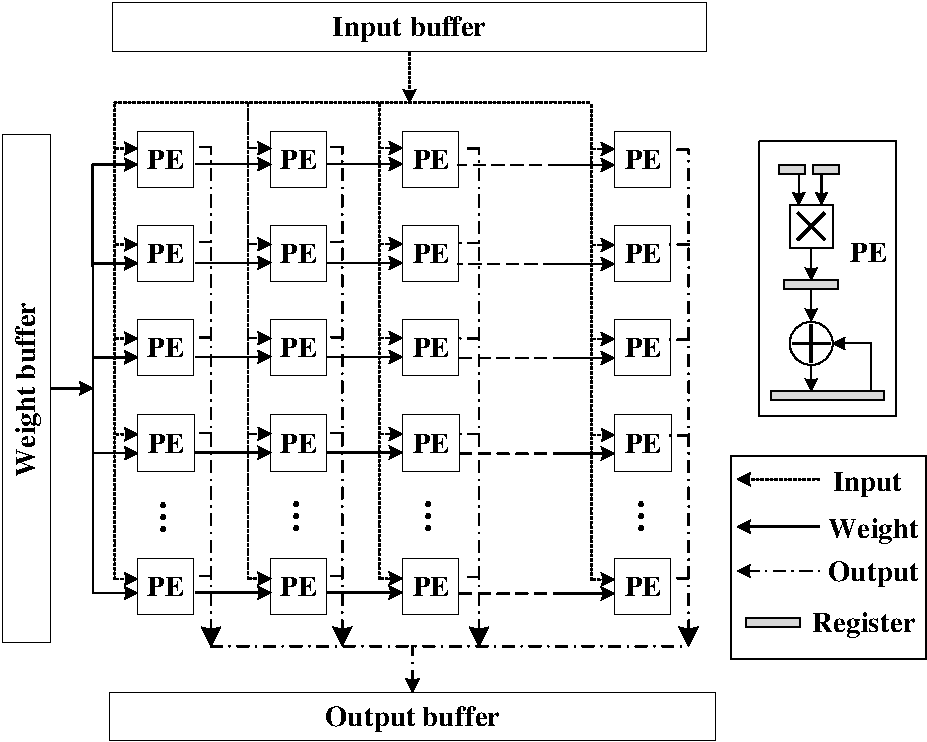
\includegraphics[width=0.7\linewidth]{images/HyCA-fig1.pdf}}
            \caption{A typical DLA with 2D computing array architecture.}
            \label{fig:accelerator}
            \vspace{-1em}
\end{figure}

\subsubsection{ ReRAM-based DNN Computing}

Deep neural network (DNN) is a  machine learning architecture which is composed of a series of computational layers and can be represented as a parametric function ${F}$:


\begin{equation} 
    F(x){\rm{ = }}{f_L}({W _L},{f_{L - 1}}({W _{L - 1}} \ldots ({f_0}({W _0},x))))
\end{equation} 
wherein ${x}$ represents the input and ${f_i}$ refers to the functional layers, including convolutional layers (CONV) and full connected layers (FC).

Nowadays, many specialized deep learning accelerators have been proposed to use ReRAM for edge neural network implementation at the \emph{inference process} \cite{7551380, 7920854}. ReRAM cells can not only work as on-chip memory, but also perform in-memory matrix-vector multiplication efficiently. As shown in Fig. \ref{fig:reramcomputing} (a), memristors are connected as a crossbar structure. When conducting a matrix multiplication $V \cdot G$,  the matrix $G$ is programmed as a set of  conductance values of the ReRAM cells, while the input vector is represented as a sequence of the analog word-line (WL) voltages $v_i$. When the voltages are applied to all the WLs simultaneously, the outputs of $V \cdot G$  are sensed as a current set $I$ automatically, achieving in-memory matrix multiplication effectively \cite{Liu:2019:FTN:3287624.3288743}. 

\begin{figure}
    \centering
    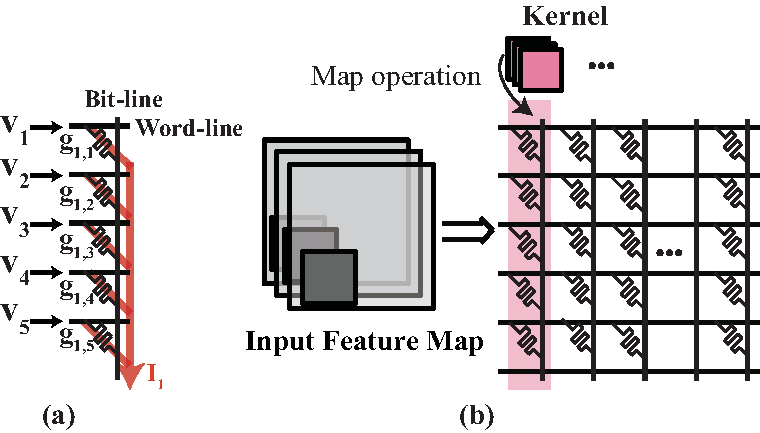
\includegraphics[width=0.9\linewidth]{images/OL-fig1}
    \caption{(a) The analog dot-product computing mechanism of ReRAM. (b) A simple mapping scheme of input feature maps and kernels.}
    \label{fig:reramcomputing}
    \vspace {-10pt}
\end{figure}

Ideally, the weight values are fixed after the training process. However, the unavoidable faults in the memristors will result in weight value fluctuation and further degrade the accuracy of DNN systems. Taking a CONV layer for an example, in each convolutional step, a multi-dimensional kernel slides over the input feature maps (IFMs)  to extract characteristics and produce the corresponding output feature maps (OFMs).  Fig. \ref{fig:reramcomputing} (b) illustrates a simple weight mapping scheme for convolutional layers. The parameters in the same kernel are reflected as the conductance of the ReRAM cells on a single bit-line. The IFMs are dot-multiplied by the kernel windows and represented as a series of input voltages, preparing to generate OFMs. It is worth pointing out that a specific convolutional kernel ${W}$ is fixed on the corresponding ReRAM cells and used to compute all output neurons in the corresponding OFM. As such, once a ReRAM cell becomes faulty, it will influence all the values of the corresponding OFMs and further propagate layer by layer, resulting in an erroneous output or even system failure \cite{Li:2017:UEP:3126908.3126964, xu2020hybrid, xu2021reliability}. 

{\bf SLC and MLC ReRAM.} Recently, many researches work on multi-level cell (MLC)-based deep learning accelerators rather than traditional single-level cell (SLC) devices. Unlike SLC memories, the MLC memories store a multi-bit value in a single ReRAM cell. However, there are trade-offs in MLC ReRAM memories. In an \emph{n}-level ReRAM MLC cell, the resistance state has to be encoded into \emph{n} levels. The stored values can be changed, even if the states of ReRAM cells have slightly drifted, which significantly increases the unreliability of ReRAM computation. Hence, many deep neural accelerators propose to represent one weight by multiple cells connected to the same WL. Each cell stores one or two bits rather than storing a whole weight in a single cell \cite{8715178}.  

\subsubsection{Neural Network Training Basis}
As shown in Fig. \ref{fig:networktraining}, a typical DNN training process consists of successive forward and backward propagations to evaluate current model's prediction accuracy and adjust its weights. During the forward step, the DNN is given with a set of input samples [$X,Y$] to compute the intermediate neurons [${a_0},{a_1}$] with weight matrices $W[{W_0},{W_1},{W_2}]$: 
\begin{equation}
    {a_{i + 1}} = {W_{i+1}}{a_i} + {b_{i+1}}
\end{equation}

wherein, $W_i$, $b_i$ is the weights and bias of layer $i$ respectively. Layers are connected with neurons. The output of layer $i$ is the input of the layer $i+1$. Then, the prediction error is calculated with the loss between final output  [${y_0},{y_1} \ldots {y_m}$] and the ground-truth label $Y$. To update the network parameters and minimize the prediction error, the loss $E$ is sent backward to all the prior layers and the weight matrix is updated as follows: 
\begin{equation}
    {W_i}{\rm{ = }} {W_i} - \eta \cdot \frac{{\partial E}}{{\partial {W_i}}}
    \label{eq:backforward}
\end{equation}
wherein, $\eta $ is the learning rate to control the  weight update speed. $E$ denotes the global error.  


During the iterative learning process, neural network itself will continue to adjust weight values to reduce the difference between the output prediction and the real label. Furthermore, this self-adjusting capacity of DNNs can also be used to retain faulty deep learning system's accuracy. Once there are unrepairable faults occurred in DLAs, weight values will be updated to adjust to these faults in the backward propagation process of each training iteration. However, using the traditional backward propagation algorithm (BP) consumes massive multiply-accumulate operations (MACs), which poses heavy computational pressure on resource-constrained edge devices. Hence, in this work, we modify the BP algorithm and propose a lightweight online model retraining mechanism to improve the convergence speed of the network training procedure and enable the faulty model to be retrained in-situ.

\begin{figure}
    \centering
    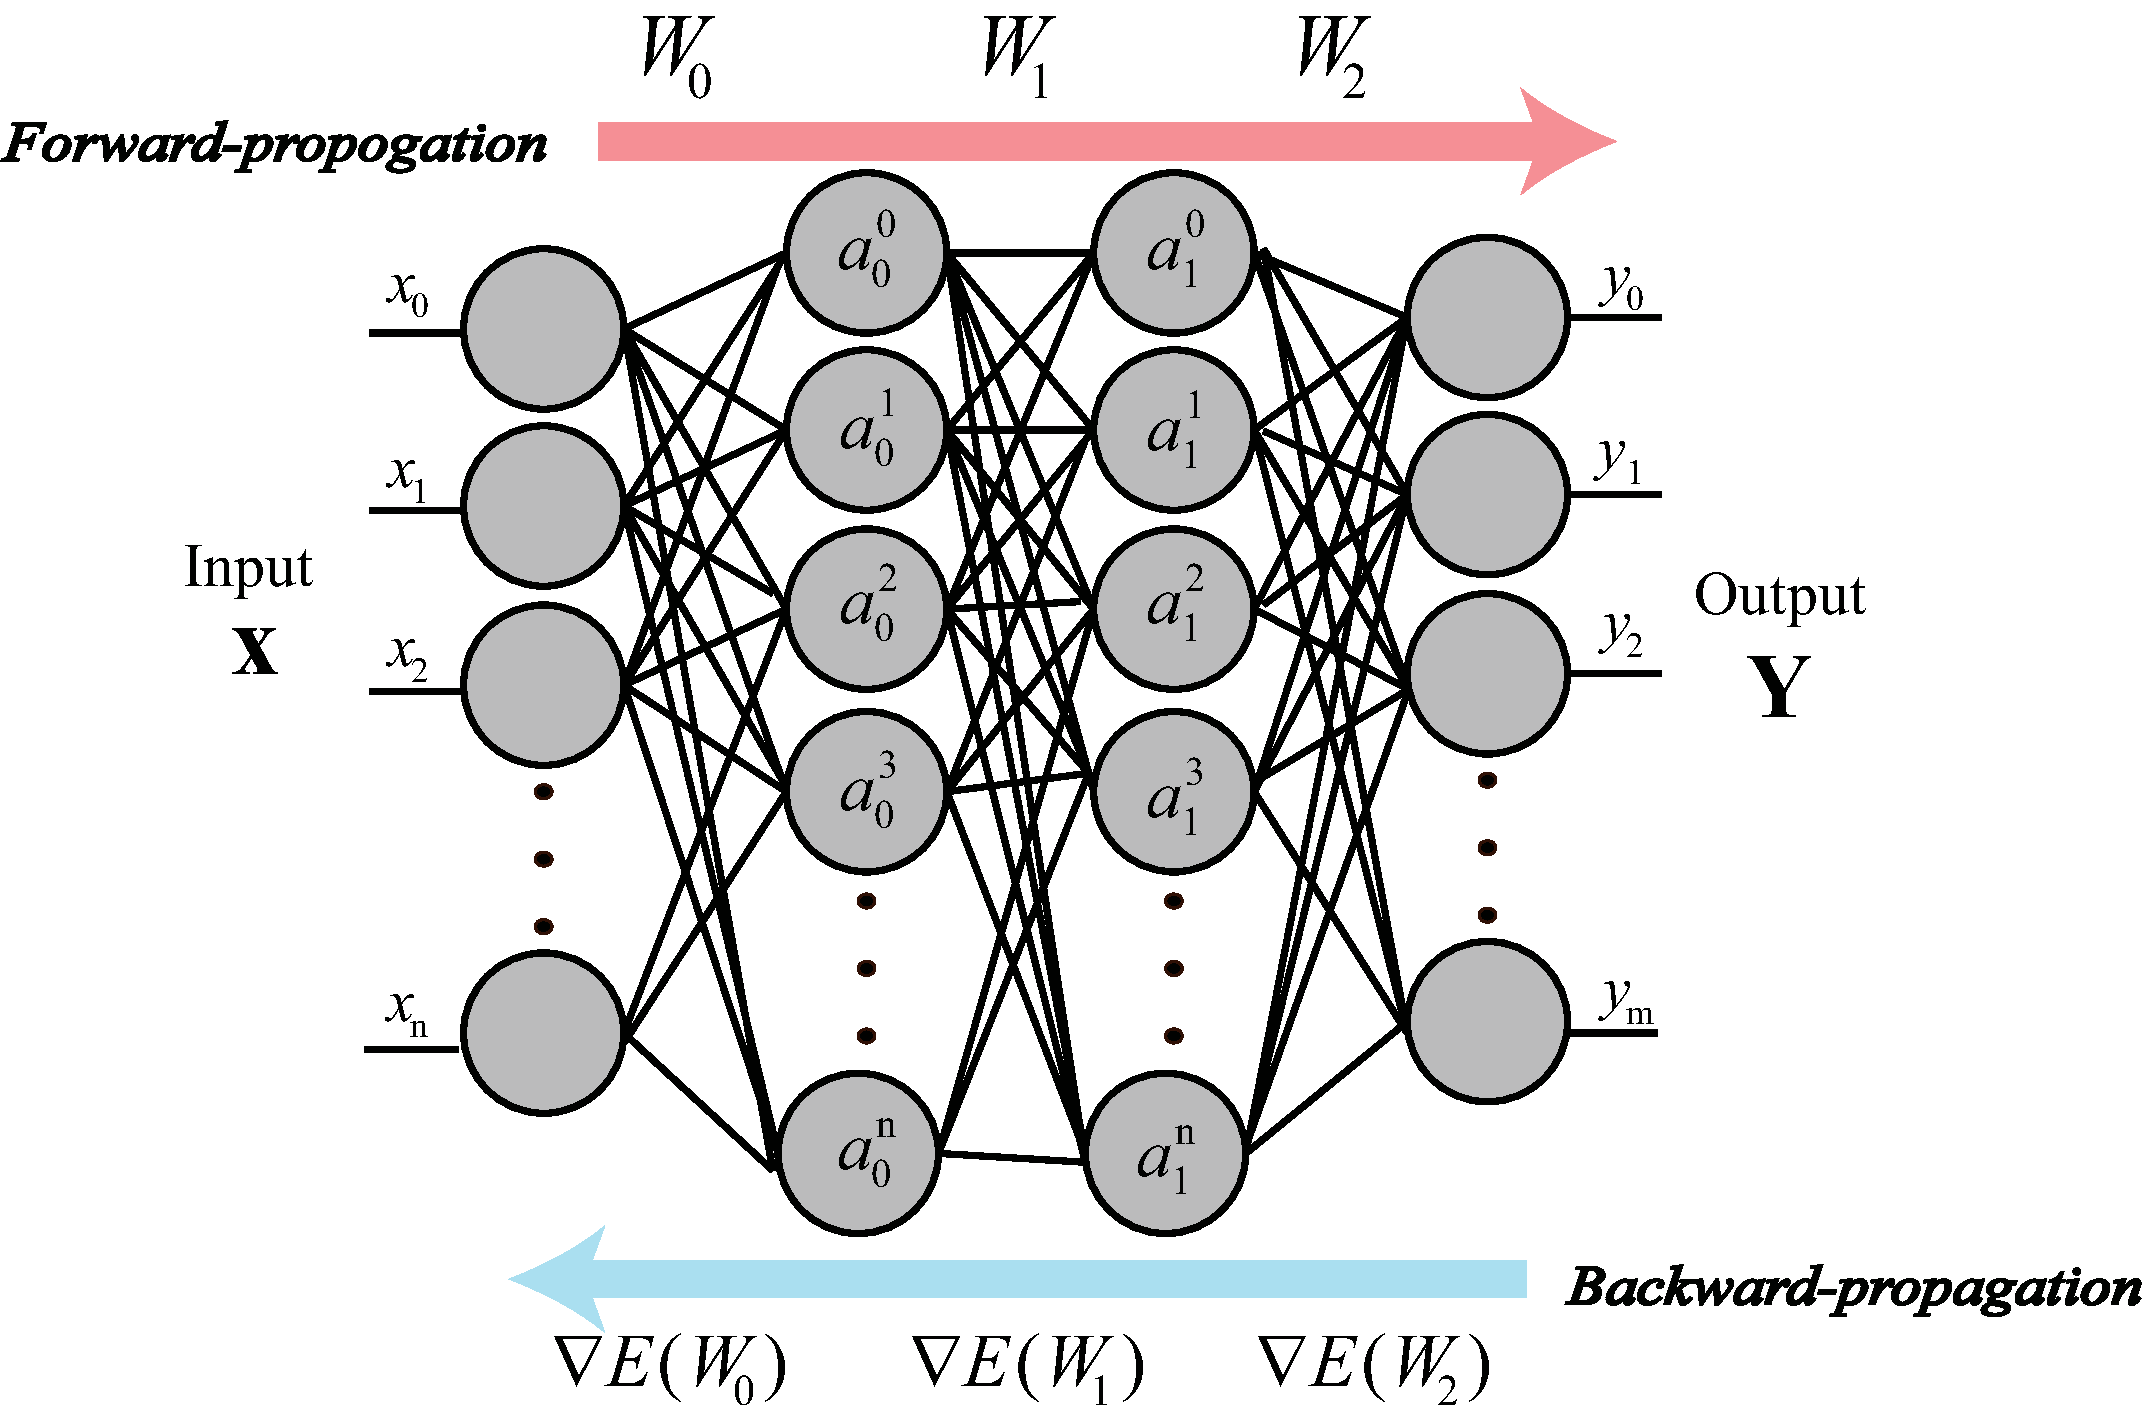
\includegraphics[width=1\linewidth]{images/OL-fig2}
    \caption{An illustration of the training process of a full-connected neural network.}
    \label{fig:networktraining}
    \vspace{-15pt}
\end{figure}

With the increasing adoption of deep learning in mission-critical applications, such as autonomous driving and drones, the reliability of DLAs widely utilized for the deep learning processing becomes critical and attracts a lot of attentions of the researchers recently \cite{mittal2020survey} \cite{xu2021reliability} \cite{xu2020persistent} \cite{ning2020ftt}. To analyze the influence of hardware faults on the deep neural network models, the authors in \cite{zhang2019fault} conducted comprehensive experiments and the experiment results show that hardware faults can lead to considerable prediction accuracy drop. For the TIMIT speech recognition task, the accuracy drops from 74.13$\%$ to 39.69$\%$. The accuracy loss is relevant to various design factors including the quantization, data format, and network architecture. It remains rather challenging to ensure resilient deep neural network execution on DLAs.

To alleviate the influence of hardware faults on neural network predictions, many prior works \cite{error2018date} \cite{energy2018kim} \cite{axtrain2018he} took advantage of the intrinsic fault-tolerance of neural network models by retraining the models for a specific fault configuration such that hardware faults can be compensated by the retrained models. Xu et al. \cite{xu2019resilient} proposed an on-accelerator retraining framework to obtain models that can tolerate the random hardware faults. Li et al. \cite{li2019squeezing} and Wang et al. \cite{wang2017resilience} proposed to employ the model retraining for DLAs with overclocking which may incur timing errors. To train resilient deep learning models, He et al. \cite{axtrain2018he} revised the loss function to obtain models that are less sensitive to the hardware faults. Unlike the above methods, Zhang et al. \cite{analyzing2018vts} \cite{zhang2019fault} proposed to bypass the faulty PEs in the computing array with zeros or other constant values such that the faults are more easier to tolerate via retraining. Although the retraining works for many fault configurations, there is still no guarantee that the retrained models can maintain the prediction accuracy for the target mission-critical applications because of the huge number of different fault configurations. In addition, the retraining can be rather expensive especially for large datasets and models, and is required for each specific fault configuration, which further limits the adoption of the retraining approaches. Unlike the retraining-based approaches, Hanif et al. \cite{abdullah2020salvagednn} proposed a training-free mapping approach to alleviate the influence of permanent PE faults in the DLA. It leverages the saliency of the neural network parameters and opts to map the salient weights to the faulty PEs as much as possible such that the negative influence of the PE faults on the neural network models is reduced. However, it works only when the fault error rate is low and can be sensitive to the fault distribution.  

To enable unmodified deep learning model execution without accuracy loss, an intuitive approach is to develop reliable DLA architectures with the conventional TMR and DMR approaches to tolerate the hardware faults, but these approaches incur substantial hardware resource consumption. In this case, the authors in \cite{takanami2017built}\cite{takanami2012built}\cite{horita2000fault} proposed to add redundant PEs to the large regular homogeneous computing array and each redundant PE can be shared by a group of PEs with distinct redundancy sharing methods such as row redundancy (RR), column redundancy (CR), and diagonal redundancy (DR). For the RR and CR, each row/column of the PEs share the same set of redundant PEs. For the DR, both the row and column of PEs corresponding to a diagonal location in the computing array share the same set of redundant PEs. Since the redundant PEs are shared by a group of homogeneous PEs, hardware resource consumption can be greatly reduced compared to DMR and TMR. Nevertheless, the faulty PEs may not be evenly distributed or even clustered across the computing array \cite{stapper1983integrated}. As a result, these approaches may fail to recover the computing array when the number of faulty PEs in each shared region such as a row or a column of PEs exceeds the the number of shared redundant PEs in the region. Thereby, the utilization of the redundant PEs can be affected by the fault distribution dramatically. More redundant PEs must be designed to ensure reliable execution. Otherwise, the performance can degrade dramatically when the faulty PEs are discarded due to the insufficient redundant PEs. Thereby, more efficient computing array architectures are required for the highly resilient DLA designs. 

On top of the redundancy-based fault-tolerant DLA designs, there are also many other different fault-tolerant architecture designs. The authors in \cite{ozen2019sanity} \cite{zhao2020algorithm} proposed a spatial and temporal checksum to protect full connection and convolution layers in deep neural network models. Zhang et al. \cite{zhang2020sorting} proposed a parallel stochastic computing(SC)-based neural network accelerator purely using bitstream computation by fully exploiting the superior fault tolerance of SC mainly for ternary neural networks. Li et al. \cite{li2020soft} proposed an error detecting scheme to locate incorrect PEs of the DLA and gave an error masking method to achieve fault-tolerance. Hamid Reza Mahdiani etc. \cite{mahdiani2012relaxed} proposed to relax the fault-tolerance of the VLSI implementation by employing TMR to only the computation of the most important bits such that the hardware overhead is reduced and the critical path latency is improved. Nevertheless, these approaches either require model retraining or can be sensitive to the fault distribution.


To address the reliability challenges in memristors, many hardware solutions have been proposed to tolerate permanent faults and soft faults. Error Correcting Code (ECC) has been studied in \cite{6165062} to alleviate the impact of process variations of memristors. However, this technique incurs high penalty with additional power and performance overhead. Besides, a squeeze-search method has been proposed in  \cite{6725492} to identify the ReRAM defects with a March algorithm directly. Though this approach is effective, its huge timing overhead prevents it from usage in on-line protection for edge devices. Besides, it brings in additional write operations, which further leads to memory wear-outs. Furthermore, remapping technology has also been explored. \cite{8119491} proposes to remap the model weights with redundant memristor columns. However, it still induces extra hardware waste.
                
Considering the huge costs of hardware-based methods, many software-based solutions have been devised recently. \cite{9045324} explores the network architecture search (NAS) algorithm to find reliable neural network architectures. However, this method only works for networks with skip connections. In \cite{7926952}, an offline training method has been proposed with a model mapping strategy. The authors used the prior knowledge of fault distributions to map the weight matrix to memristors and then conducted an offline model retraining to make memristors more resilient to faults by treating the faults as noises during training.  However, this method takes no consideration for the fault detection overhead. Moreover, the noise-tolerant models will still face accuracy degradation for some stuck-at faults and severe soft faults, because the training method can improve the robustness of the network model against faults but not completely eliminate the impacts of faults. 


\subsection{Challenges of Fault-Tolerant Deep Learning}
DLAs typically consist of a large regular computing array which can either be a systolic array or a plain mesh array\cite{jouppi2017datacenter, Chen2016Eyeriss}, and a set of on-chip buffers used for input features, output features, and weights. While the on-chip buffers implemented with SRAMs can be usually protected effectively with error correction code (ECC), we mainly focus on the reliability design of the regular computing array in this work. As each processing element (PE) in the computing array can be used for the calculation of multiple features in different network layers, faults in a single PE may cause multiple faulty computing results during the deep learning model execution. Thereby, they may result in considerable accuracy degradation according to our experiments in Section XXX. 

To mitigate the hardware faults in the 2-D computing array of DLAs, researchers have proposed a number of fault-tolerant design approaches from distinct angles. These approaches can be roughly divided into two categories. The first category mainly exploits the inherent fault-tolerance of the neural network models by retraining the neural network models specifically for the faulty computing array without any modification or with minor modification to the computing array \cite{deng2015retraining, zhang2019fault, xu2019resilient, li2019squeezing}. Although these approaches induce negligible hardware overhead and can even be applied to many off-the-shelf accelerators, the model retraining is required for each specific fault configuration, and the retraining, especially for large data sets and deep learning models, can be rather expensive. For instance, a critical neural network model applied in automotive systems must go through a series of standard certification tests before the modification can be accepted \cite{validation2019Ebert}. The cost of the certification test is nontrivial and time-consuming. Moreover, the prediction accuracy of the retrained models depends on both the model structures and the specific fault configurations. There is no guarantee that the model retraining can always maintain the original model accuracy and fulfill the requirements of mission-critical AI applications for all the different fault configurations by design.


To mitigate the hard faults and soft faults in ReRAM-based DNN accelerators, a number of approaches from distinct angles have been proposed. These approaches can be divided into the following categories. The first category is on-device training, which seeks to train a dedicated neural model to tolerate specific faults distributed on a memristor chip \cite{7167198}. It is particularly critical to address the unpredictable in-situ wear-outs and soft faults during the chip's life cycle. However, a straightforward on-device training that involves iterative back-propagation is usually expensive for the edge devices with limited computation capability and power budget. The second category is the traditional redundancy design with either software or hardware, which typically has the hardware components or the critical neurons/nodes replicated and has the computing results of the replicates voted to achieve resilient computing of the models \cite{5726731}. Nevertheless, it incurs considerable performance and energy overhead, which can easily violate the energy constraints of the typical edge devices. The third category is to conduct the on-line test and repair routinely in case of faults \cite{6725492}. A classical approach belonging to this category is `write-verify' and has been widely used for the memory blocks, but this scheme induces a large number of additional write operations, which will deteriorate the well-known wear-out problem of the memristors. As a result, when and how to perform the 'write-verify' to the ReRAM-based DNN accelerators without incurring wear-out remains a great challenge.

\section{Fault-Tolerant Deep Learning Architecture}
\subsection{Deep Learning Sensitivity to Hardware Faults}
The second category aims to recover the faulty computing array with redundant PEs. While the conventional approaches such as dual modular redundancy (DMR) and triple modular redundancy (TMR) require substantial hardware resources, researchers proposed a variety of relaxed redundancy approaches. The basic idea is to have each redundant PE to recover any faulty PE in a limited region of the computing array while the region can be a row, a column, or both row and column \cite{takanami2012built} \cite{takanami2017built}, which essentially limits the sharing of the redundant PEs and reduces the hardware resource consumption significantly compared to the DMR and TMR approaches. When the faulty PEs are evenly distributed across the computing array, the faulty PEs can be probably mitigated. Nevertheless, the faults may not be evenly distributed across the computing array and these approaches fail to recover the computing array even when the number of redundant PEs exceeds the number of the faulty PEs in the computing array. In this case, the DLAs will not be fully functional or degrade dramatically if the faulty PEs are discarded. In summary, there is still a lack of resilient computing array architectures for DLAs that allow unmodified deep learning model execution and can tolerate various fault distribution at the same time. 

To analyze the influence of hard errors on the above 2-D computing array, we inject random stuck-at bit errors to the registers of the PEs in a $32 \times 32$ computing array. We use bit error rate (BER) as the fault injection rate metric \cite{mittal2020survey}\cite{neggaz2018reliability}\cite{ares2018dac}, which refers to the total number of bit errors over the total bit number of the registers in the computing array. To facilitate the error characteristic of the 2-D computing array, we convert the BER to PE error rate (PER) instead. Both the input features and weights are 8-bit fixed point, so the input registers and the weight registers are set to be the same data width accordingly. The intermediate register in the PEs is set to be 16-bit and the accumulator in the PEs is set to be 32-bit in case of computing overflow. Thereby, there are 64 bit registers in total in each PE. While any persistent bit error in a PE is considered as an PE error, PER can be calculated using BER with ( Equation \ref{eq:error_rate}). Basically, it means that the PE is correct only when none of the bit registers are wrong. Otherwise, the PE will be faulty.

\begin{small}
    \begin{equation}
        \label{eq:error_rate}
        \begin{aligned}
                PER = 1-(1-BER)^{64}
        \end{aligned}
    \end{equation}
    \vspace{-1em}
\end{small}

We had random stuck-at bit errors injected to a DLA simulator implemented according to the architecture described in Figure \ref{fig:accelerator} for the fault analysis. We took Resnet18 pre-trained on ImageNet \cite{deng2009imagenet} as an example and had it implemented on the accelerator with random faults. In this case, we generated 50 random fault configurations and evaluated the prediction accuracy under different PER setups. The experiment result is shown in Figure \ref{fig:bit}. It reveals that the prediction accuracy varies dramatically across the different fault configurations. When the PER is higher than 1\%, the prediction accuracy of the model mostly degrades to zero. Moreover, we notice that the prediction accuracy may also drop considerably in some of the fault configurations even under very low PER. It indicates that the model accuracy depends on not only the PER but also the fault distribution. Thereby, protecting the computing array is required for mission-critical applications despite the fault injection rate. 

\begin{figure}
    \setlength{\abovecaptionskip}{-1pt}
    \setlength{\belowcaptionskip}{0pt}
        \center{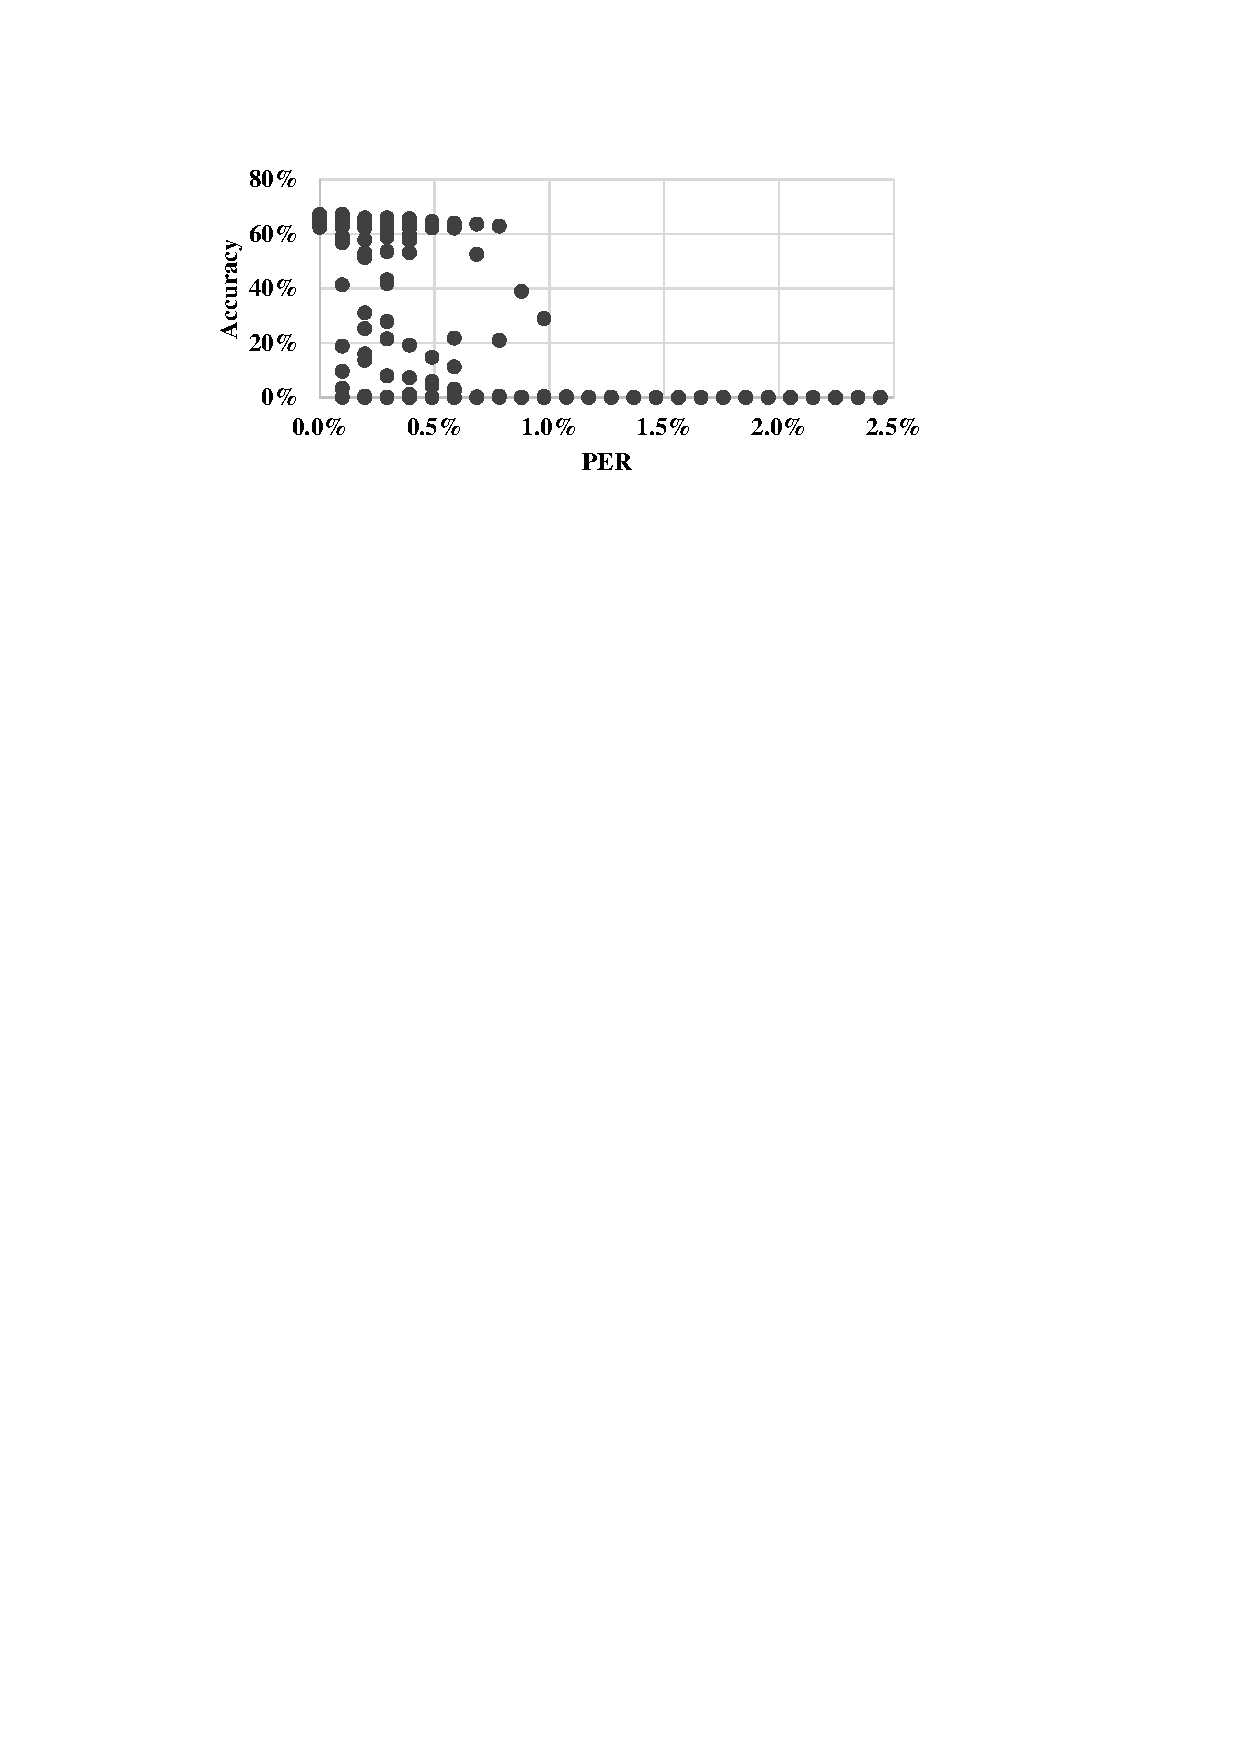
\includegraphics[width=0.7\linewidth]{images/HyCA-fig2.pdf}}
            \caption{Prediction accuracy of Resenet18 executed on a typical DLA under different PER setups. For each PER setup, 50 random fault configurations are evaluated on ImageNet.}
            \label{fig:bit}
\end{figure}

\begin{figure}
    \setlength{\abovecaptionskip}{-1pt}
    \setlength{\belowcaptionskip}{0pt}
        \center{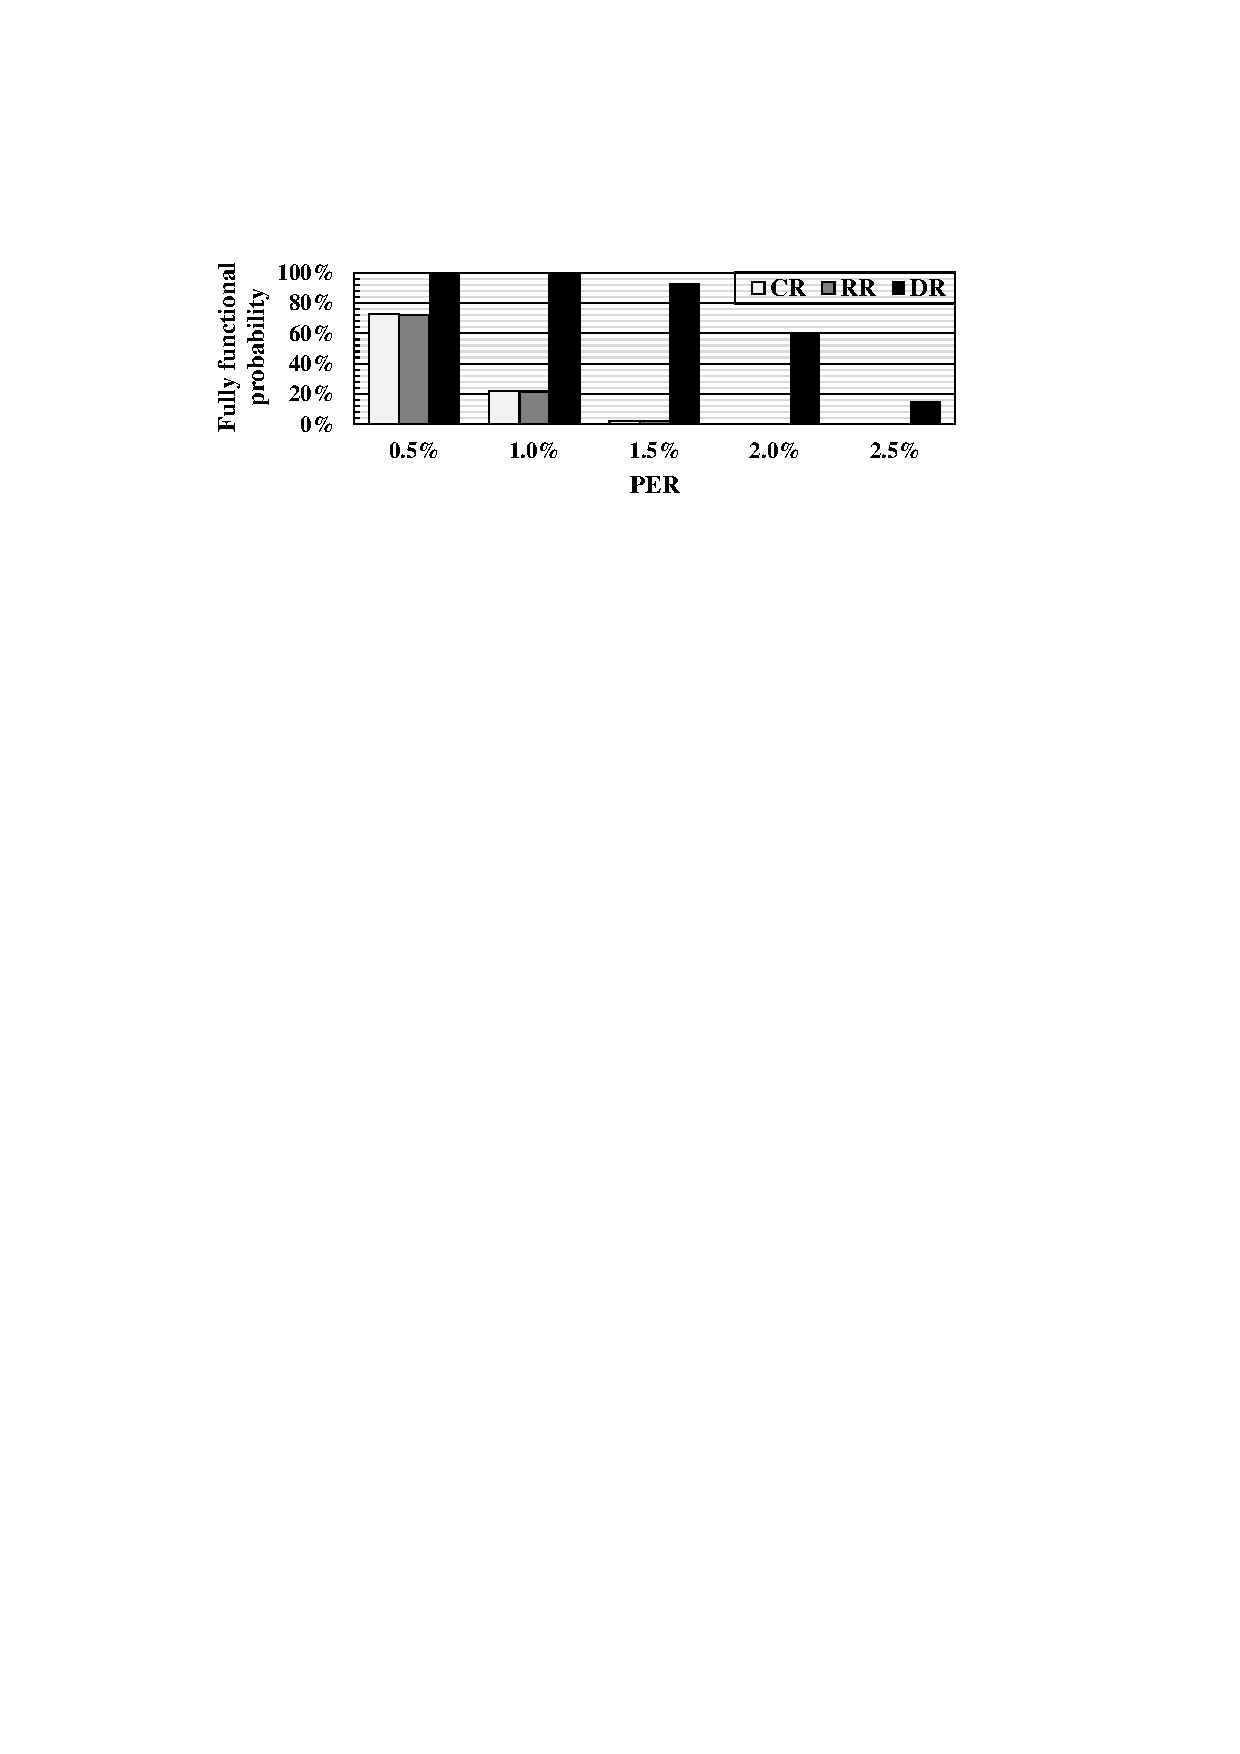
\includegraphics[width=0.7\linewidth]{images/HyCA-fig3.pdf}}
            \caption{The fully functional probability of the 2-D computing array under different PER setups.}
            \label{fig:mo}
            \vspace{-1em}
\end{figure}

In addition, we further evaluated the classical hardware redundancy strategies, i.e. RR, CR, and DR for the regular 2-D computing array and measured the fully functional probability of the computing array under different PER setups. The evaluation result is shown in Figure \ref{fig:mo}. It can be observed that these classical redundant design approaches can hardly mitigate all the faulty PEs even when the PER is around 1\% which indicates that there are only 10 faulty PEs on average. In contrast, the number of redundant PEs is 32, which is much larger than the number of faulty PEs. It demonstrates that the redundant PEs cannot be fully utilized by these redundancy strategies because of the unevenly faulty PE distribution. The situation further deteriorates with the increase of the PER, which can be rather risky for the mission-critical AI applications.


\subsection{Recomputing Based Hybrid Computing Architecture}
In this section, we will present an overview of the proposed hybrid computing architecture (HyCA) for fault-tolerant DLAs first. Then, we will illustrate the dataflow for the fault mitigation, HyCA microarchitecture, and fault detection with HyCA respectively.

\textbf{HyCA Overall Architecture:}
In order to tolerate various fault configurations with a unified computing architecture, we propose a hybrid computing architecture (HyCA), which has a dot-production processing unit (DPPU) seated along with the regular 2-D computing computing array, to recompute all the operations mapped to the faulty PEs in arbitrary locations of the computing array as shown in Figure \ref{fig:mapping}. While the 2-D computing array has each PE to calculate the different output features sequentially given the output stationary dataflow \cite{Chen2016Eyeriss} and the DPPU has all the PEs to compute a single output features in parallel, they have distinct read patterns of the input features and weights from the corresponding on-chip buffers. More specifically, the 2-D computing array needs to read an array of input features in the same row and channel in each cycle while DPPU needs to read an array of input features aligned in channel dimension in each cycle. Thereby, the on-chip buffers cannot fulfill the read operations of the two computing units at the same time due to the limited read ports and distinct data layout requirements. To make sure that the normal 2-D array processing will not be affected by the DPPU recomputing, the on-chip buffer design remains unchanged. In this case, DPPU cannot read the required weights and input features aligned in channel dimension if it starts the recomputing at the same time with the 2-D computing array. 

\begin{figure}
    \setlength{\abovecaptionskip}{-2pt}
    \setlength{\belowcaptionskip}{0pt}
        \center{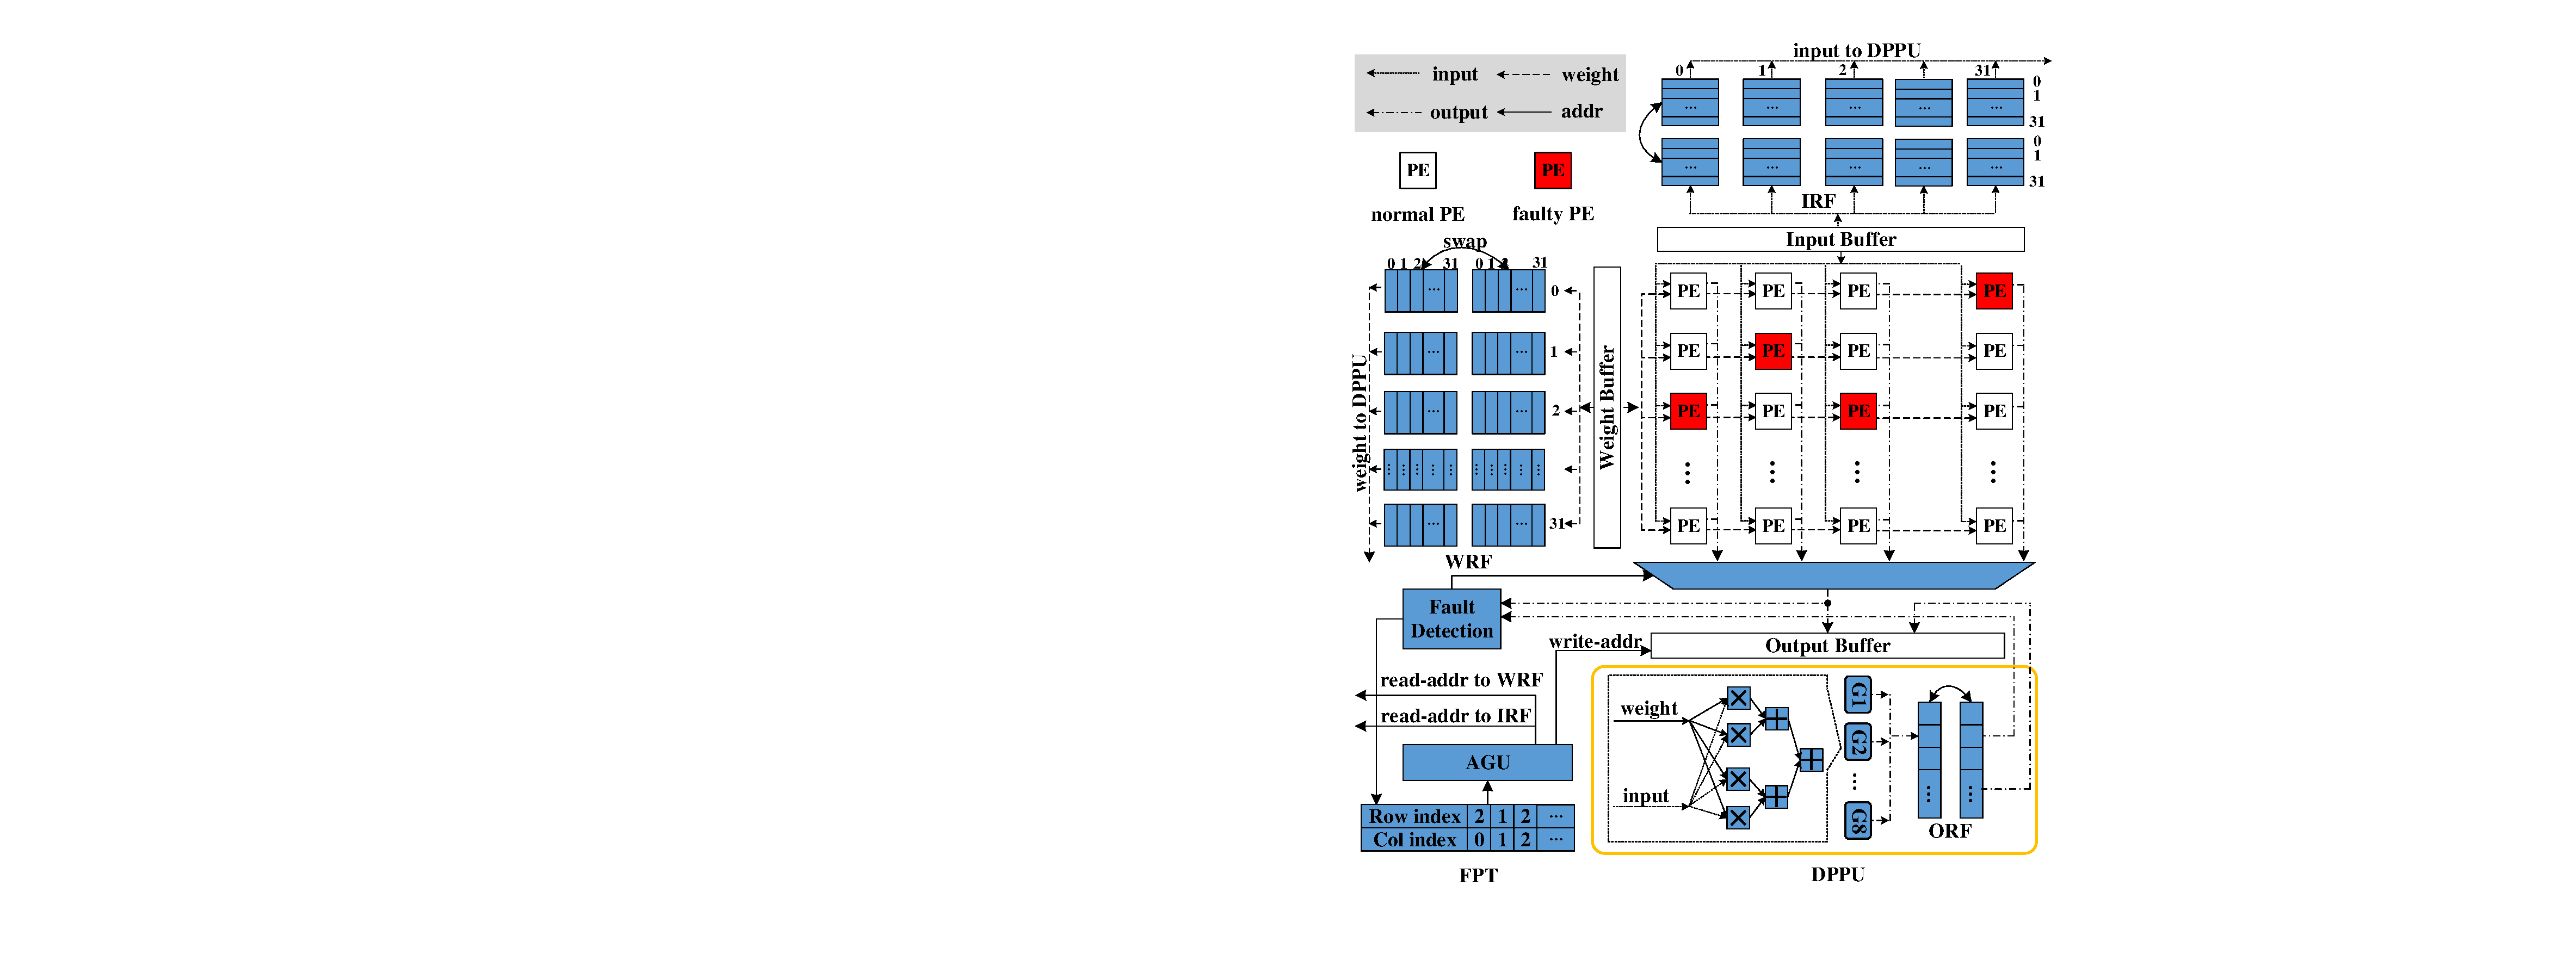
\includegraphics[width=0.7\linewidth]{images/HyCA-fig4.pdf}}
            \caption{Overview of of a DLA with Hybrid Computing Architecture. The components highlighted with blue are added to the conventional DLA to tolerate faulty PEs in arbitrary locations of the 2-D computing array.}
            \label{fig:mapping}
            \vspace{-1.5em}
\end{figure}

\begin{figure*}[tb]
    %\setlength{\abovecaptionskip}{-2pt}
    \setlength{\belowcaptionskip}{0pt}
        \center{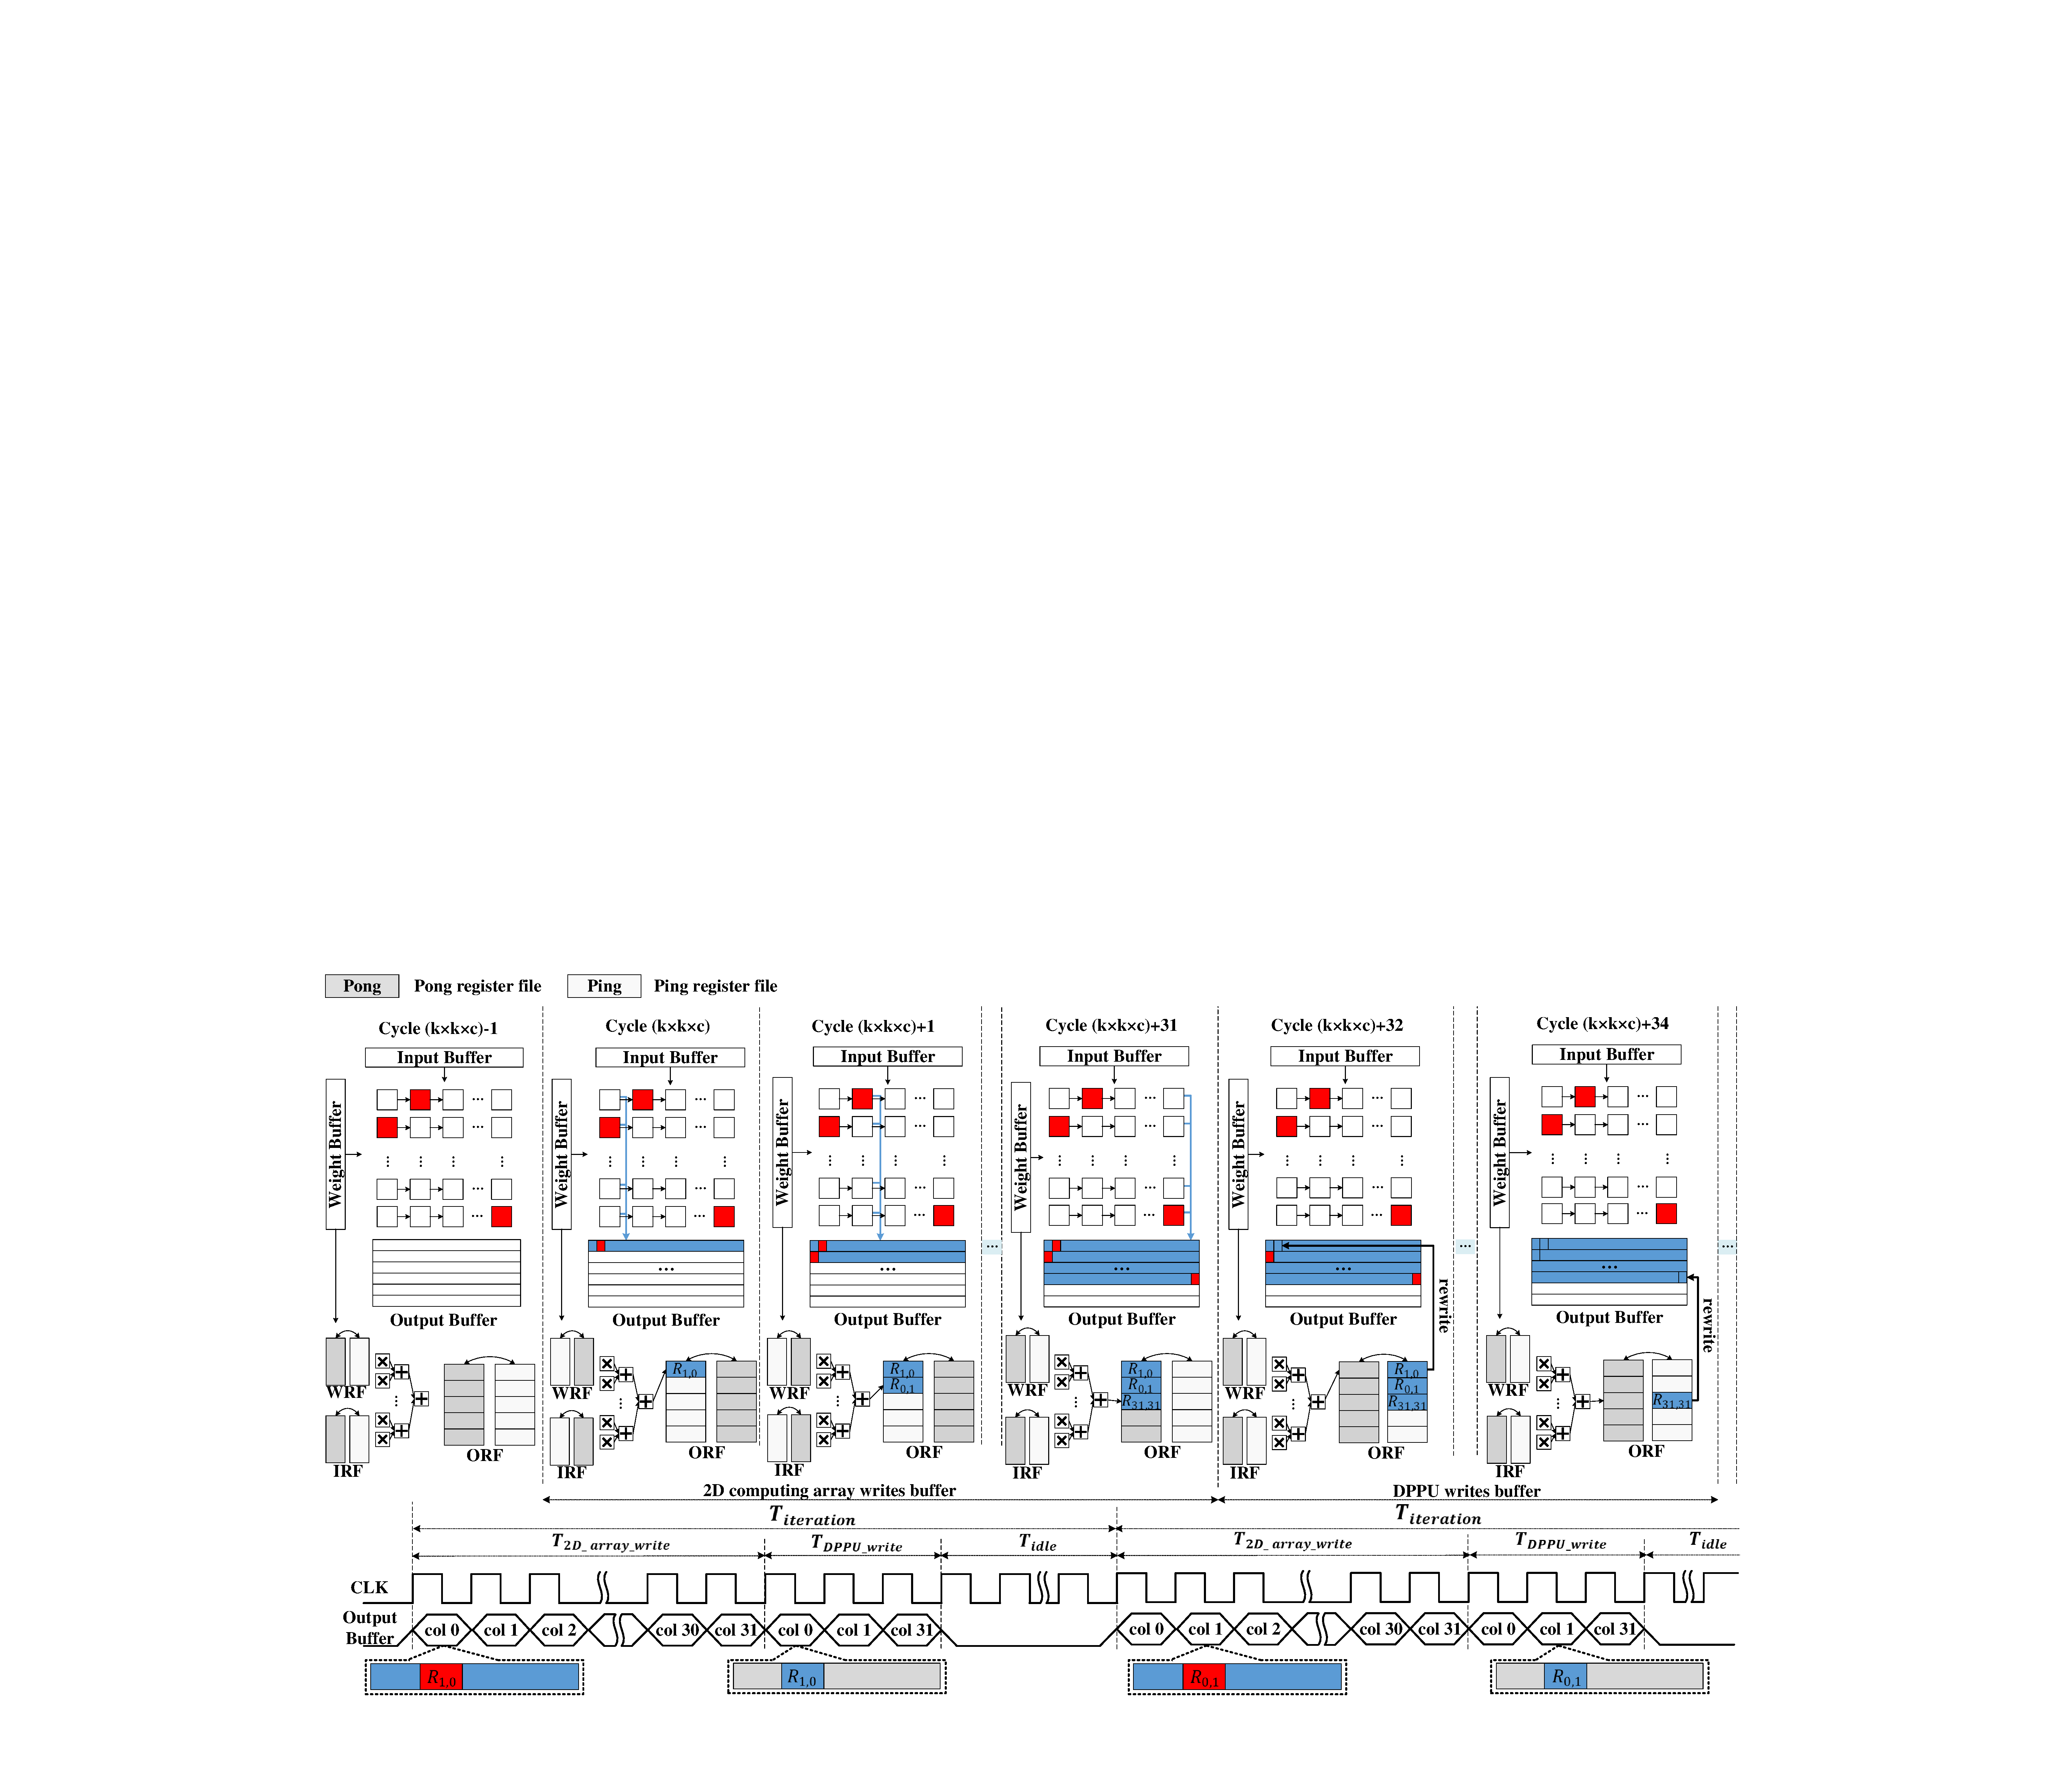
\includegraphics[width=1\linewidth]{images/HyCA-fig5.pdf}}
            \caption{The dataflow of using DPPU for recomputing the neural network operations mapped on the faulty PEs of a typical DLA. It also demonstrates how the DPPU overwrites the faulty computing results produced by the 2-D computing array.}
            \label{fig:pipeline}
            \vspace{-1em}
\end{figure*}

To address the problem, we have the input features and weights buffered in an input register file (IRF) and a weight register file (WRF) respectively while they are read for the 2-D computing array processing. Meanwhile, we have the recomputing delayed until there are sufficient inputs and weights ready for the recomputing. Accordingly, the delay must be larger than or equal to the number of weights required by DPPU data consumption in a single cycle to ensure DPPU can be fully utilized. As the DPPU may recompute operations on any PE in the 2-D computing array, the delay also needs to be larger than or equal to $Col$ when the last column of the PEs obtain the weights passed from the first column of PEs. Suppose $D$ represents the delay, then $D \geq Col$. Note that $Col$ refers to the column size of the 2-D computing array. In this work, we organize IRF and WRF in Ping-Pong manner to ensure that the 2-D computing array can continue the normal dataflow without any stall during the DPPU recomputing. As the DPPU conducts the output feature calculation in parallel, DPPU can always finish the recomputing of the operations mapped to the faulty PEs before the Ping-Pong register files swap with each other when the DPPU size does not exceed the number of the faulty PEs. Note that DPPU size refers to the number of multipliers in DPPU. Since the peak computing power of DPPU equals to that of the 2-D computing array when configured with the same number of PEs, DPPU size is comparable to the 2-D computing array size and can also be used to represent its computing power. This also explains why DPPU can always finish the recomputing tasks before new weights and inputs are ready when DPPU size is larger than the number of faulty PEs in the 2-D computing array. 

In addition, we have a fault PE table (FPT) to record the coordinates of the faulty PEs in the 2-D computing array which can be usually obtained with a power-on self-test procedure. With the coordinates, an address generation unit (AGU) is used to generate the read addresses and instruct the DPPU to read the right input features and weights from the register files. Moreover, AGU also determines the addresses to the output buffer for the overlapped writes of the recomputed output features. Similar to the IRF and WRF, there is also a Ping-Pong register file called ORF for the DPPU outputs and it is utilized to pipeline the DPPU recomputing and the write from DPPU to the output buffer.

While DPPU can be utilized to calculate any output features mapped to the 2-D computing array, we can also use DPPU to check whether the calculation of an output feature in the 2-D computing array is correct, which can be used to detect the wear-out or aging induced persistent errors at runtime. If the computing results obtained from the 2-D computing array and DPPU do not match, it indicates that the corresponding PE in the 2-D computing array is faulty as DPPU with much smaller sizes compared to the 2-D computing array can be easily protected with much less overhead and is usually considered to be correct. By changing the fault PE table and scanning the computing of all the PEs in the 2-D computing array sequentially, we can detect the PE faults at runtime without affecting the 2-D computing array processing. Basically, the redundant recomputing mechanism can be mostly reused by the fault detection. And we only need a tiny fault detection module to conduct the scanning of the 2-D computing array and the comparison to the DPPU processing. Details of the fault detection module will be illustrated in the rest of this section.

\textbf{HyCA Dataflow for Fault Mitigation}
To further illustrate the dataflow in HyCA especially the redundant computing unit DPPU, we take HyCA with a $32 \times 32$ 2-D computing array and three faulty PEs as an example. DPPU in the HyCA has 32 PEs included. The example is shown in Figure \ref{fig:pipeline}. Suppose $c$ and $k$ represent the input channel depth and the convolution kernel size respectively. It takes a PE in the 2-D computing array $k \times k \times c$ cycles to produce a convolution output. Without loss of generality, assume that the example starts at Cycle $k \times k \times c - 1$ when the first column of PEs complete a set of output feature calculation. The 2-D computing array occupies the output buffer until the last column of PEs complete the output feature data. Afterwards, the 2-D computing array may start to compute the new output features, but it usually takes $k \times k \times k \times c$ cycles to complete with the output stationary dataflow. In this case, DPPU starts to use the output buffer and update the recomputed results to the output buffer without write conflicts. The processing steps are detailed as follows.

\begin{enumerate}
    \item At cycle $k\times k\times c - 1$, the first column of PEs produce a column of output features accordingly and pass the weights to the second column of PEs. At the same time, the weights and input features used in the first column of PEs are stored in the corresponding Pong register file.

    \item At cycle $ k\times k\times c $, the first column of PEs write the calculated output features to the output buffer and start the calculation of new output features. Since PE(1,0) is faulty, the computing result written to the output buffer from this PE as marked with red color was wrong. While the input features and weights that are used for the output feature calculation on PE(1, 0) remain stored in the IRF and the WRF respectively, they will be read to the DPPU for the recomputing at this cycle. 

    \item At cycle $ k\times k\times c + 31$, the Pong WRF and the Pong IRF are filled with the newly incoming weights and inputs, and they will be kept for 32 cycles. Weights and input features coming in next cycle will overwrite the data in the Ping WRF and the Ping IRF respectively. Thereby, DPPU must finish the recomputing that depends on the weights stored in the Ping WRF and IRF at this cycle. Otherwise, the data in the Ping register files will be overwritten. Afterwards, the processing repeats from the first processing step for another 32 cycles until the end of the convolution calculation.

    \item At cycle $ k\times k\times c + 32$, DPPU has the recomputed output features in the output register file (ORF) written to the output buffer with a byte mask such that only the recomputed output feature is updated. Meanwhile, it starts to recompute the latest set of output features that are mapped to the faulty PEs in the 2-D computing array. As each output feature calculation is mapped to a single PE in the 2-D computing array using the classical output stationary dataflow, it takes $c \times k \times k$ cycles to complete an output feature calculation. As $c \times k \times k$ is usually larger than 32, and the output buffer will be occupied for only 32 cycles during each set of output feature calculation, the recomputed output feature data can be updated to the output feature buffer without conflicts. %In addition, DPPU can also conduct the partial convolution in parallel with the 2-D computing array and it needs to store the partial convolution results in output registers until the entire recomputed features are obtained, so we also have DPPU equipped with Ping-Pong output registers. 

    \item At cycle $ k\times k\times c + 34$, because there are only three faulty PEs in the 2-D computing array, it takes the DPPU three cycles to have the recomputed results overwritten from the ORF to the output buffer.

    \item From cycle $ k\times k\times c + 35$ to $ k\times k\times c + c$, both the 2-D computing array and the DPPU conduct the partial convolution locally, so the output buffer port is idle before the first column of PEs complete the new output feature calculation. 

\end{enumerate}

As shown in Figure \ref{fig:pipeline}, the overall processing is conducted iteratively. Each iteration includes a set of complete output feature calculation and it can be divided into three phases, i.e. 2-D array write, DPPU write, and idle from the perspective of the output buffer status. While each PE produces an output feature data per iteration and a PE conducts one MAC per cycle, the processing time of an iteration is $T_{iteration}=c \times k \times k$. For the 2-D computing array write, it takes $T_{2D\_arrary\_write} = D$ cycles per iteration where $D$ refers to the number of cycles that DPPU delays after the 2-D computing array processing. For the DPPU write, it needs $T_{DPPU\_write}=fault\_PE\_num$ cycles as the DPPU updates the recomputed output features sequentially. However, DPPU recomputing does not have to start after the entire computing of the output features on the 2-D computing array. Instead, it is pipelined with the 2-D computing array but only $D$ cycles slower. Thus, the weights and the input features consumed by the 2-D computing array must be fully accommodated by the Ping-Pong register files during the $D$ cycles. Accordingly, the depth of weight and input feature Ping-Pong register files is set to be $2\times D \times Row$. To minimize the register file overhead, we set $D=Col$.

As the average throughput of a PE in the 2-D computing array is the same with that in the DPPU, each multiplier in the DPPU can be used to repair a faulty PE in the 2-D computing array. Thereby, the DPPU size essentially represents the capability of the fault tolerance of the proposed HyCA without performance penalty. When the number of faulty PEs is larger than the DPPU size, we seek to preserve the computing power as much as possible without altering the target neural network models. To that end, we discard the faulty PEs that cannot be repaired due to the lack of the computing redundancy in the DPPU. As it is usually inefficient to compile and deploy the neural network models to a computing array with irregular row sizes which can cause both the irregular on-chip buffer accesses and external memory accesses, we choose to discard the columns with unrepaired faulty PEs and the columns that are disconnected from the input/weight/output buffers. Moreover, HyCA can repair any faulty PEs in the 2-D computing array, so it offers more flexibility to prioritize the faulty PEs for repairing such that the surviving computing array can be maximized especially when there are insufficient redundant PEs. In this work, the maximum remaining computing array can be obtained simply by assigning higher repairing priority to the faulty PEs on the left, which ensures that the surviving computing array is connected to the on-chip buffers. 

\subsection{HyCA Micro-architecture}
In this section, we will illustrate the major components of HyCA added to the baseline DLA and they include the DPPU, register files, and the fault PE table (FPT). FPT keeps the coordinates of the faulty PEs that will be repaired by the DPPU. As the maximum number of faulty PEs that can be tolerated without performance penalty is determined by the DPPU size, FPT is configured with $DPU\_size$ entries accordingly. Address generation unit (AGU) is a piece of control logic that generates the access addresses of the weight register file, input register file, and output register file based on the FPT for the recomputing of the DPPU. The structures of FPT and AGU are simple and we will not dwell on it. In contrast, the DPPU and the register files are relatively more complex, and they dominate the hardware overhead. Thus, they will be detailed in the rest of this section.

\begin{figure}
    \setlength{\abovecaptionskip}{-10pt}
    \setlength{\belowcaptionskip}{0pt}
        \center{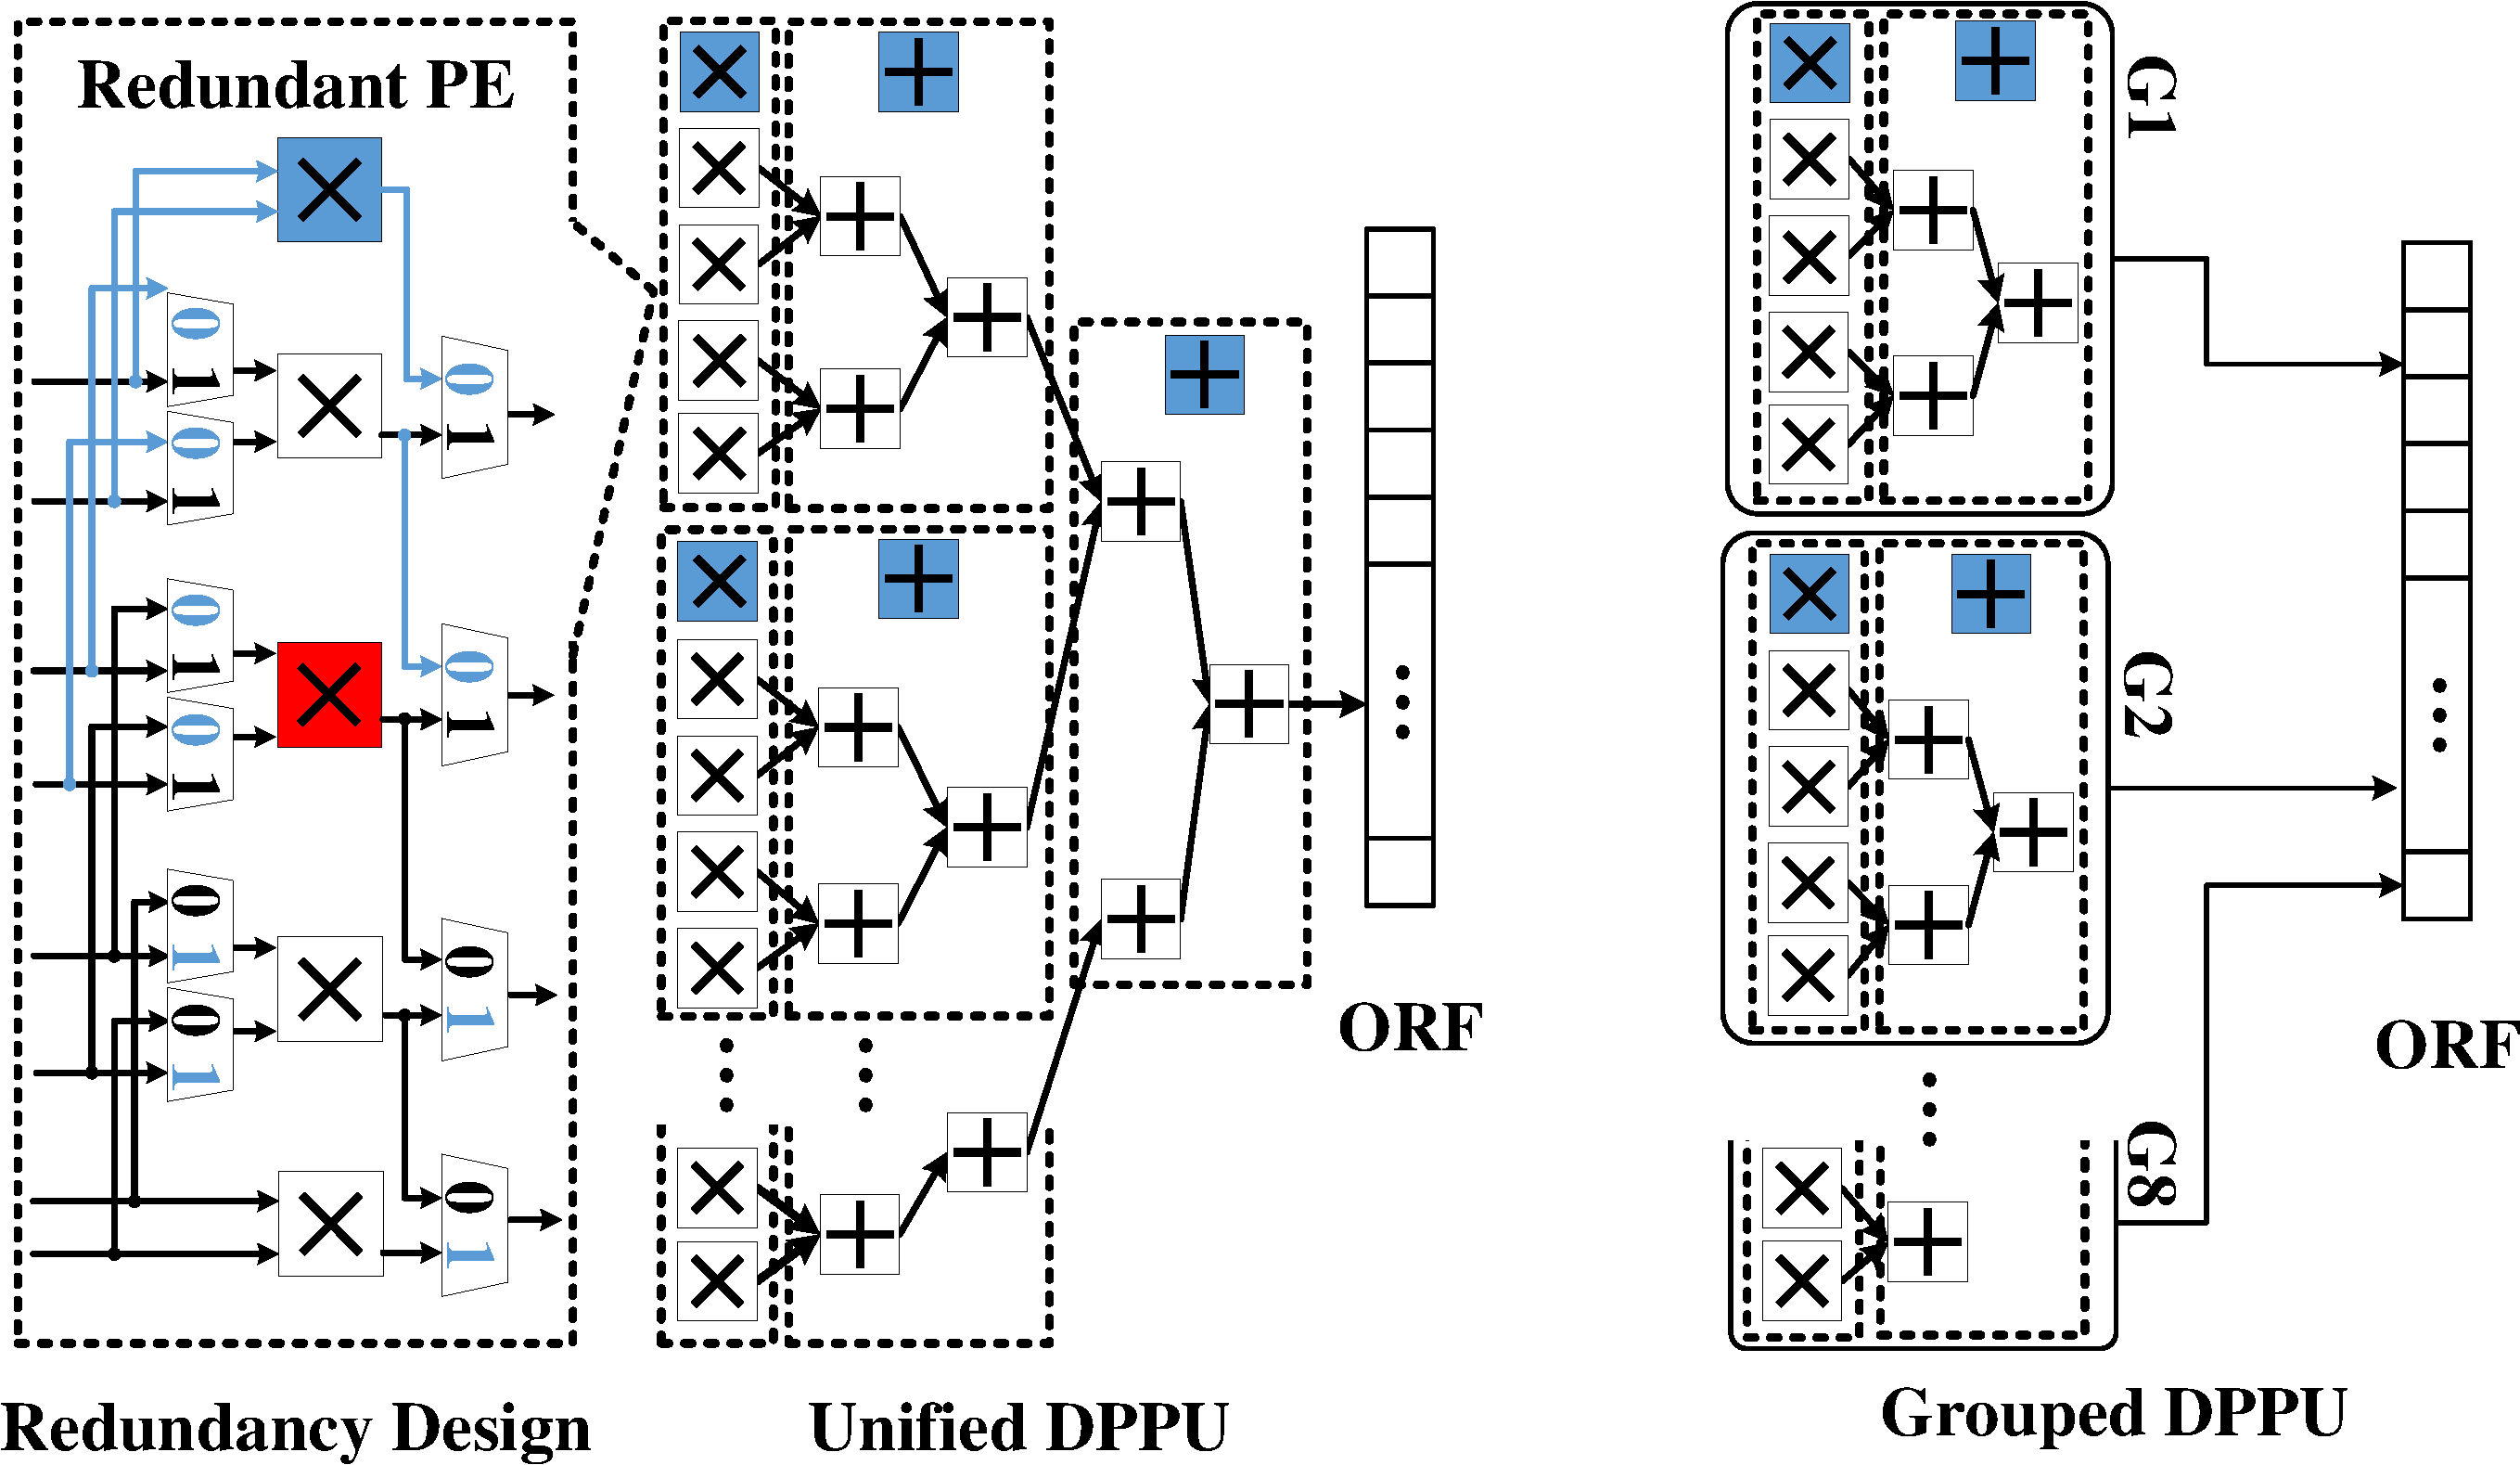
\includegraphics[width=0.8\linewidth]{images/HyCA-fig6.pdf}}
            \caption{Structures of the unified DPPU and the grouped DPPU. For both the unified DPPU and the grouped DPPU, they are protected with redundant PEs. Each redundant PE is used to protect a set of homogeneous PEs and these PEs are connected with ring topology to reduce the signal fan-out.}
            \label{fig:deg}
            \vspace{-1em}
\end{figure}

\textbf{Dot-Production Processing Unit (DPPU)}

DPPU is utilized for the dot-production and it consists of a set of multipliers as well as an adder tree that is used to aggregate all the multiplication results in a pipelined manner. It is mainly used to recompute the output features that are mapped to the faulty PEs in the 2-D computing array. An intuitive implementation is to construct a single unified dot-production unit which has both the input features and weights read from the corresponding register files in a single cycle and processed in parallel. As DPPU starts $Col$ cycles later after the 2-D computing array, each faulty PE in the 2-D computing array has $Col$ weights and input features multiplied and accumulated. Accordingly, $Col$ weights and input features can be extracted for the recomputing on DPPU for each faulty PE in the 2-D computing array. In order to make best use of the PEs in the DPPU, the $Col$ weights and input features must be fully distributed to the DPPU. If the entire DPPU is organized into a unified dot-production unit, the size of the DPPU is rather limited, which hinders the scalability of the DPPU. For instance, when $Col$ is set to be 32 and DPPU size is set to be 24 or 48, the computing mapped to a single faulty PE cannot be perfectly mapped to the DPPU, which will lead to the under-utilization of the DPPU. To address this problem, we propose to divide the PEs in the DPPU into multiple smaller groups and each group can conduct the dot-production independently. As the number of PEs in each group gets smaller, they are more likely to be fully utilized by the computing mapped to a faulty PE. As shown in Figure \ref{fig:deg}, each group includes 8 PEs and it completes the computing of a faulty PE in 4 cycles when $Col$ is set to be 32. In this case, the DPPU size can be scaled conveniently. At the same time, the different groups can conduct operations mapped to different faulty PEs in the 2-D computing array in parallel.  

While the DPPU is used to recompute all the faulty operations in the 2-D computing array, it must be resilient enough to ensure the functionality. Otherwise, a single fault in the DPPU may corrupt the whole accelerator. To improve the resilience of the DPPU, we add redundant PEs to the DPPU as shown in Figure \ref{fig:deg}. Basically, the multipliers used in the DPPU are divided into groups and each group is equipped with a redundant multiplier. Instead of having the redundant multiplier shared by all the multipliers in the group, we have the redundant multiplier and the multipliers in the group connected in a directed ring topology and each multiplier can be configured to replace its downstream neighboring multiplier. When any of the multiplier fails, it can be replaced by its upstream multiplier immediately. Compared to the shared redundancy design, this approach can avoid high fan-out connections to the redundant multipliers. Similarly, we also have the adders in the adder tree protected with the same redundancy design approach. 

\begin{figure}
    \setlength{\abovecaptionskip}{0pt}
    \setlength{\belowcaptionskip}{0pt}
        \center{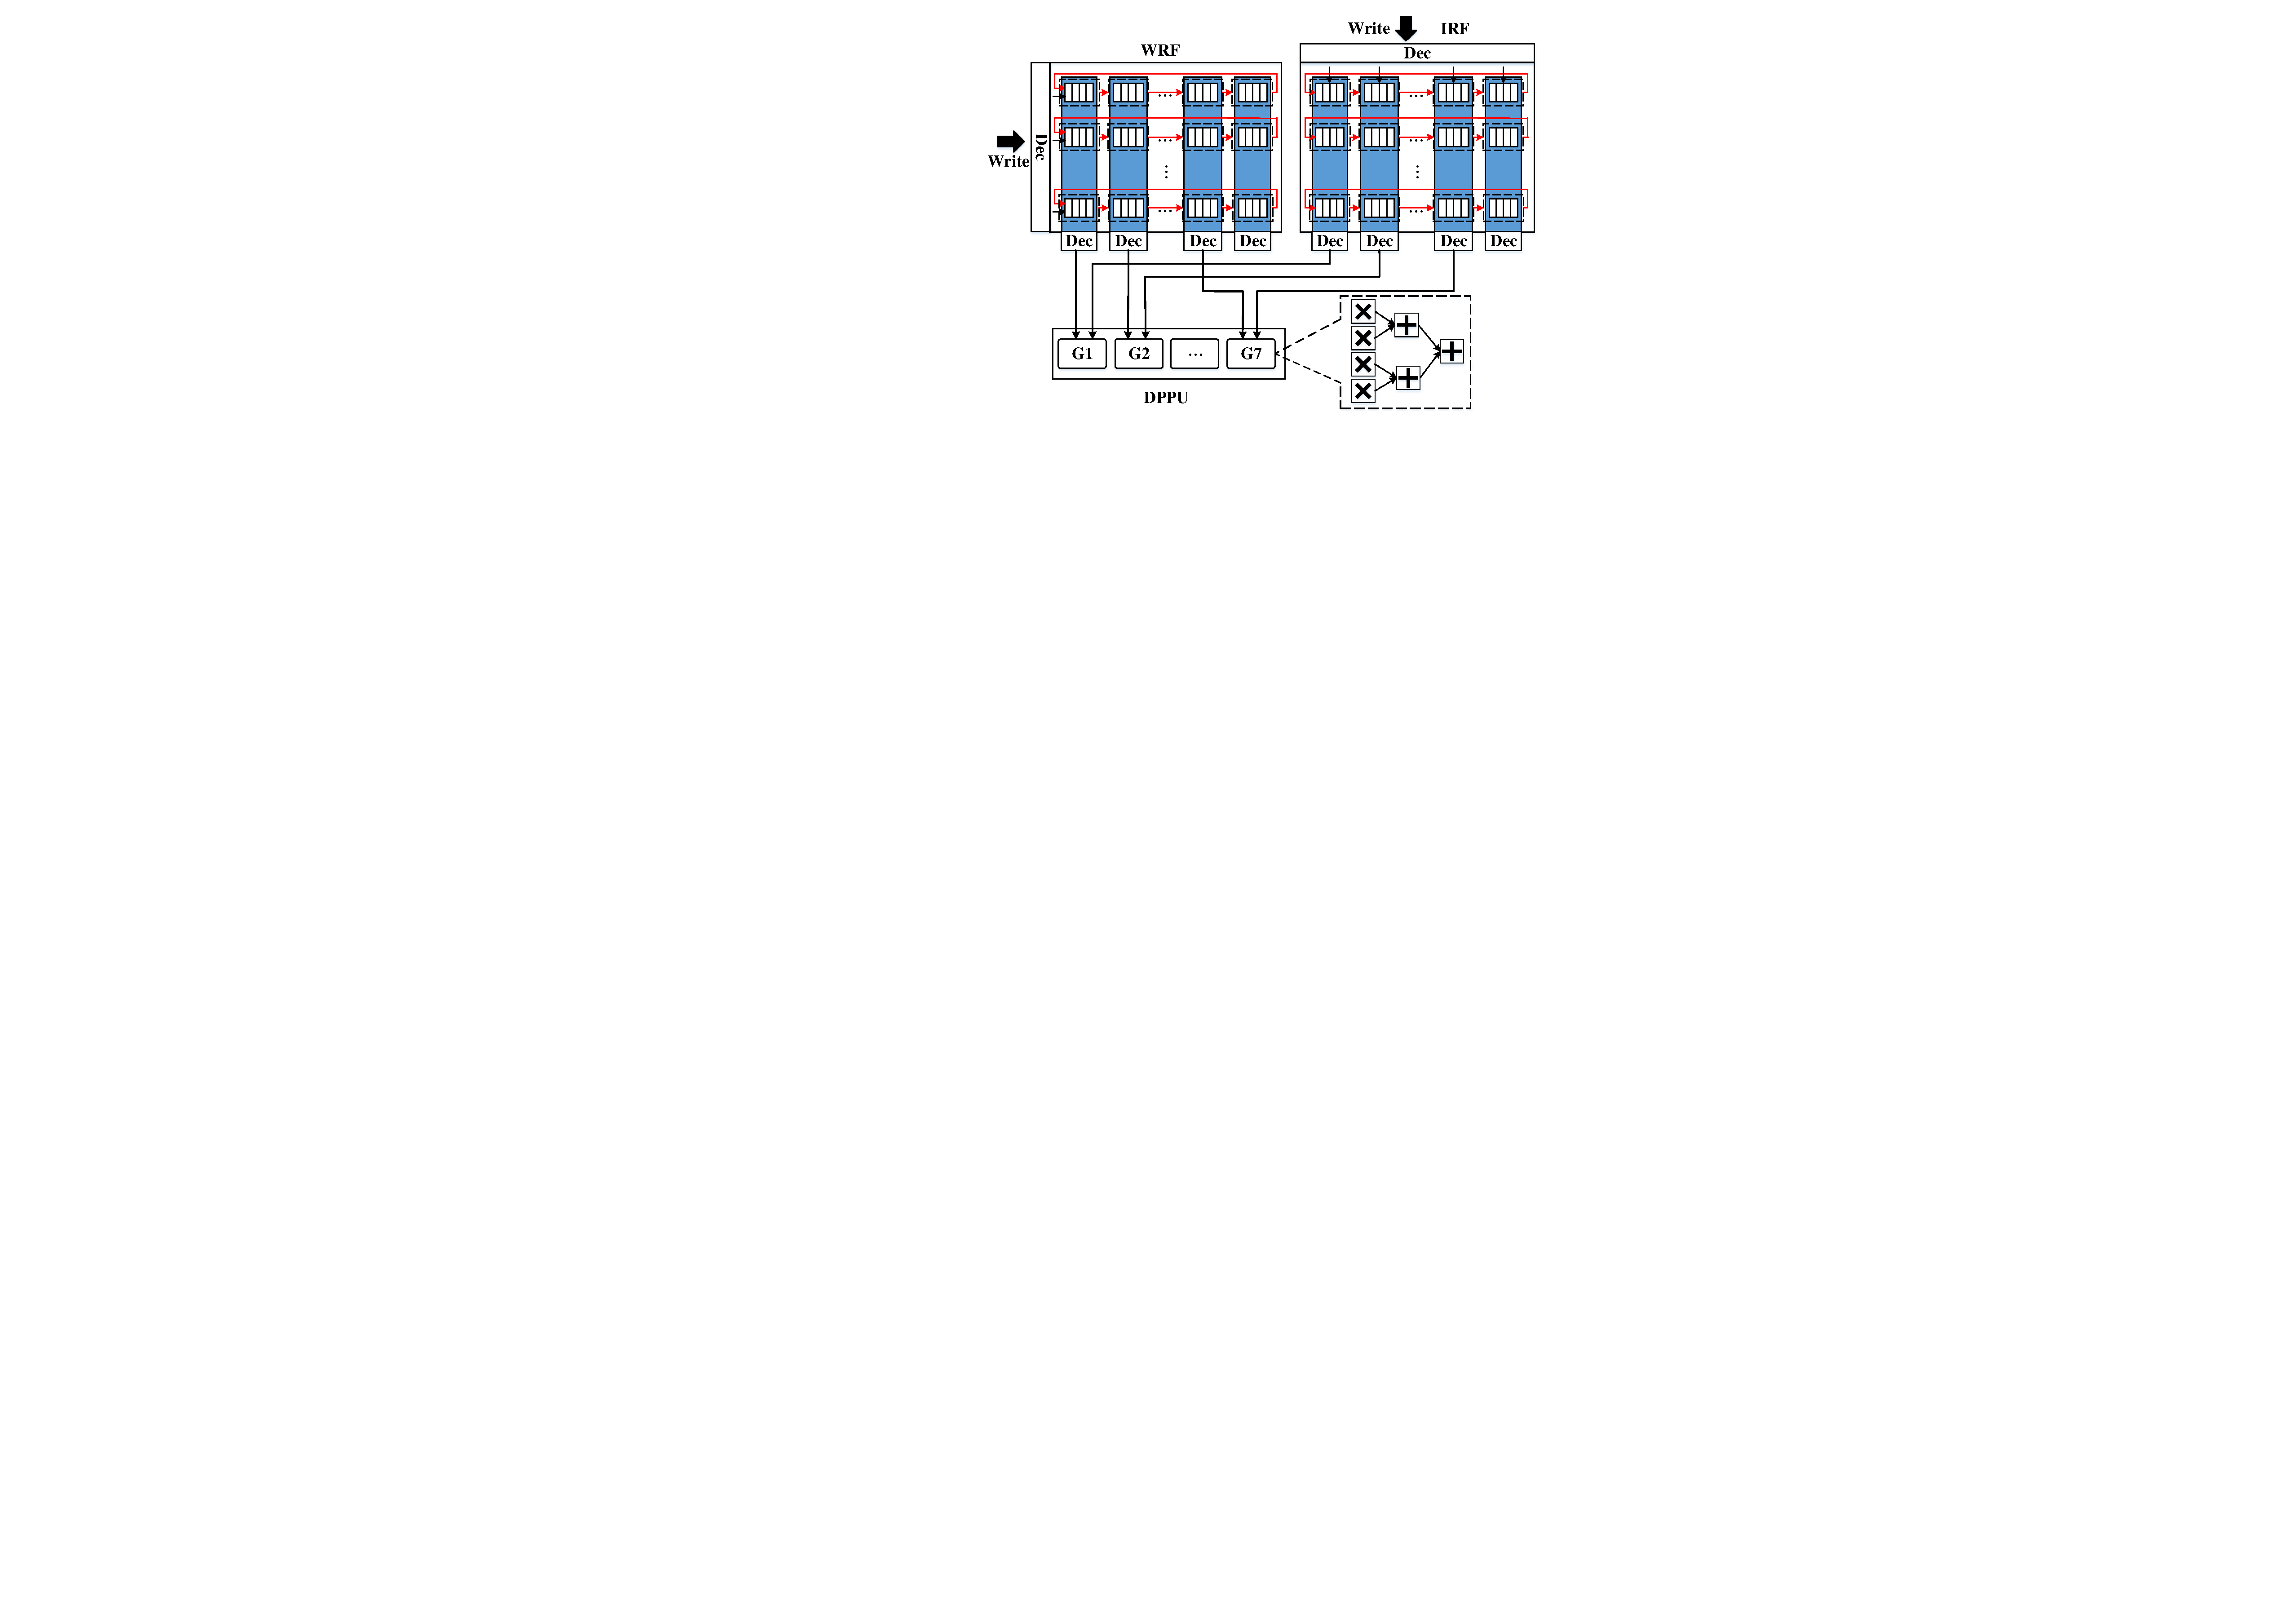
\includegraphics[width=0.7\linewidth]{images/HyCA-fig7.pdf}}
            \caption{Organization of the Weight Register File (WRF) and Input Register File (IRF). It shows how the register files are connected with a grouped DPPU with different number of computing groups.}
            \label{fig:reg}
            \vspace{-1em}
\end{figure}




\textbf{Register Files}

The IRF and the WRF are used to back up the data read from input buffer and weight buffer, and then supply the data to the DPPU for the recomputing. As the 2-D computing array and the DPPU have different dataflows for the neural network computing, the weight register file is written in column-wise manner but read in row-wise manner as shown in Figure \ref{fig:reg}. When the DPPU is split into multiple groups, these groups will be responsible for different faulty convolution operations and they need to read different rows of WRF and IRF at the same time. Although a straightforward multi-port register file can fulfill the concurrent register file read, it will induce substantial hardware overhead according to \cite{Energy2003Aneesh,A2012Chang}. 

While we observe that each computing group in DPPU has only a small number of PEs and they cannot consume a single row of inputs and weights in a single cycle. As a result, the straightforward multi-port register file actually has the bandwidth wasted. With this observation, we also have the register files split into groups in row direction such that each group of the register file can be read independently by the corresponding computing group in the DPPU. In this case, each register file has only a single read port, but each computing group can only read a segment of the data in the register files as indicated by the blue color. While an output feature recomputing on DPPU needs an entire row of data in the register files, we have each row of the registers organized as a circular shift register. With the shift register, different segments of the data in a row can be obtained by the corresponding computing group in DPPU in a few cycles. At the same time, the amount of data fed to each computing group can be fully utilized. Moreover, we notice the read port data width of the register files is not necessarily equal to the DPPU size. When the DPPU size is larger than the register file data width, more read ports can be added to some of the register file groups rather than the entire register file. When the DPPU size is smaller than the register file data width, some of the register file groups do not even need a read port as shown in Figure \ref{fig:reg}. Thereby, the DPPU size can be scaled conveniently and it will not be limited by the register file sizes. 

\subsubsection{Fault Detection with HyCA}
On top of the fault mitigation, DPPU can also be utilized to conduct fault detection at runtime. The basic idea is to have the DPPU to recompute the operations on a PE in the 2-D computing array. Then, we have the computing results compared to check if the PE in the 2-D computing array is faulty. By scanning all the PEs in the 2-D computing array sequentially, we can determine if the 2-D computing array is faulty. While the DPPU always starts the recomputing $Col$ cycles later, the computing result of a PE to be checked is already updated or written to the output buffer when the DPPU completes the recomputing. To address the problem, we have the computing results to be checked buffered in a checking list buffer (CLB) as shown in Figure \ref{fig:detection}. As the fault detection scanning is conducted sequentially, a simple on-chip buffer can fulfill the requirements. When the DPPU completes the recomputing, the fault detection module can have the results compared with that stored in the CLB.  

\begin{figure}[tb]
    \setlength{\abovecaptionskip}{-1pt}
    \setlength{\belowcaptionskip}{-10pt}
        \center{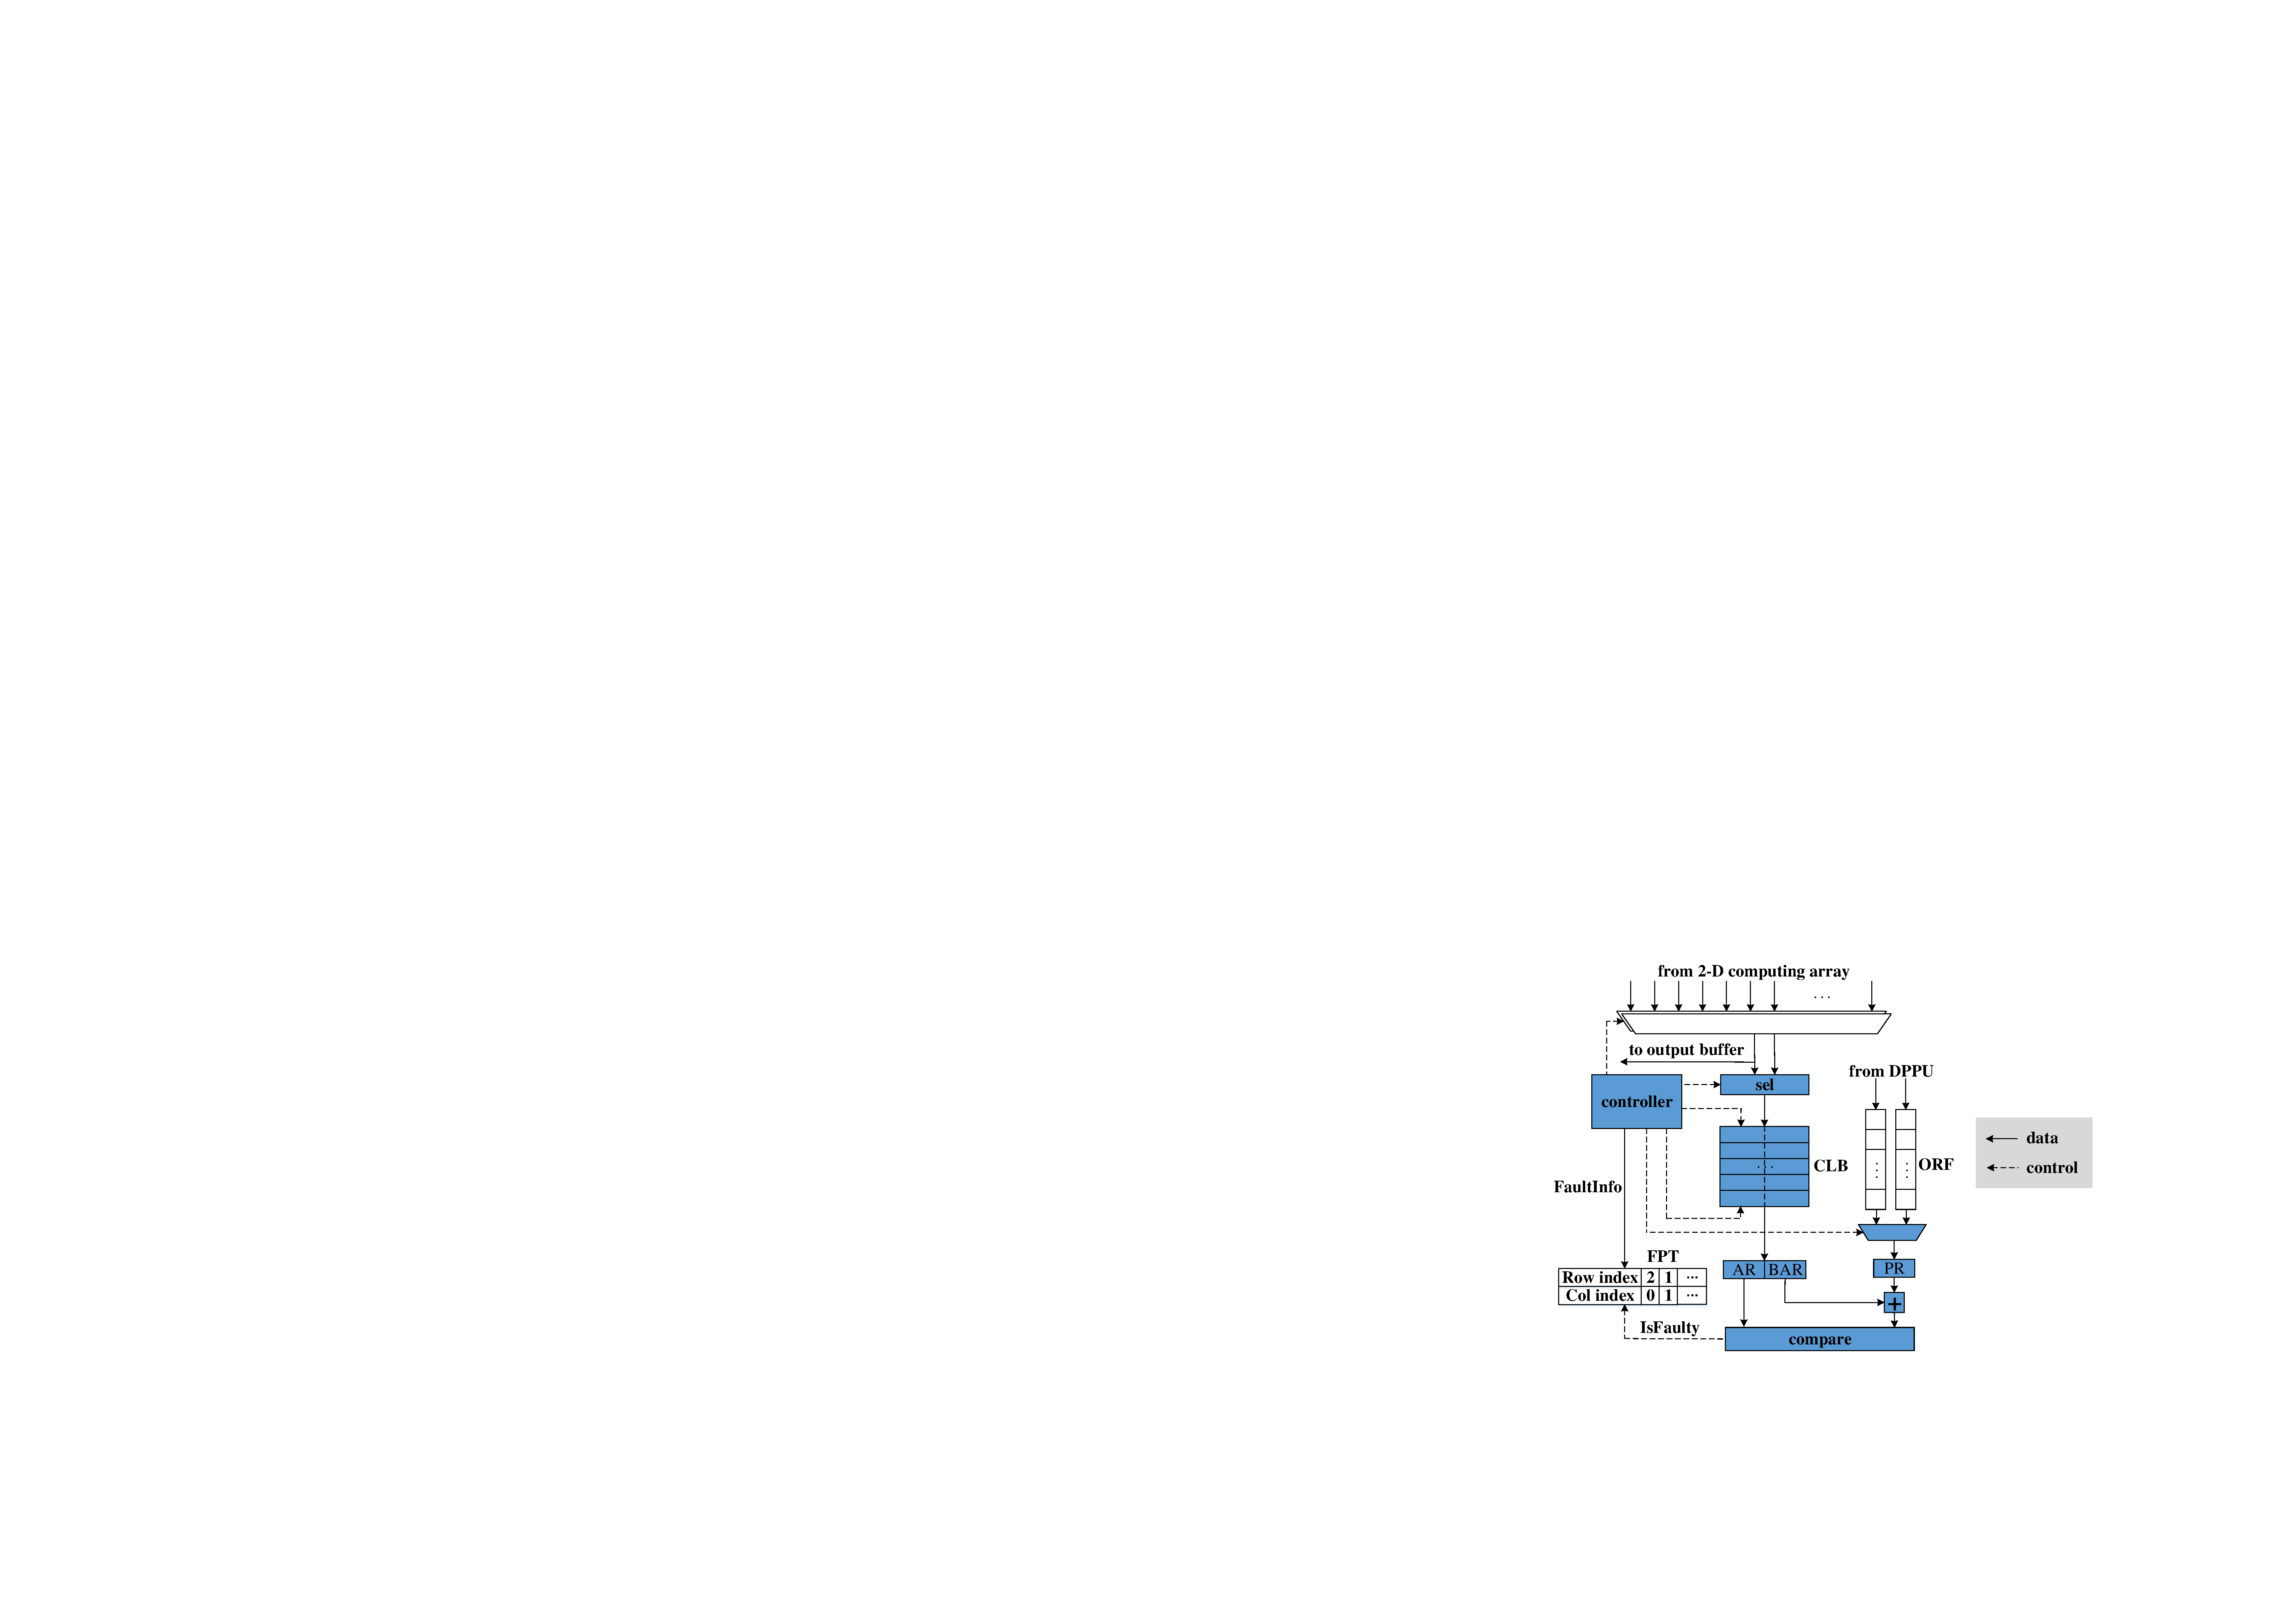
\includegraphics[width=0.7\linewidth]{images/HyCA-fig8.pdf}}
            \caption{Structure of the Fault-Detection Module.}
            \label{fig:detection}
            \vspace{-1.5em}
\end{figure}

As hard faults in a PE can usually lead to computing errors of most of the computation, we do not have to compare the final output feature computing results for the fault detection. Instead, we can compare the partial computing results of a PE for the fault detection such that the fault detection can be faster and more efficient. Since the DPPU conducts the processing in parallel, we have the partial computing result (PR) produced by a single DPPU group in a single cycle compared in this work. Different from the DPPU, PEs in the 2-D computing array have the computing results accumulated continuously before the entire output feature processing is completed. Suppose only one DPPU group is reserved for the runtime fault detection and the DPPU group includes $S$ PEs. To enable the comparison for the fault detection, we have both the base accumulated results (BAR) and the accumulated results (AR) calculated $S$ cycles later stored in the CLB. In the next cycle, another pair of the BAR and the AR from different PEs will be stored accordingly. As the weights and input features are stored in their register files for only $Col$ cycles, we only have $Col$ ARs and BARs stored in the CLB. While the CLB is also organized in Ping-Pong manner, the total size of the CLB is $4 \times W \times Col$ Bytes where $W$ denotes the width of the accumulator in PEs. 

According to the recomputing dataflow, the reserved DPPU group performs the recomputing $Col$ cycles later. Unlike the fault-tolerance oriented recomputing, the fault-detection oriented recomputing only conducts the dot-production of $S$ weights and input features rather than $Col$ weights and input features. The results of the DPPU will be compared with the corresponding results stored in the CLB for the fault detection. Basically, AR will be compared to the addition of PR and BAR. When a faulty PE is detected, the faulty information i.e. the fault PE row index and column index will be updated to the FPT. One comparison can be done per cycle, so it takes the fault detection module $Col$ cycles to complete the comparison with the stored results in CLB. Accordingly, it takes the fault detection module $Row \times Col + Col$ cycles to complete the fault detection of the whole 2-D computing array. When a DPPU group has more PEs included, it needs to check a partial result with more computation. As a result, the fault detection time is independent with the number of PEs in the DPPU group. While the fault detection time is already much smaller than the processing time of a normal neural network layer, it is fast enough to detect the computing errors. To avoid the frequent fault detection, the fault detection module can be activated periodically in a larger time range depending on the requirements of the applications. In addition, the fault detection module can reuse the majority of the fault recovery design, it induces only some simple controlling logic and a small CLB, and consumes negligible chip area.

\subsection{Experiment Result Analysis}
\subsubsection{Experiment Setup}
\textbf{Accelerator Configurations} The proposed deep learning accelerator with HyCA is implemented in Verilog and synthesized with Design Compiler under TSMC 40nm technology. The computing array size and DPPU size are set to be $32\times 32$ and 32 respectively. The input feature buffer size is 128KB, output feature buffer size is 128KB and the weight buffer size is 512KB. The computing of DPPU is delayed by $D=32$ cycles after the 2-D computing array, so both the weight register file size and the input register file size are set to be $2 \times 32 \times D = 2048$ i.e. 2KB. The output register file in DPPU is 64-byte. The fault PE table size is $32 \times 10$bits. Each entry of the table includes 5-bit row index and 5-bit column index of a faulty PE. Both the data width of weights and input feature data is 8-bit. To ensure the resilience of the DPPU, we have every four multipliers in the DPPU grouped and equipped with a redundant multiplier, and every three adders in the DPPU grouped and protected with a redundant adder. For the 2-D computing array, we have three classical redundancy approaches including RR, CR, and DR implemented and each redundancy implementation is equipped with 32 redundant PEs.

\textbf{Fault Models} To evaluate the reliability of the redundancy designs comprehensively, we have two different fault distribution models including the random distribution model and the clustered distribution model implemented. For the random distribution model, the faults are randomly distributed across the entire computing array. For the clustered distribution model which is usually used to characterize the manufacture defects, the faults are more likely to be close to each other and the model proposed in \cite{meyer1989modeling} is applied in this work. Meanwhile, we notice that the influence of hardware faults is related with the fault distribution, so we generate 10000 configurations randomly for each fault injection rate and average the evaluation in the experiments. 

As hard errors are mainly caused by the manufacturing defects, aging, and wear-out, which can be affected by many complex factors such as application requirements, working status, and the fabrication, there is still a lack of references investigating the practical PER setup and prior fault-tolerant designs typically have distinct error rate setups \cite{liu2011resilient, li2008understanding, abdullah2020salvagednn, analyzing2018vts}. In this case, we evaluate the hard error rate in a large range and seek to demonstrate when we can ensure reliable computing. Then, we expect the users to choose the target hard error rate for their specific fault-tolerant designs. In addition, since we mainly focus on the reliability of the regular 2-D computing array in a deep learning accelerator, we use PE error rate (PER) as the fault injection metric similar to the works in \cite{zhang2018analyzing} and \cite{qian2016optimal}. Meanwhile, we notice that bit error rate (BER) that refers to the number of bit errors over the total number of memory bits is directly related with definition of the hard error on chips, and it has been widely utilized as a metric for fault analysis in many prior works \cite{mittal2020survey}\cite{neggaz2018reliability}\cite{ares2018dac}. Thus, we convert the BER to PER with (Equation \ref{eq:error_rate}) mentioned in Section \ref{sec:motivation} assuming that any bit error in a PE will cause the PE failure. While BER typically ranges from $1 \times 10^{-7}$ to $1 \times 10^{-3}$, PER ranges from 0$\%$ to 6$\%$ according to the conversion.  


\textbf{Neural Network Benchmark} To evaluate the performance of a typical DLA with the proposed fault-tolerant HyCA, we have a set of representative neural network models including Alexnet, VGG, Resnet, and YOLO used as the benchmark. Alexnet, VGG and Resnet are classical models used for image classification, while YOLO is mostly used for object detection. All the models are pre-trained on ImageNet. We measured the performance of the benchmark on the DLAs with different redundancy design approaches using Scale-sim\cite{samajdar2018scale}. Since Scale-sim is relatively slow, it is difficult to obtain the performance of all the random fault configurations directly. In this experiment, we determined the final valid computing array setups of all the fault configurations and performed the simulation on only the unique computing array setups. As many fault configurations lead to the same computing array setups eventually, this approach greatly reduces the simulation time. Finally, we averaged the resulting performance based on the generated fault configurations.

\begin{figure}
\setlength{\abovecaptionskip}{-2pt}
\setlength{\belowcaptionskip}{0pt}
	\center{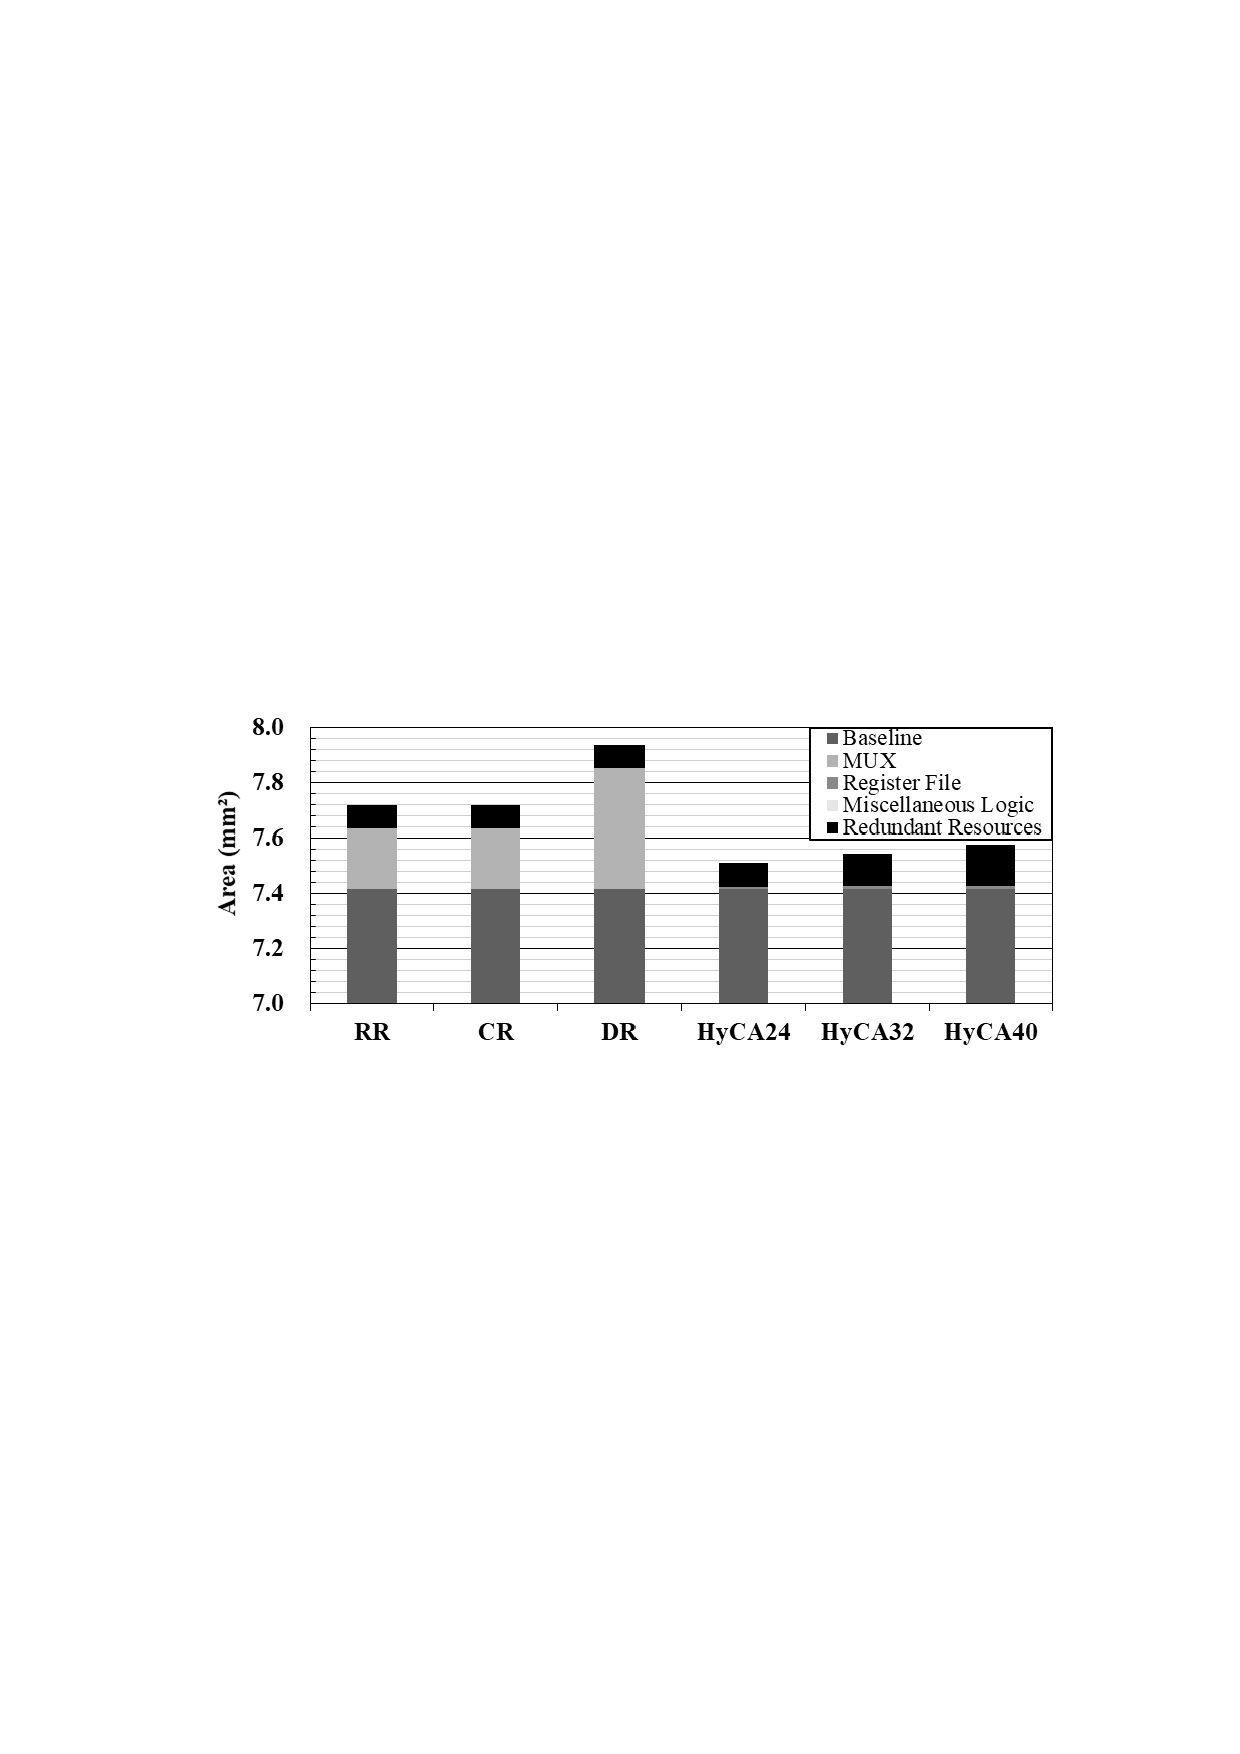
\includegraphics[width=0.9\linewidth]{images/HyCA-fig9.pdf}}
    \caption{Chip area under different redundancy approaches.}
\label{Circuit area}
\vspace{-1em}
\end{figure}

\subsubsection{Chip Area Overhead Comparison} \label{sec:chip-area}
Figure \ref{Circuit area} illustrates the chip area of the DLAs with different redundancy approaches including RR, CR, DR, and HyCA. Particularly, we have three HyCA-based designs with different DPPU sizes compared. The DPPU size of HyCA24, HyCA32, and HyCA40 is 24, 32 and 40 respectively. According to the comparison Figure \ref{Circuit area}, the HyCA-based designs exhibit much less redundancy overhead compared to the classical redundancy designs. The redundancy overhead of the HyCA-based designs mainly consist of the redundant PEs and the register files, while the redundancy overhead of the RR-based, CR-based, and DR-based designs are mainly attributed to the MUX and the redundancy PEs. As the 2-D computing array size is $32 \times 32$, the number of redundant PEs in RR-based, CR-based, and DR-based designs is the same and the chip area caused by the redundant PEs is also equal. While HyCA has different PE structures, i.e. independent multipliers and adders rather than MACs, and additional redundant PEs, the chip area of the redundant PEs is larger given the same DPPU sizes. In contrast to the chip area of the redundant PEs in HyCA, the added small Ping-Pong register files in HyCA consumes much less chip area. Different from HyCA, RR, CR and DR include a large number of MUX to enable the replacement of faulty PEs with the redundant PEs. These MUX take up substantial chip area and dominate the redundancy overhead. 

\subsubsection{Reliability Comparison}
To evaluate the reliability of the DLAs, we propose two metrics that can be applied for different applications. One of them is the fully functional probability and it shows the probability that the DLA can be fully functional without any performance penalty. It is preferred by the mission-critical applications that do not allow any performance degradation nor model modification because any system modification may require expensive and lengthy safety evaluation and certification. The experiment is shown in Figure \ref{fig:survival}. It shows that HyCA outperforms the three classical redundancy approaches and the advantage gets enlarged under the clustered fault distribution. The main reason is that each redundant PE in RR, CR and DR can only be utilized to replace a single faulty PE in a row, a column, and a row-column pair respectively. When multiple faults occur in the same protected region, these redundancy approaches fail to recover the faulty 2-D computing array and the design will not be fully functional. Unlike these classical redundancy approaches, HyCA allows arbitrary faulty distribution and can perfectly repair the computing array as long as the number of faulty PEs in the 2-D computing array does not exceed the DPPU size. Thereby, the fully function probability of HyCA is not sensitive to the fault distribution models. As DPPU size is set to be 32 and the 2-D computing array size is $32 \times 32$ in this example, the fully functional probability drops to 0 immediately when the number of fault PEs exceeds 32 at 3.13\% PER. As the PEs in the DPPU can also be faulty, the fully functional probability of HyCA starts to drop when the number of faulty PE is close to 32 and the PER is slightly lower than 3.13\%.

\begin{figure}
\setlength{\abovecaptionskip}{-10pt}
\setlength{\belowcaptionskip}{-2pt}
	\center{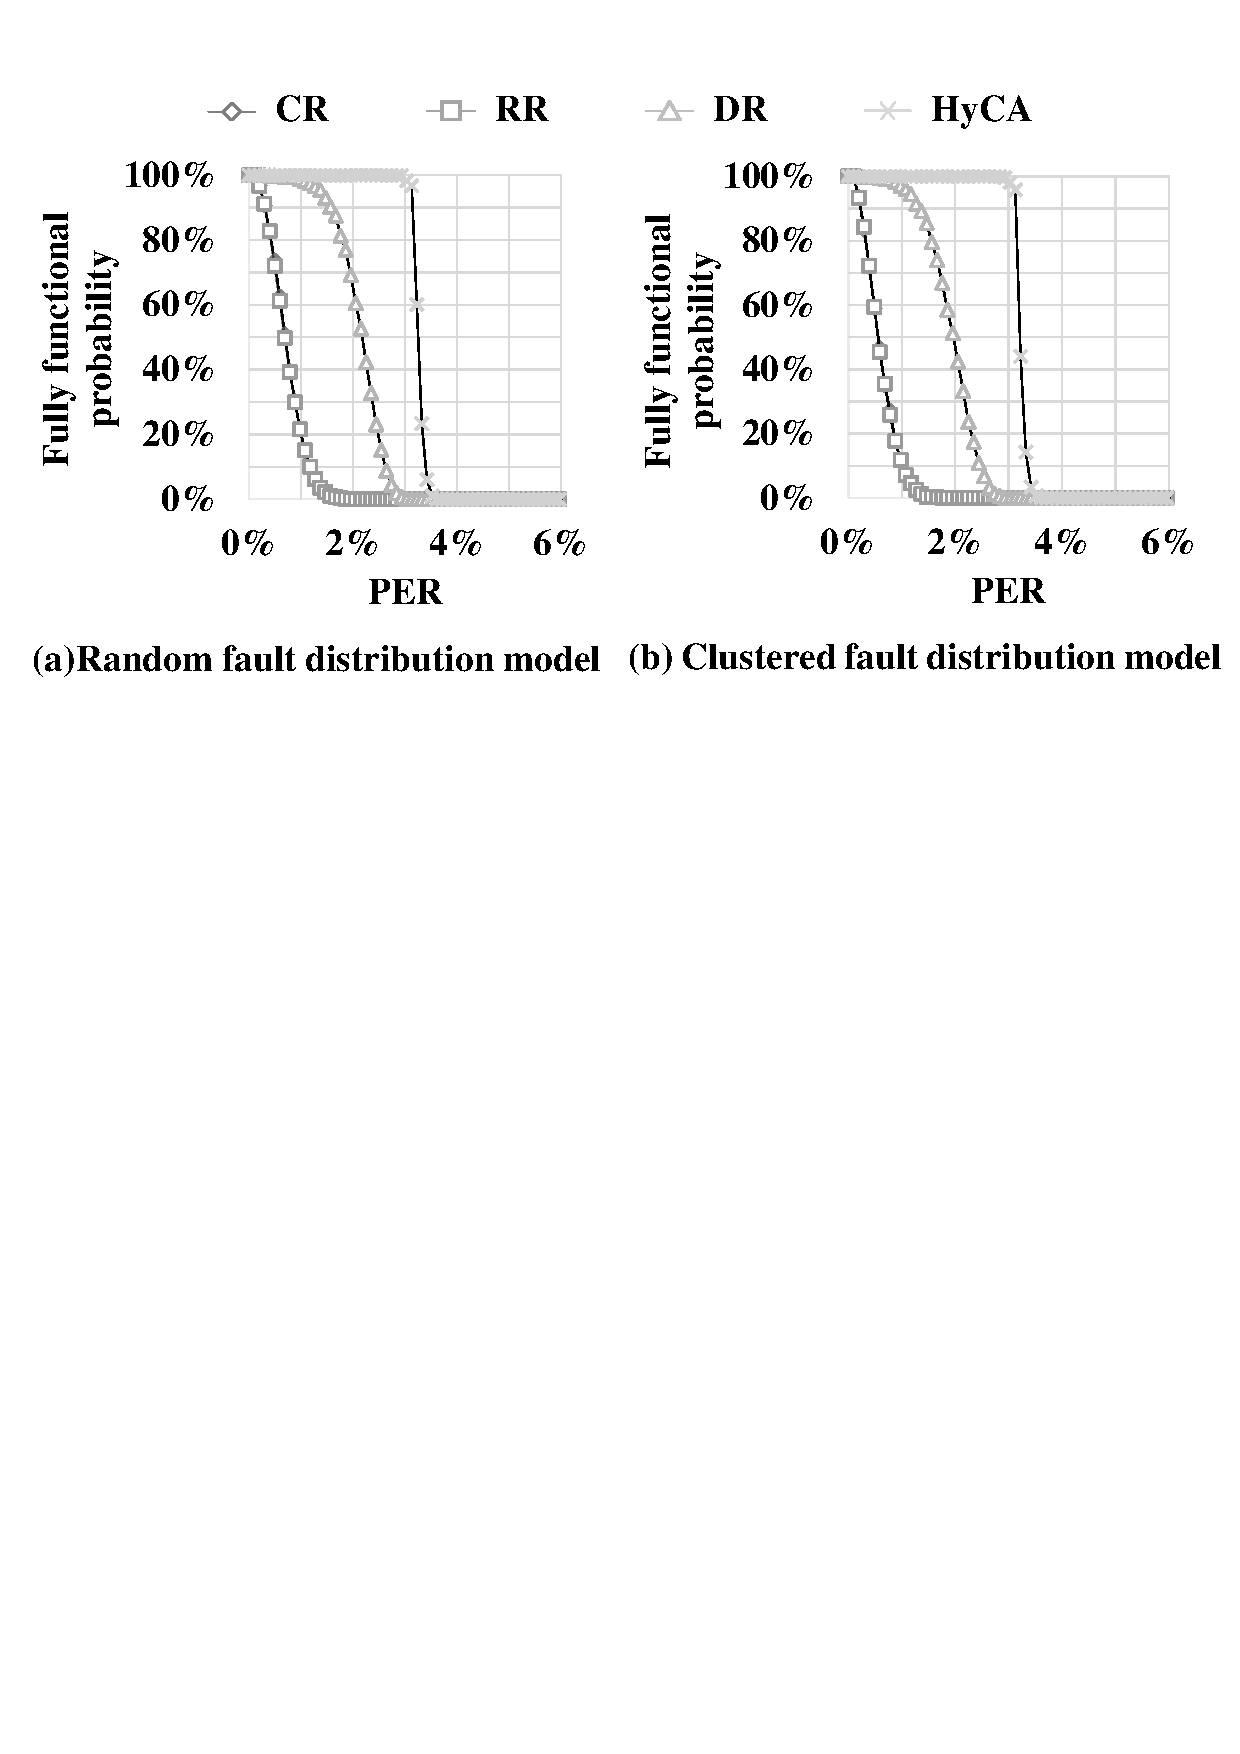
\includegraphics[width=1\linewidth]{images/HyCA-fig10.pdf}}
    \caption{Fully functional probability of DLAs with different redundancy approaches.}
\label{fig:survival}
\vspace{-1.5em}
\end{figure}

The other metric is the normalized remaining computing power and it refers to the percentage of the remaining computing array size over the original 2-D computing array size. This metric is particularly important for the non-critical applications that do not require fully functional accelerators and allow the accelerators to be degraded, because the remaining computing array size determines the theoretical computing power and affects the performance of the deployed neural network models directly. In this work, we apply the acceleration degradation strategy mentioned in the end of Section \ref{sec:dataflow} and discard the faulty PEs in the granularity of a column when the redundant PEs are insufficient to mitigate all the faulty PEs. Although more aggressive degradation approaches are possible to achieve larger computing power, this approach is applied for more efficient model compilation, hardware implementation and memory accesses. 

\begin{figure}
\setlength{\abovecaptionskip}{-10pt}
\setlength{\belowcaptionskip}{-2pt}
	\center{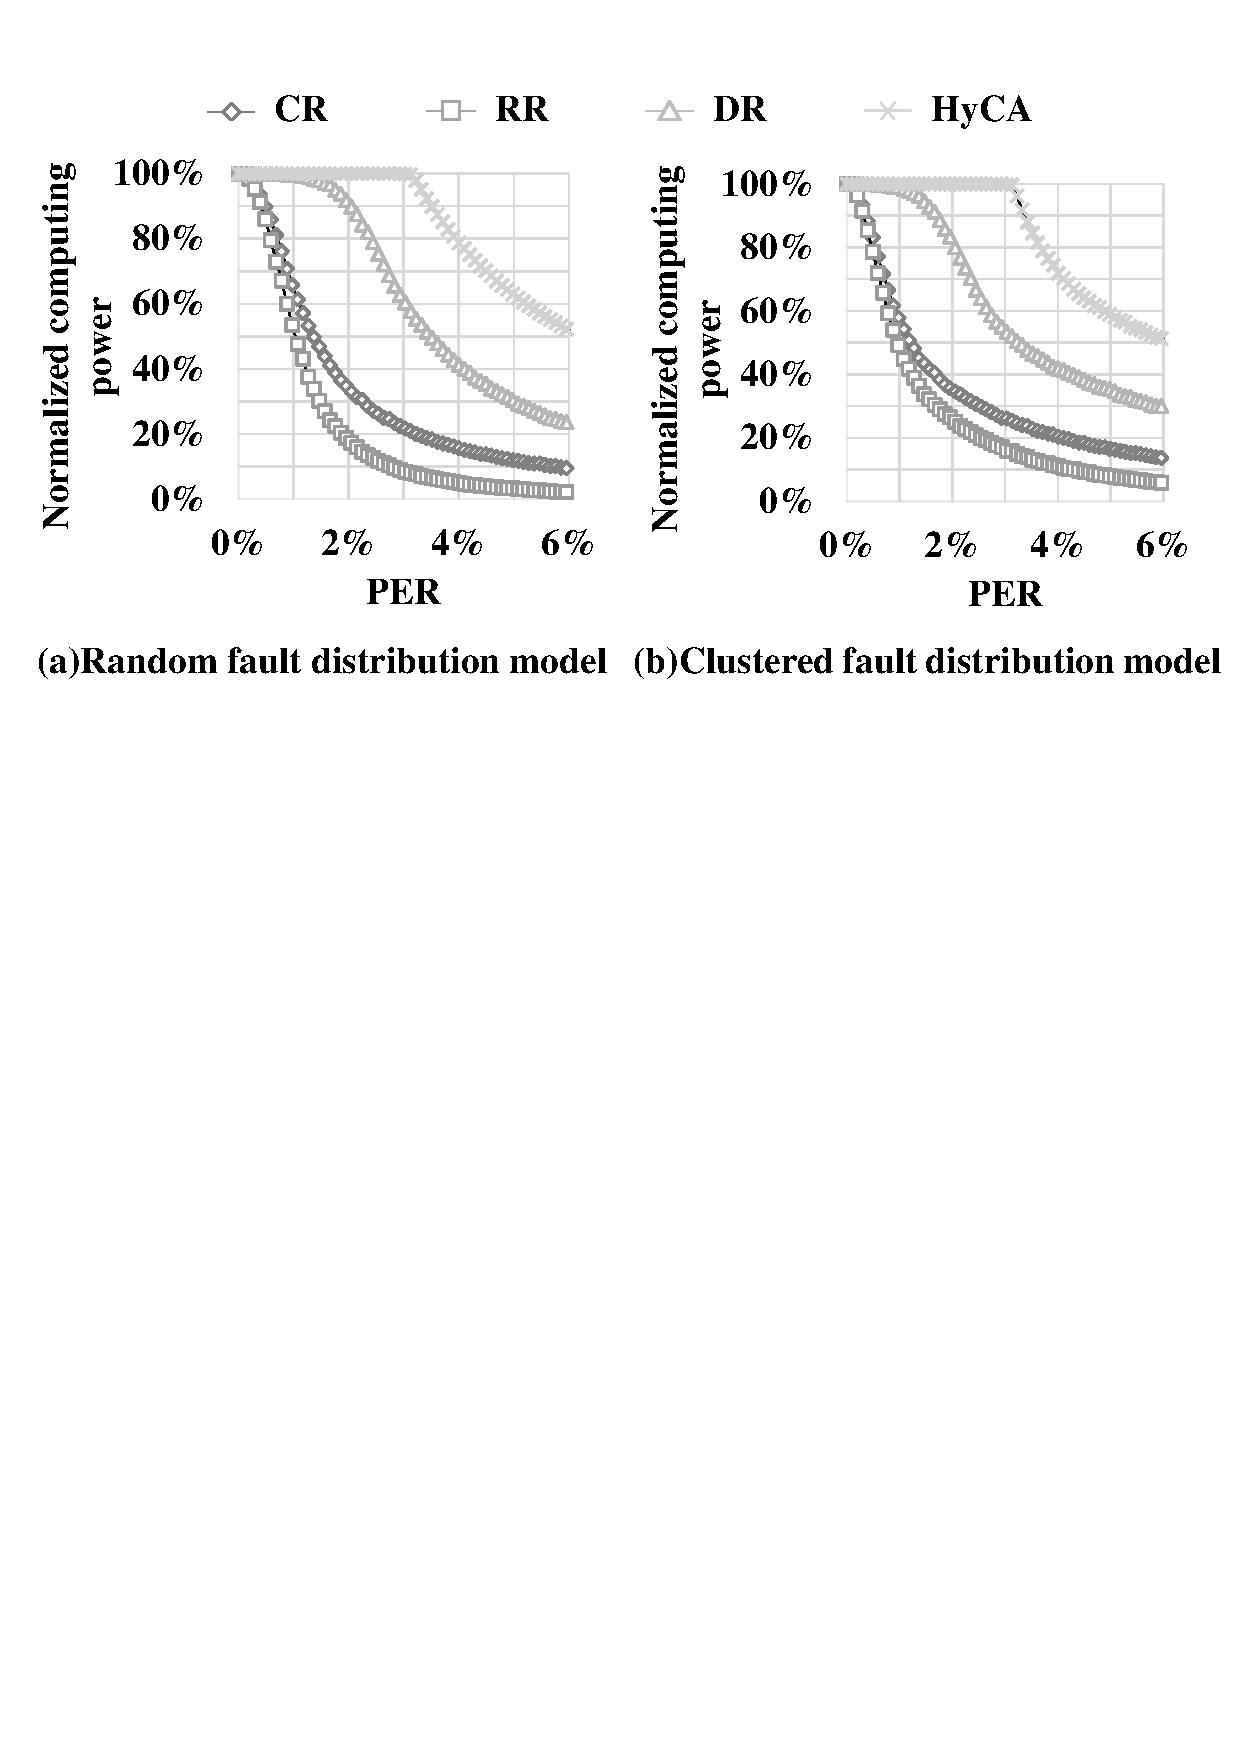
\includegraphics[width=0.99\linewidth]{images/HyCA-fig11.pdf}}
    \caption{Normalized computing power of DLAs with different redundancy approaches.}
\label{fig:available}
\vspace{-1em}
\end{figure}

Figure \ref{fig:available} reveals the computing power comparison of the different redundancy approaches. It can be observed that HyCA shows significantly higher computing power under all the different PER setups and the advantage also enlarges with the increase of the PER. This is mainly brought by the fault recovery flexibility of the HyCA that allows the DPPU to select the most critical faulty PEs to repair when the redundant faulty PEs are insufficient. Note that the most critical faulty PEs refer to the ones that can maximize the remaining 2-D computing array. By optimizing the faulty PE mitigation order, the remaining computing array can be larger. In contrast, each redundant PE can only repair a limited subset of the faulty PEs for the RR, CR and DR. There is little space left to optimize the faulty PE mitigation order. Thereby, the remaining computing power of RR, CR, and DR is much lower. As we choose to discard the faulty PEs that are failed to be repaired in the granularity of a column, RR cannot effectively shift the faulty PEs to a different column and has to discard the column whenever there are more than one faulty PEs. As a result, RR shows the lowest computing power even when the number of redundant PEs is the same with the other redundancy approaches.


\begin{figure}
\setlength{\abovecaptionskip}{-10pt}
\setlength{\belowcaptionskip}{-20pt}
	\center{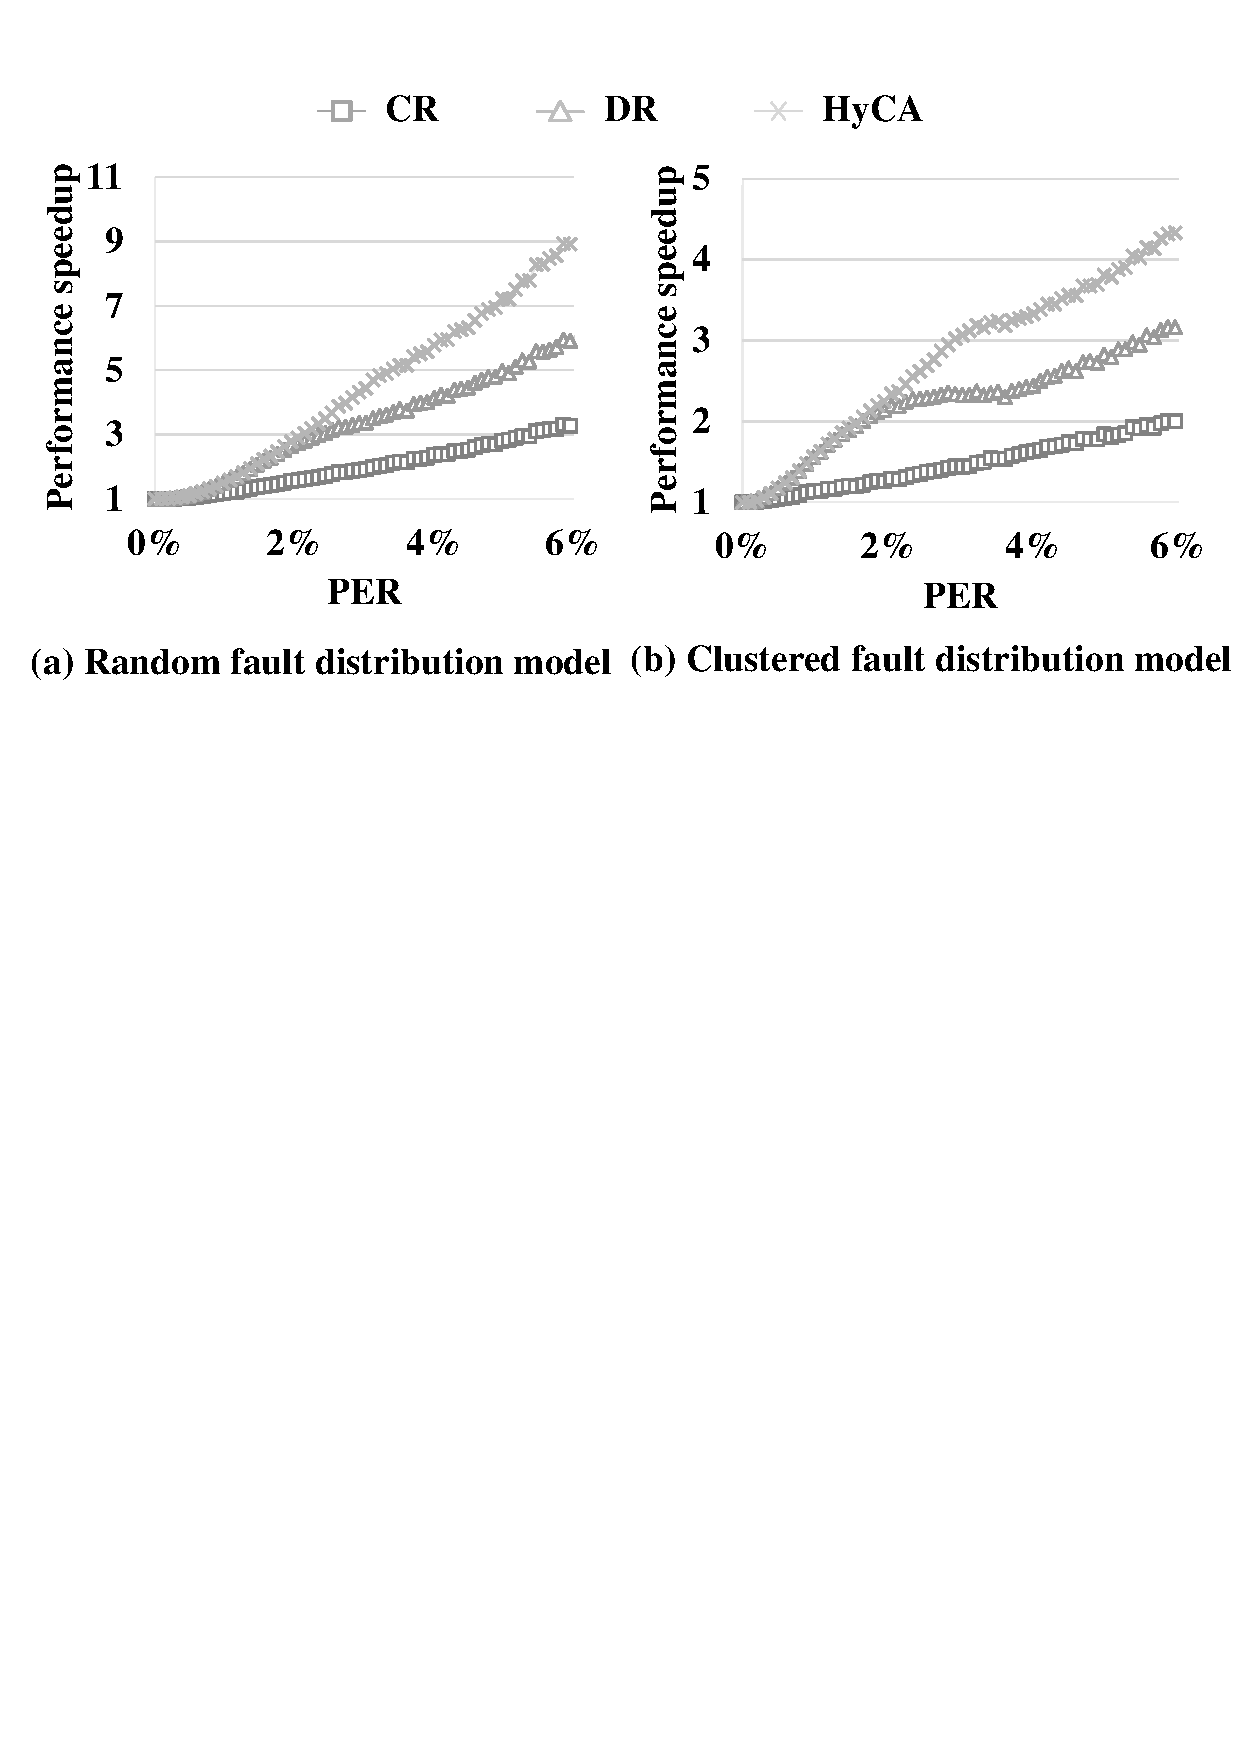
\includegraphics[width=1\linewidth]{images/HyCA-fig12.pdf}}
    \caption{Normalized performance of DLAs with different redundancy approaches}
\label{fig:ratio}
\vspace{-1em}
\end{figure}

\begin{figure}
\setlength{\abovecaptionskip}{-2pt}
\setlength{\belowcaptionskip}{-10pt}
	\center{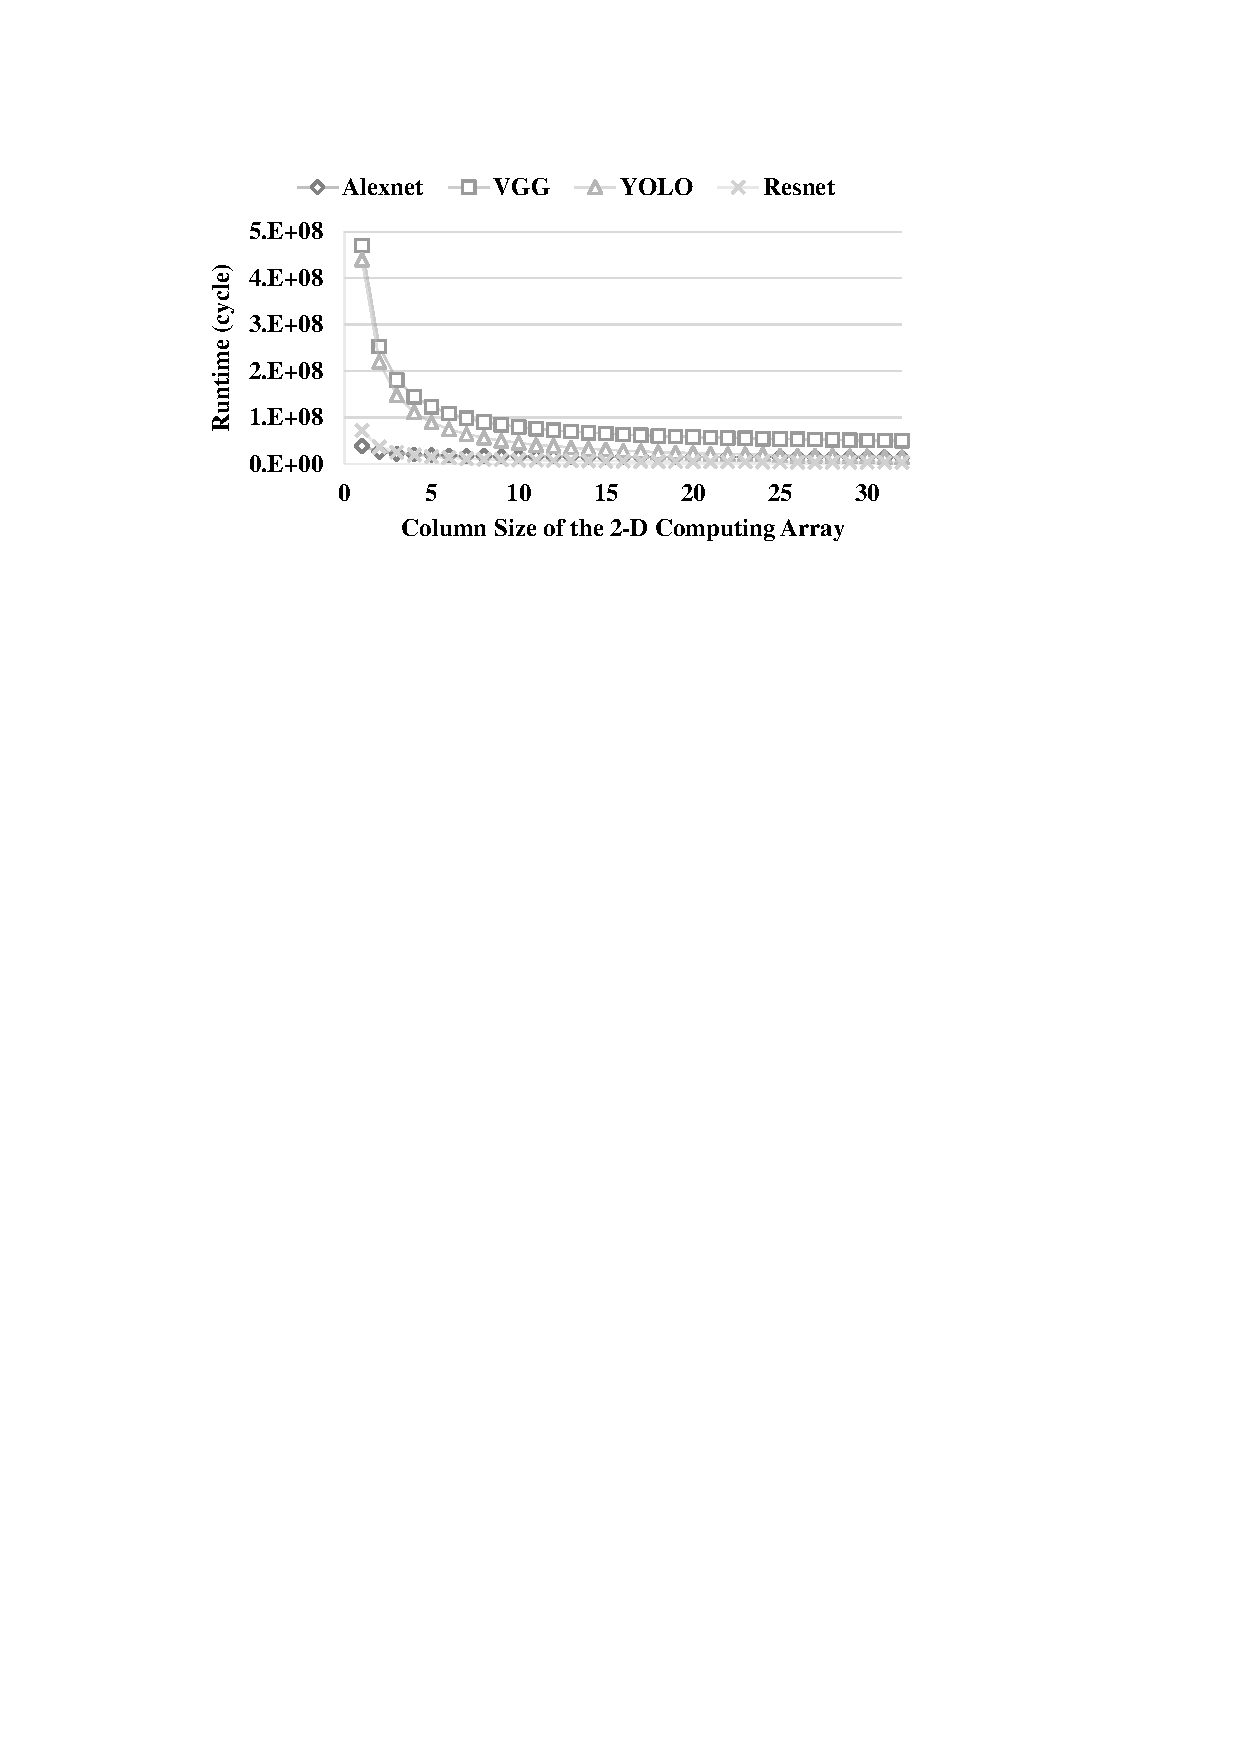
\includegraphics[width=0.8\linewidth]{images/HyCA-fig13.pdf}}
    \caption{Neural network runtime of the DLAs with different computing array sizes. Note that the row size of the computing arrays is fixed to be 32.}
\label{fig:model-performance}
\vspace{-1em}
\end{figure}

\begin{figure*}
\setlength{\abovecaptionskip}{-10pt}
\setlength{\belowcaptionskip}{0pt}
	\center{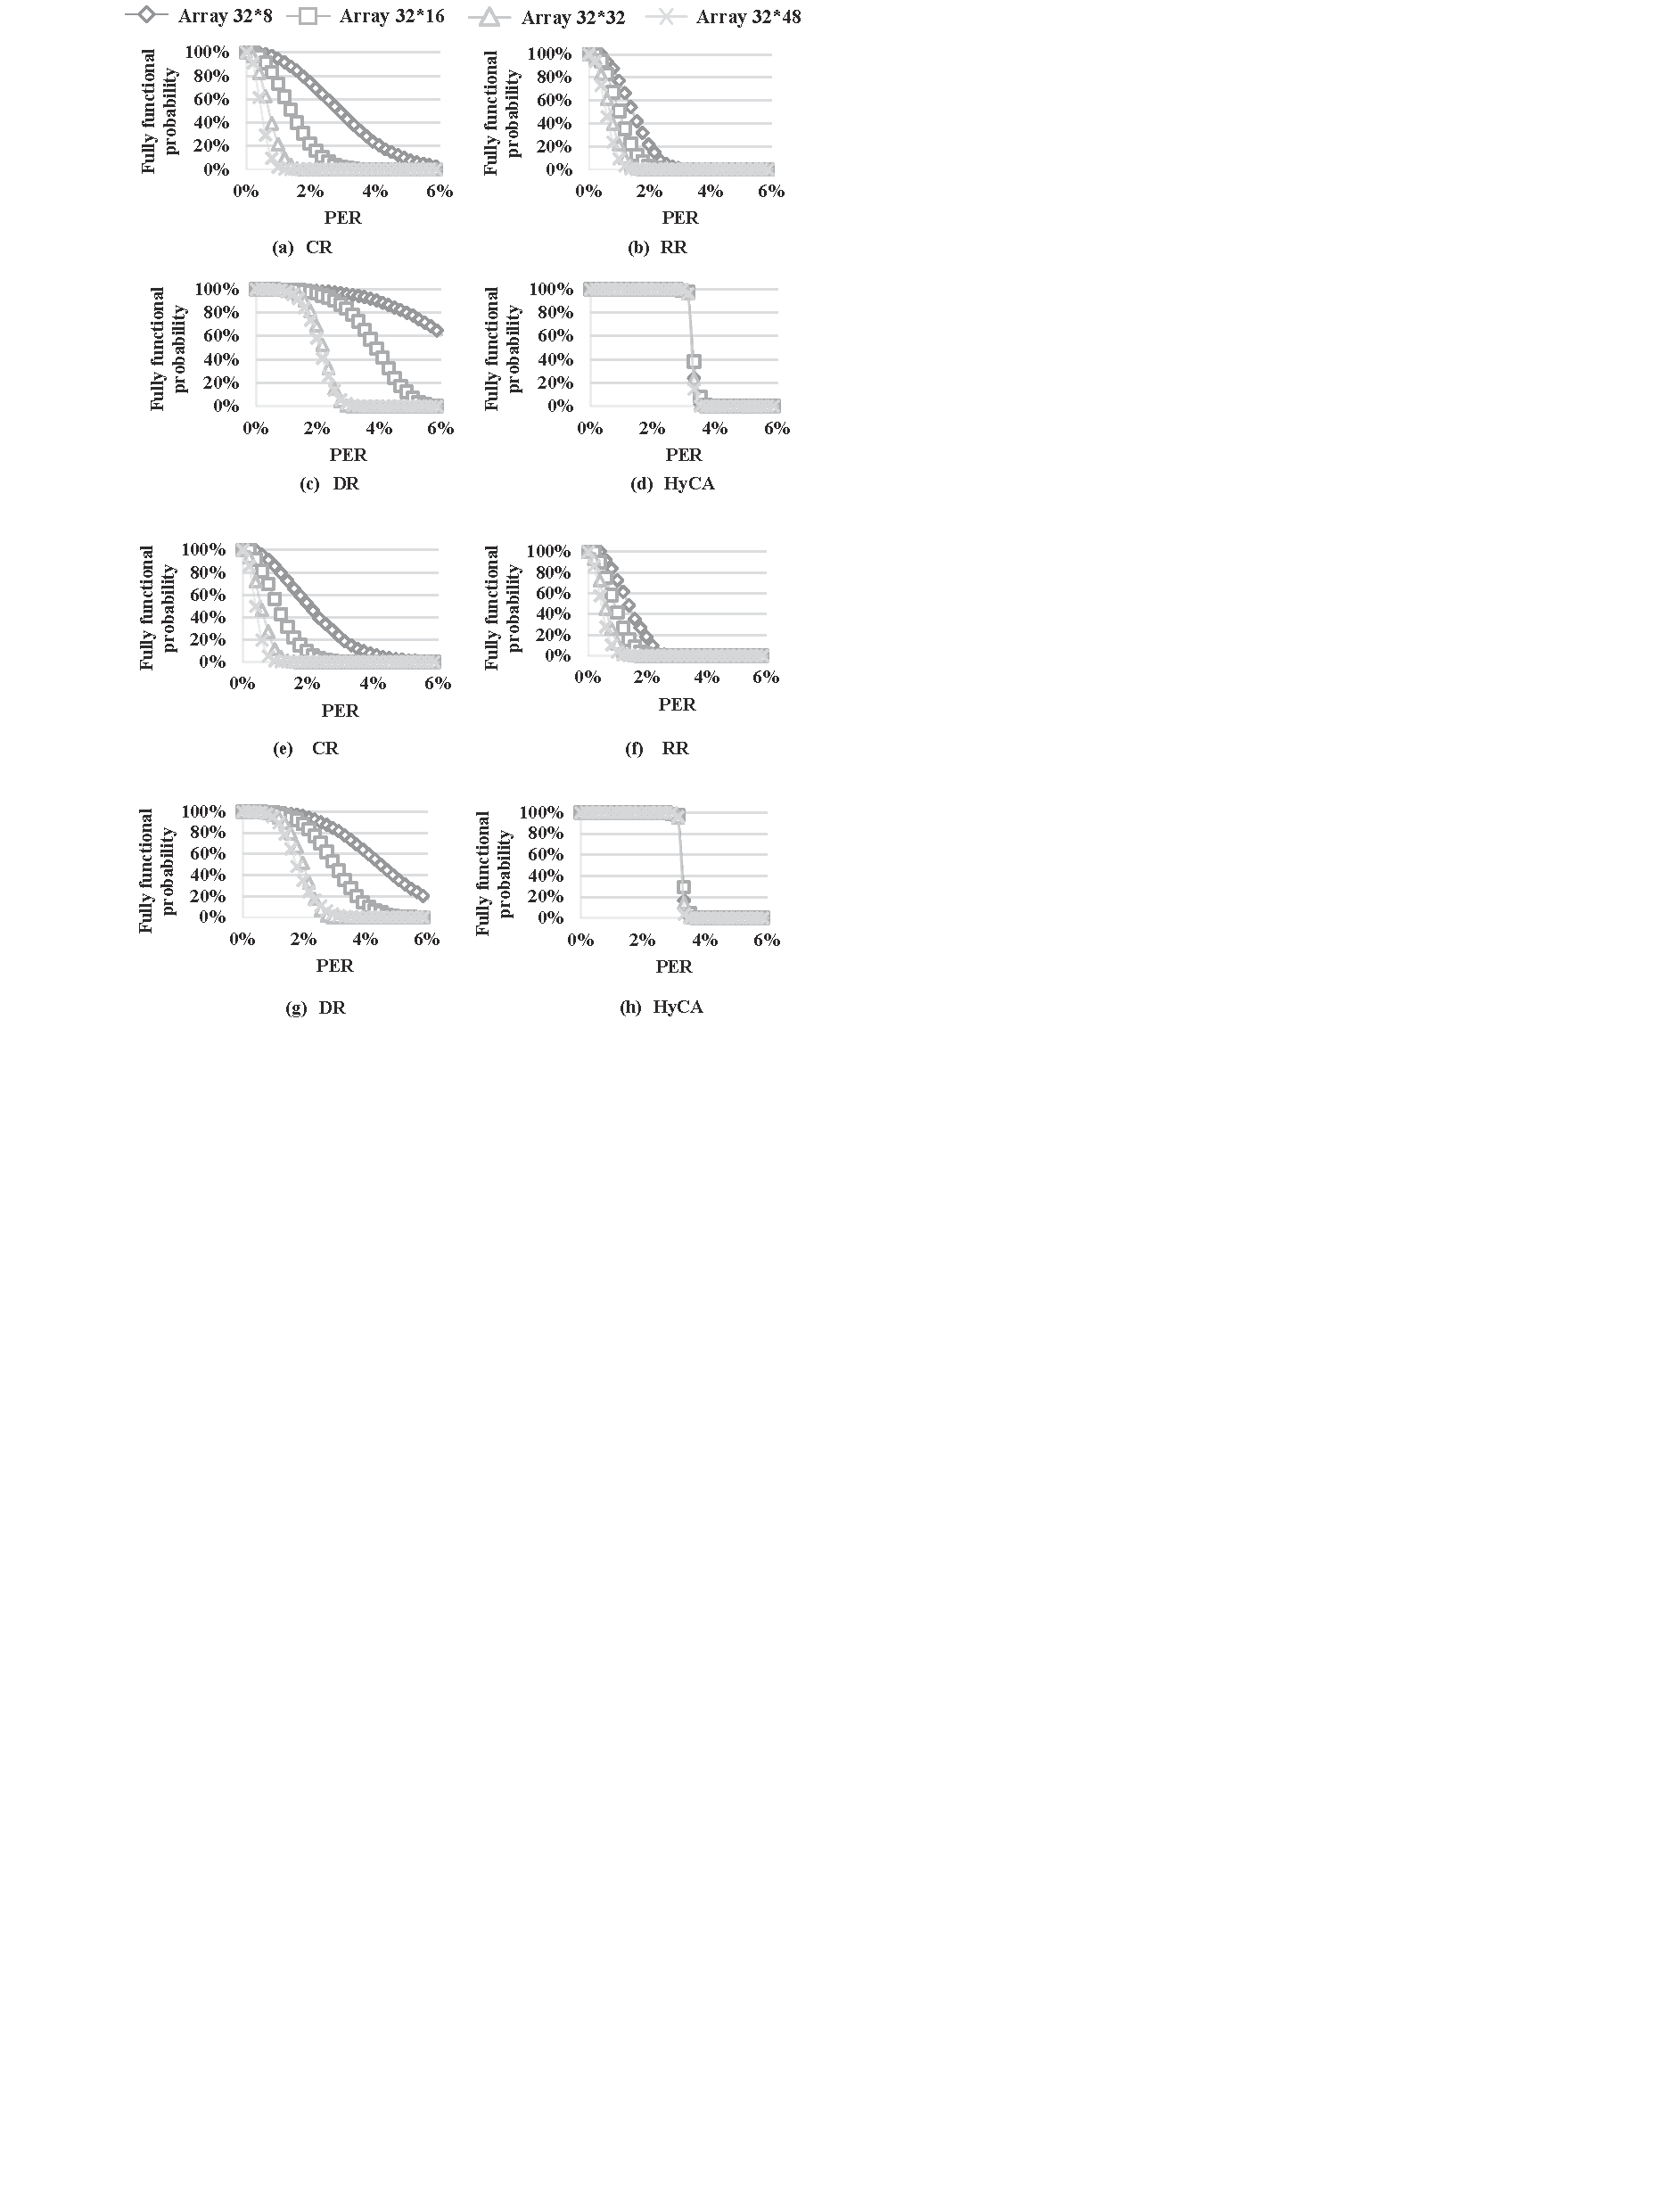
\includegraphics[width=1\linewidth]{images/HyCA-fig14.pdf}}
    \caption{Fully functional probability of the DLAs with different computing array sizes when they are protected with RR, CR, DR and HyCA respectively. Figure(a-d) are evaluated under the random fault distribution while Figure (e-h) are evaluated under the clustered fault distribution.}
\label{fig:scalability}
\vspace{-1em}
\end{figure*}

\subsubsection{Performance Comparison}
In order to evaluate the performance of the DLAs protected with the different redundancy approaches, we have the neural network benchmark deployed on the DLAs with Scale-Sim. The performance is normalized to that of the DLA protected with RR and the experiment result is shown in Figure \ref{fig:ratio}. It can be found that HyCA achieves much higher performance than the other redundancy approaches especially under relatively higher PER, which is roughly consistent with the experiment in Figure \ref{fig:available} though the neural networks also affect the performance. Particularly, the performance speedup goes up to 9X when the PER is around 6\% under the random fault distribution. The underlying reason for the higher performance speedup at higher PER is that higher PER indicates more faulty PEs in the 2-D computing array and leaves larger optimization space for the HyCA. 

Another observation is that the performance gap between HyCA and the other redundancy approaches is much smaller than the computing power gap. For instance, the computing power of HyCA is around 25X higher than RR when PER is 6\% under the random fault injection while the performance speedup is only 9X. This is mainly attributed to the fact that the neural network runtime varies dramatically under different computing array sizes as shown in Figure \ref{fig:model-performance}. When the remaining computing array size is large at lower PER, the runtime decreases much slower with the increase of the computing array size. In addition, some of the neural networks like VGG include some full connection layers that fail to make best use of the computing array. In fact, only a single column of PEs is used for the full connection operations given the output stationary dataflow and the larger remaining computing array in HyCA is underutilized, which also undermines the performance speedup.

\subsubsection{Redundancy Design Scalability Analysis}
As different applications may have distinct requirements of reliability and may also work under different fault environments, a scalable redundancy design can greatly alleviate the reliability design problems. In this subsection, we will investigate and compare the scalability of the different redundancy approaches under different computing array sizes. As the fully functional probability and the computing power is roughly positively related, we only use the fully function probability as the metric for the scalability evaluation to save the space. The number of redundant PEs in RR and CR is consistent with the corresponding computing array row size and column size respectively. Although the number of redundant PEs in DR is also equal to the diagonal size of the computing array, it cannot be directly applied to a non-square computing array. In this experiment, we divide the non-square computing array into multiple square computing arrays and apply the diagonal redundancy approach to each sub computing array independently. The number of redundant PEs in HyCA is set to be $Col$ to ensure a fair comparison where $Col$ refers to the column size of the computing arrays. 

The experiment result is shown in Figure \ref{fig:scalability}. It can be observed that the fully functional probability of RR, CR and DR under different PER setups vary dramatically when the computing array size changes. CR and DR have the same amount of redundant PEs on the different 2-D computing array sizes. Basically, the redundancy intensity, i.e. the average redundancy per PE in the 2-D computing array, vary dramatically across the different computing arrays. Thus, the fully functional probability curves are different accordingly. The number of redundant PEs for RR scales with the three specific computing arrays, but the fully functional probability curves are closer to each other but remains different due to the fault distribution variations. In general, the classical redundancy approaches do not scale well and the sensitivity to the fault distribution further aggravates the scalability problem. In contrast, the proposed HyCA exhibits much better scalability and shows consistent fault-tolerance capability under different computing array sizes and fault distribution models.

We also evaluated the scalability of the two different DPPU implementations, i.e. the Unified DPPU and the Grouped DPPU under different DPPU sizes. We scale the DPPU sizes from 16 to 48 and fix the computing array size to be $32 \times 32$. The experiment result is shown in Figure \ref{fig:DPPU}. It can be observed that the Grouped DPPU scales strictly with the DPPU sizes. The Unified DPPU scales when the DPPU size is set to be 16 and 32, but it does not scale when the DPPU size is set to be 24, 40, and 48. The main reason is that the Unified DPPU needs to read from input and weight register files in which the data are aligned with the column size of the computing array. More specifically, the input features and weights are aligned to 32, i.e. the column size. When the DPPU size is larger than 32 and it cannot be perfectly split by 32, the Unified DPPU cannot be fully utilized due to the lack of the sufficient input data. When the DPPU size is smaller than 32 and 32 data cannot be divided perfectly for the Unified DPPU processing, the Unified DPPU also suffers underutilization and leads to unsatisfactory scalability in this occasion. Different from the Unified DPPU, the Grouped DPPU can be utilized with smaller granularity and is able to make full use of the aligned data from both the input and weight register files. As the hardware overhead of DPPU is mainly caused by the redundant PEs according to the experiment in Section \ref{sec:chip-area}, the hardware overhead of both DPPU implementations scales with the DPPU size accordingly.

\begin{figure}
\setlength{\abovecaptionskip}{-10pt}
\setlength{\belowcaptionskip}{0pt}
	\center{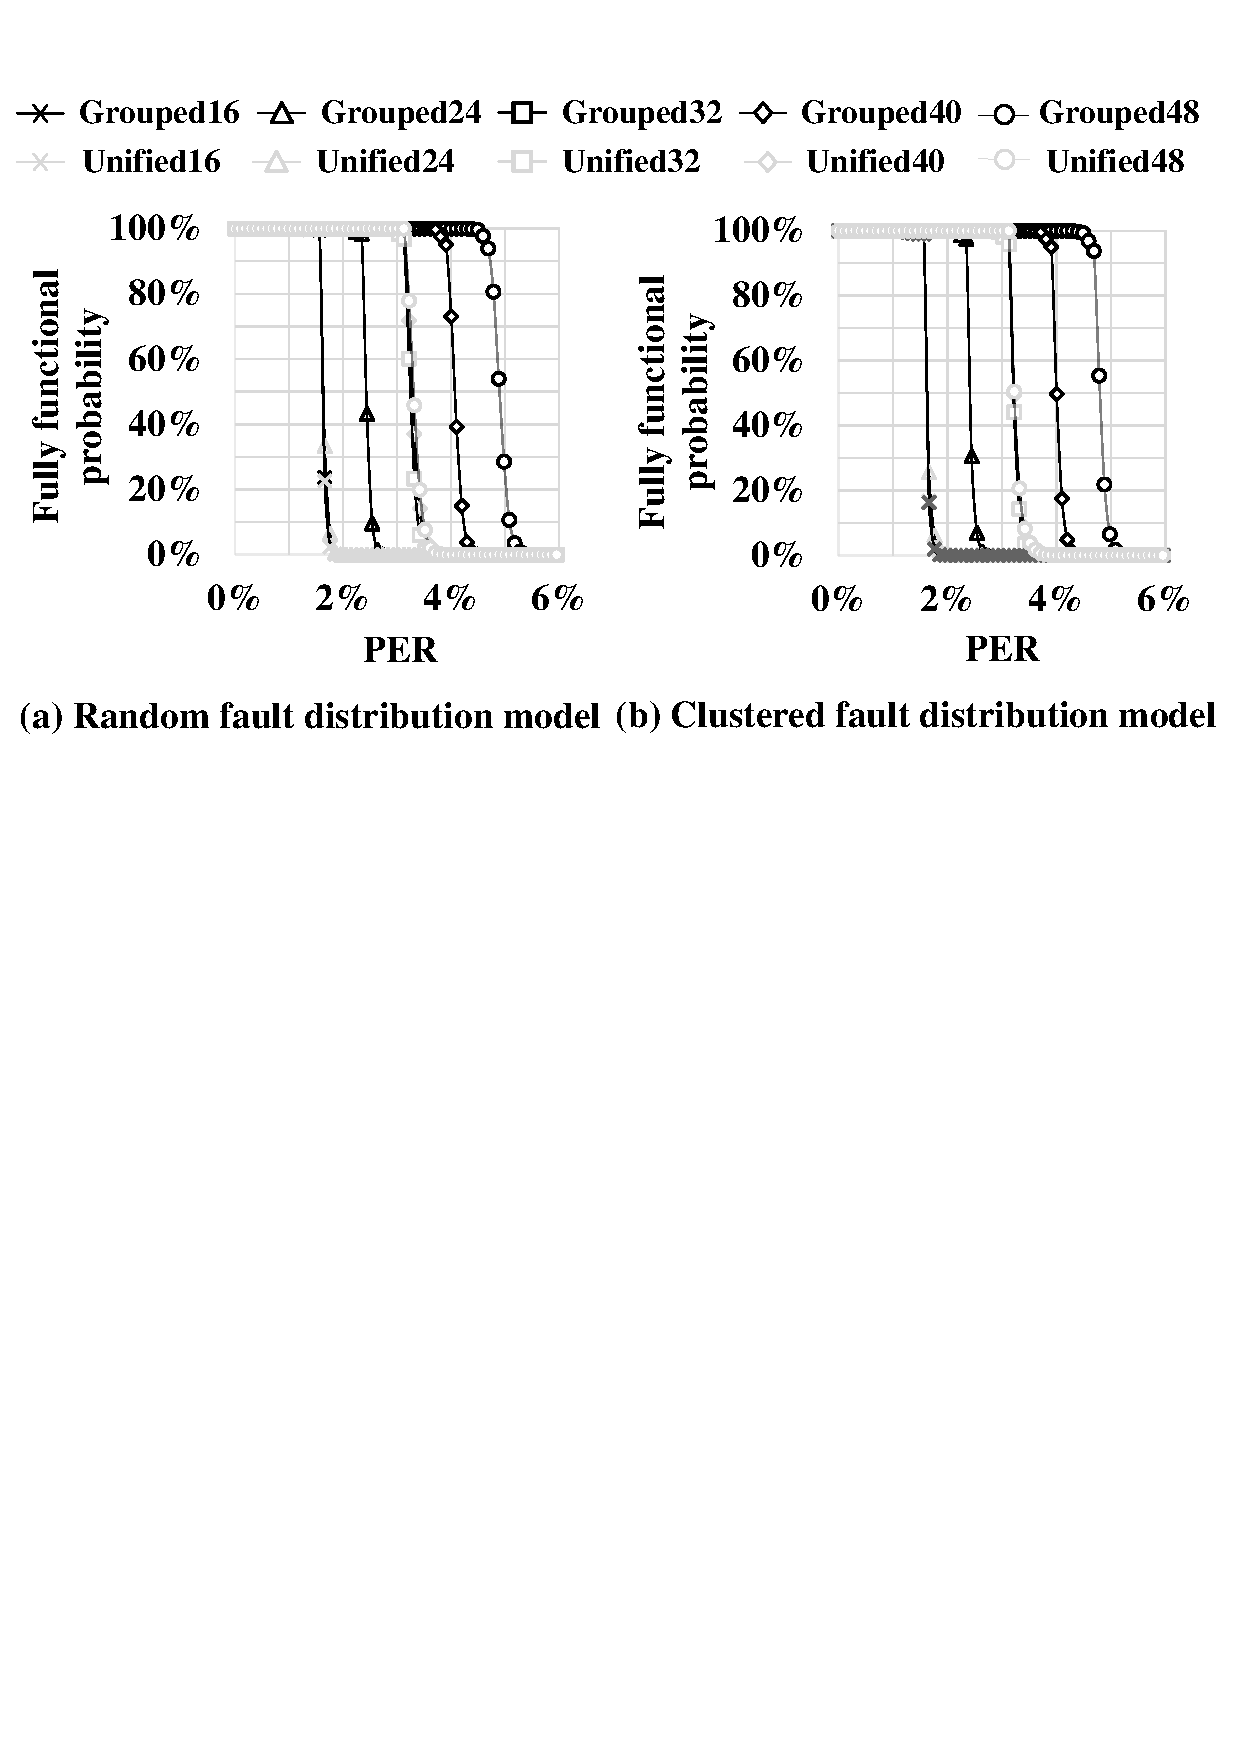
\includegraphics[width=1\linewidth]{images/HyCA-fig15.pdf}}
    \caption{Fully functional probability of the DLAs configured with different DPPU sizes. The DPPUs with both the Unified structure and the Grouped structure are evaluated and compared.}
\label{fig:DPPU}
\vspace{-1.5em}
\end{figure}

\subsubsection{Fault Detection Analysis}
With the proposed fault detection approach, PE faults can be detected at runtime. Since the proposed fault detection module essentially scans all the PEs in the 2-D computing array sequentially, we mainly evaluate the fault detection scanning time under different computing array sizes, and compare the fault detection time to the corresponding neural network processing time. Basically, we want to determine if a runtime persistent fault can be detected before a neural network layer is computed. And we take the percentage of the neural network layers that can be detected during the layer processing as a metric to evaluate the fault detection capability. The experiment result is shown in Figure \ref{detection}. It can be observed that all the faults in the 2-D computing array can be detected during the execution of each neural network layer when the 2-D computing array size is smaller than or equal to $64 \times 64$. When the 2-D computing array size reaches $128 \times 128$, the processing time of some small neural network layers can finish the processing before the fault detection module scan the entire 2-D computing array. In this case, we may have to add more DPPU groups for the fault detection. 

The fault detection module mainly includes a check list buffer (CLB) and some control logic. The CLB is $Col \times W \times 4$ bytes and dominates the chip area, but it is only $Row/(2\times W)$ (i.e. 1/4 when $Row = 32$ and $W = 4$) of the input register file. Thus, the CLB overhead is much smaller than the input register file let alone the redundant PEs. Thereby, the chip area of the fault detection module is negligible.


\begin{table}[]
\setlength{\abovedisplayskip}{3pt}
\setlength{\belowdisplayskip}{3pt}
\centering
\setlength{\tabcolsep}{4mm}
\caption{The proportion of the neural network layers of which the execution time can fully cover the fault detection of the entire 2-D computing array.}
\begin{tabular}{ccccc}
\hline
\hline
 Array Size       & 16$\times$16  & 32$\times$32  & 64$\times$64  & 128$\times$128 \\     \hline
Alexnet & 8/8           & 8/8           & 8/8           & 4/8     \\            
VGG     & 16/16         & 16/16         & 16/16         & 16/16   \\            
YOLO    & 22/22         & 22/22         & 22/22         & 15/22   \\            
Resnet  & 21/21         & 21/21         & 21/21         & 5/21    \\            \hline
\end{tabular}
\label{detection}
\vspace{-1em}
\end{table}

\subsection{Discussion}
The reliability of DLAs is of vital importance to the mission-critical AI applications. Prior redundancy design approaches for the regular computing array such as RR and CR greatly reduce the hardware overhead compared to the classical TMR approaches, but they are rather sensitive to the fault distribution and fail to work especially when the faults are unevenly distributed. To address this problem, we propose a hybrid computing architecture (HyCA) and have a DPPU to recompute all the operations mapped to the faulty PEs in the 2-D computing array. When the number of faulty PEs in the 2-D computing array is less than the DPPU size, HyCA can fully recover the 2-D computing array despite the fault distribution. Even when the fault error rate further increases, DPPU can still be used to repair the most critical PEs first to ensure a large available computing array and minimize the performance penalty. According to our experiments, HyCA outperforms prior redundancy approaches in terms of both the fully functional probability and the computing power under different fault distribution models. In addition, HyCA can also be reused for the fault detection at runtime and the experiment result shows that the entire 2-D computing array can be scanned and detected before a neural network layer completes its execution in most cases.

\section{Online Fault Protection for ReRAM-based Deep Learning}
\subsection{RRamedy Framework Overview}
\subsubsection{Design Goals}
In this section, we analyze the fault models of ReRAM-based edge neural accelerators and elaborate a unified fault detection and network remedy framework for memristor-based deep learning accelerators on the edge. 
\subsubsection{Target Fault Models} 
ReRAM's distinctive characteristics come with reliability concerns. The working mechanism of ReRAM relies on the generation and rupture of the oxygen ions (${{\rm{O}}^{2 - }}$) and oxygen vacancies  (${V_O}$). The stochastic nature of ${V_O}$ makes ReRAM susceptible to many reliability problems \cite{7987496}, including:


{\bf Permanent Faults. } Permanent faults (Hard Faults) of ReRAM cells force the resistance states fixed at high resistance (stuck-at-0 fault) or low resistance (stuck-at-1 fault), which are usually caused by fabrication defects \cite{6725492} and limited endurance. 


{\bf Soft faults.} ReRAM soft faults are mainly resulted from: a) the unavoidable degradation mechanisms and wear-out mechanisms, b) manufacturing defects, especially the imperfect ``electroforming'' process \cite{6957074, Liu:2019:FTN:3287624.3288743}. These soft faults can be observed as retention failures, read disturbance or write disturbance \cite{7879109,8267883}. Even though the ReRAM-based chips have passed the manufacturing test, cells will still suffer from faults/variations during their lifetime, and these effects can be accumulated to result in a data disturbance \cite{8624687}. 

In a nutshell, ReRAM-based edge neural accelerators face both inevitable permanent faults and soft faults in practice.  Permanent faults appear over memory lifetime and cannot be tuned. Soft faults have no permanent corruption on the stored data, but they still have the ability to damage the system. Hence, it is necessary to detect the faults and rescue the system performance from them.  

\subsubsection{Design Requirements}
Here, we outline the design requirements for protecting deep learning accelerators from permanent and soft faults during their lifetime:
\begin{itemize}
    \item Low impact on the performance of DLAs: the proposed solution should have low to no performance overhead on the DLAs, i.e., the fault detection process can be performed in spare time with no impact on the running time of DLAs.

    \item Model fidelity: the accuracy of edge deep learning system cannot be heavily affected. Once faults occurred, the system must detect and diagnose the faults and restore system accuracy instantly.

    \item Fast deployment on the hardware platform: the solution should not introduce modifications on the original architectures and workflows of DLAs.

    \item High generality and reliability: the solution can be practised in different DLAs. The fault detection method should have high fault detection probability. Furthermore, the model retrieving method should alleviate the accuracy degradation and restore the original system prediction accuracy.

\end{itemize}

Next, we describe our proposed framework in detail and show that RRAMedy can apply to any CiM-based edge deep learning accelerators without any constraints on applications or network structures. Meanwhile, our approach did no  modifications on the original workflows of DLAs and the neural network structures. Furthermore, in section \ref{Evaluations}, we show that our proposed adversarial example testing method has superior accuracy on fault detection. Meanwhile, with the model retraining method, the accuracy impact of memristor faults is compensated effectively.  


\begin{figure}
    \centering
    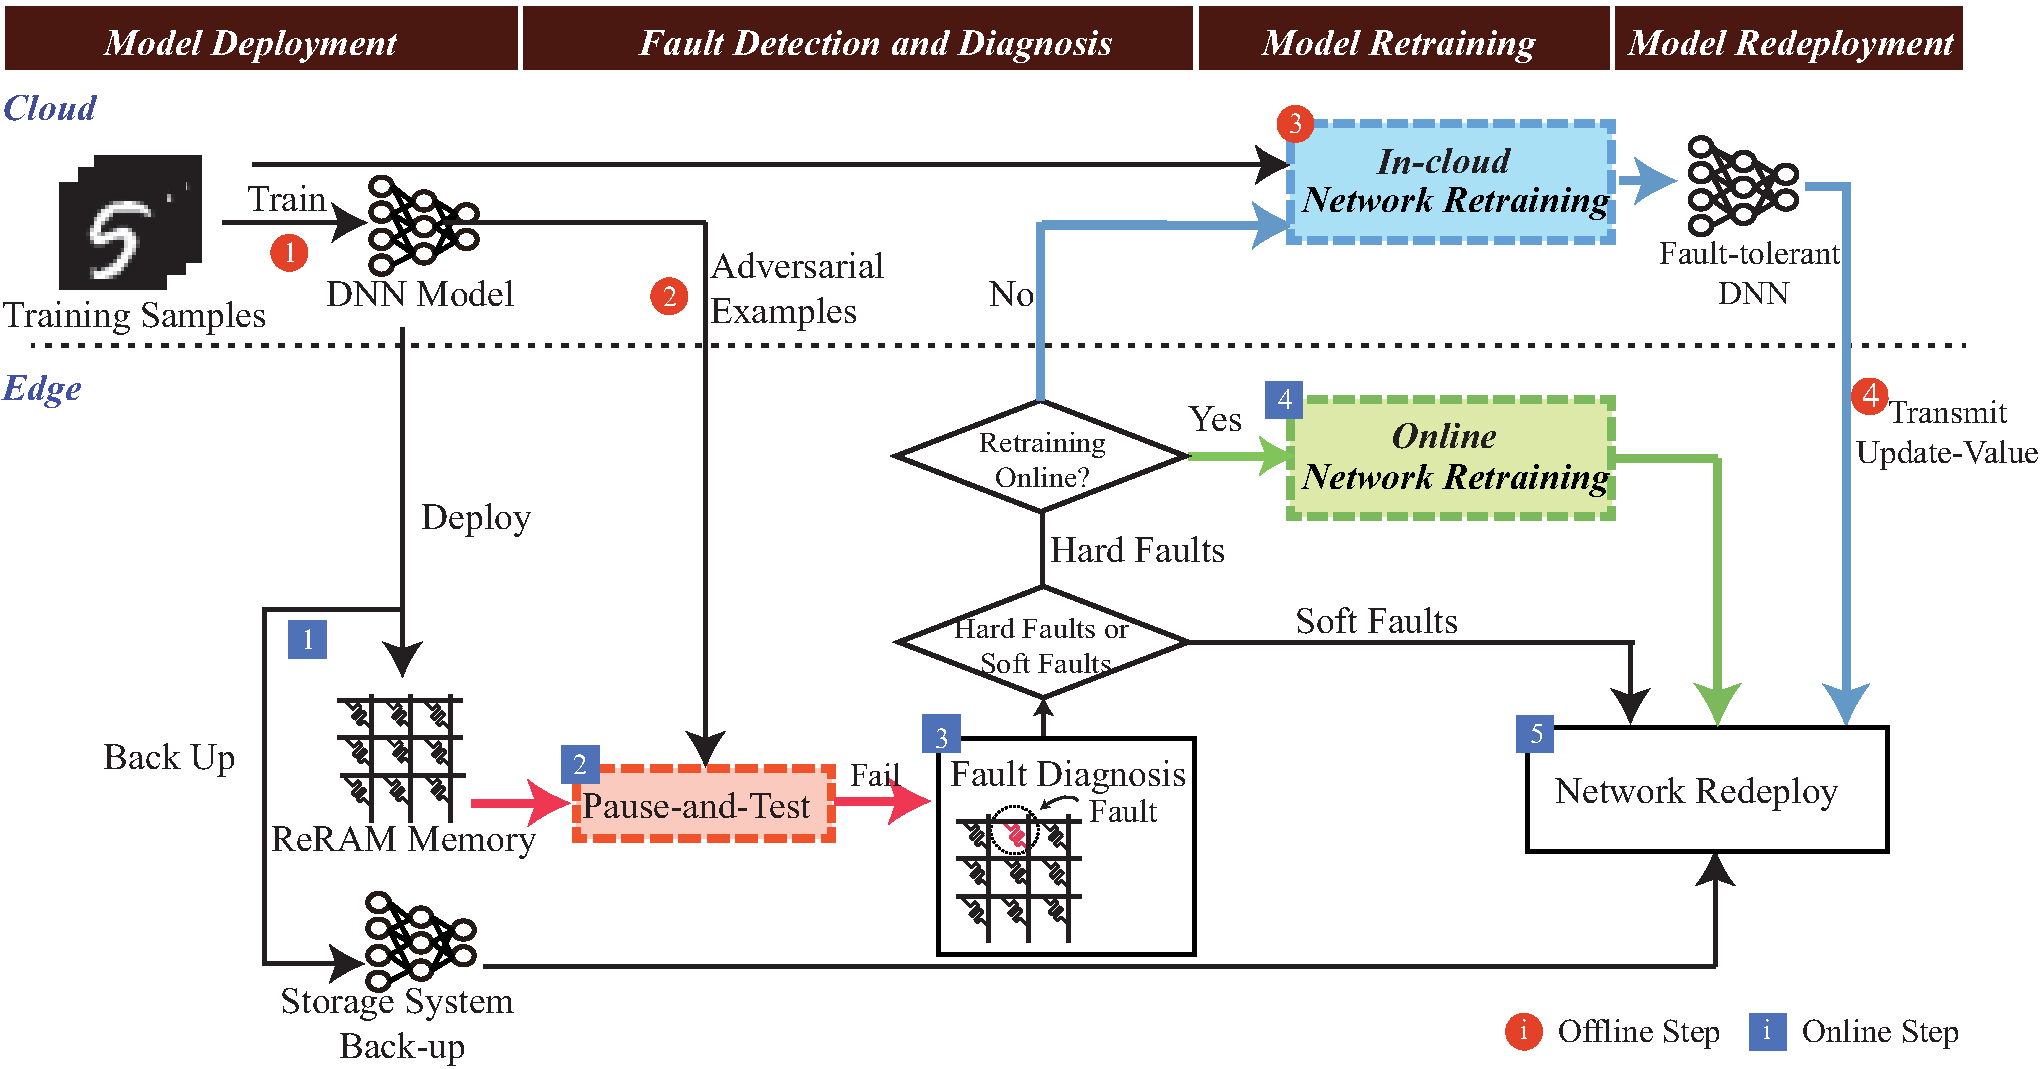
\includegraphics[width=0.8\linewidth]{images/OL-fig3}
    \caption{The global flow of the RRAMedy framework.}
    \label{fig:overview}
    \vspace {-15pt}
\end{figure}

We present the overview of RRAMedy firstly. As illustrated in Fig. \ref{fig:overview}, we model the edge deep learning scenario with two parties, a \emph{cloud server}  and an \emph{edge device} with ReRAM-based memory. The edge device routinely detects its fault occurrence with the proposed Adversarial Example Testing (AET) method. Once a device detects unrepairable faults, it will require updating the current model parameters with a device-specific fault-tolerant model. Here, the updated fault-tolerant model can be trained on either cloud or local edge, according to the edge computational power and the network condition. For devices with limited computational resources, they can ask cloud services for help. The cloud servers will leverage a fault-aware retraining step to generate  fault-tolerant models to maintain the edge system accuracy through the model resilience. Alternatively, for ``powerful" edge devices, they can iteratively adjust neural network parameters to the faults during the online model retraining procedure. 
                                                                            
The RRAMedy framework consists of three primary components, including (1) a fault detector, (2) an in-cloud network retrainer and (3) an online network retrainer. The fault \emph{detector} consists of a ``Pause-and-Test'' (P\&T) mechanism and a ``Fault Diagnosis'' (FD) component.  The P\&T mechanism is periodically invoked to detect system accuracy degradation caused by ReRAM state variations, while the FD component is used for fault diagnosis and generates the corresponding fault distribution. After fault diagnosis,  the framework will choose either the in-cloud network \emph{retrainer} or the online network \emph{retrainer} to finetune the network model for tolerating the irreparable defects. Leveraging the excellent self-recovering capability of neural networks, the faulty network can be retrained with the existence  of unrepairable hard defects. Fig. \ref{fig:overview} demonstrates the general flow of RRAMedy framework that includes four primary phases with five online steps and four offline steps.                                                                                            
                                                                                                
\textbf{Model Deployment.} Firstly, the cloud server trains a network on the cloud (step \circled{1}) and transmits it to the edge device. Then, the edge device deploys the model on the deep learning accelerator for execution and also makes a backup on the storage system (step \rectangle{1}).
                                                                                                        
\textbf{Fault Detection and Diagnosis.} As having addressed, fault detection and diagnosis always bring high overhead. To reduce the overhead, a routinely invoked fault detection mechanism is established on the edge device. As seen in Fig. \ref{fig:overview}, the server generates and selects a set of adversarial examples for fault detection. These generated adversarial examples are transmitted, stored in the storage system of devices (step \circled{2}) and periodically fed into the ReRAM accelerator for the fault detection routine (step \rectangle{2}). The detection results will be further analyzed to instruct the execution of the FD component for accurate fault location (step \rectangle{3}). Specifically, if the ReRAM accelerator fails to generate correct predictions on the adversarial test set, the P\&T component will raise an alarm flag to trigger FD. If there is no permanent fault located, it means the ReRAM accelerator encounters soft faults. The device will refresh the corrupted cells with model back-up (step \rectangle{5}). Otherwise, a permanent fault is found by the FD component, RRAMedy will ask for fault-tolerant training to overcome accuracy losses.
                                                                                                                
\textbf{Model Retraining.} RRAMedy provides two model retraining techniques to recover the recognition accuracy of faulty DNNs, including edge-cloud collaborative fault-masking retraining and in-situ model remedy on the edge. For the edge-cloud collaborative model retraining, the cloud server waits for the edge devices to report their fault distribution. As the fault maps are received, the server will retrain the neural network with the proposed fault-masking method and adaptively adjust the neural network to tolerate the device-specific faults (step \circled{3}). Additionally, we also unleash deep learning retraining services with edge computational power and use the inherent fault tolerance of neural network training algorithms to adapt the network parameters to the faults. Certainly, edge DLA has more strict energy and timing constraints than the cloud. Hence, the online model retraining method leverages the intermediate activations transmitted from the golden models as additional knowledge to assist edge training procedure for faster accuracy recovering (step \rectangle{4}).
                                                                                                                            
                                                                                                                                
\textbf{Model Redeployment.} For the cloud-assistant retraining process,  the server only transmits the quantized weight update values to the edge device to reduce the communication overhead (step \circled{4}). The edge device will then update the cloud-retrained network on its storage system (step \rectangle{5}) and use the updated backup to refresh the ReRAM states to mitigate the fault-induced accuracy degradation. The backup is also used to refresh the soft fault-induced struck cells once detected.
                                                                                                                                        
\subsection{Adversarial Example Testing on the Edge}
It is well-known that the fault detection and location process is time-consuming, which makes it unacceptable to perform periodically, especially for the edge ReRAM expensive to program due to write overhead. Based on this, we pursue to find a more realistic method to capture the fault-induced system behavior failures. Only when the deep learning system is detected with behavior deviations, the FD function will be triggered, which significantly minimizes the system overhead. 
    
The \textbf{Pause-and-Test mechanism} (P\&T) is proposed to periodically analyze the fault existence at the system behavior level. Fig. \ref{fig:ptest} illustrates the high-level view of the P\&T mechanism. It can be described as a function: ${{M}} \to \{ 0,1\} $, that decides whether the neural model ${M}$ is heavily affected by the faults or resistance variations in the ReRAM memory. Unlike traditional systems, which require bit-level comparison to detect system faults, the deep learning system should analyze the output confidence score directly, because the bit-by-bit comparison is unnecessary. Hence, we consider a simple strategy to distinguish the faulty models from normal models: we feed the test benchmark into the edge neural systems and compare the confidence score of the actual model's prediction with the original prediction confidence. The deviations of the original and actual prediction confidence score should be negligible. Once the prediction scores are determined to be heavily different based on the predefined checking rules, the model parameters are likely to be corrupted and the ReRAM memory is most likely suffering from faults or defects. Then, the RRAMedy framework will further diagnose the faults or variations with the FD process.
                        
\begin{figure}
    \centering
    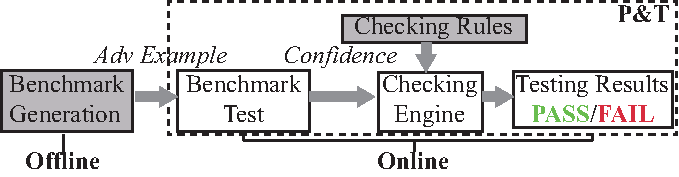
\includegraphics[width=0.9\linewidth]{images/OL-fig4}
    \caption{The overview of Pause-and-Test mechanism (grey components can be adjusted by the cloud servers). }
    \label{fig:ptest}
    \vspace{-10pt}
\end{figure}
                                                                                        
However, neural networks are thought possessing the intrinsic resilience to errors and noises of certain distribution in both inputs and neural weights. Randomly picked input test samples may not activate the faults in ReRAM cells at all, and make the faults escape from software testing, which will increase the risk of fatal failure caused by the latent faults in critical tasks. Thus, we have to propose a more sensitive test method that will activate and detect the faults and elusive cell state variations with high coverage and probability.
                                                                                                
Recently, an adversarial example generating method has been proposed in the deep learning security domain, which is called FGSM (Fast Gradient Sign Method) \cite{43405}. It can be described as:
\begin{equation}
    \label{equ:adv_generate}
    x' = x + \varepsilon  \cdot sign(\nabla xJ(F(x),y))
    %\vspace{-1pt}
\end{equation} 
where the adversarial example $x'$ is generated by adding perturbations to the original sample $x$, as shown in Fig. \ref{fig:advexample}. The perturbations $sign(\nabla xJ(F(x),y))$ are calculated as the sign of the gradient of the model's loss function $J(\cdot,\cdot)$, pushing the original input move towards the direction of the gradient. 
                                                                                                                                        
Though the adversarial examples are used to mislead DNNs originally, we find that they also have great performance on fault detection. Essentially, the adversarial examples are elaborately generated according to the loss gradient, which is on the contrary of the weights update direction. Thus, the weight variations will have a severer impact on the prediction of adversarial examples.  
                                                                                                                                                
To demonstrate the sensitivity of adversarial examples on parameter variations, we conducted an experiment by feeding a normal input and an adversarial input into a normal network and a faulty network respectively. The faulty model is generated by injecting faults on the original model parameters, degrading its classification accuracy from {98.6\%} to {96.8\%}. 
                                                                                                                                                        As illustrated in Fig. \ref{fig:detection-mnist} (a), When we feed a normal sample into the two networks, there is only a {4\%} difference in the top-ranked output confidence scores. But both the normal network and the faulty network predict the normal sample as the same label `0'. However, as shown in Fig. \ref{fig:detection-mnist} (b),  when the network parameters are injected with faults, the output prediction of the adversarial sample totally changes from label `0' to label `8'. This is because that the adversarial examples are generated elaborately according to the loss gradient. Small disturbance on network parameters will result in large deviations on the confidence score. Hence, it is easier to detect subtle faults on edge devices by using adversarial examples.
                                                                                                                                                            
\begin{figure}
    \centering
    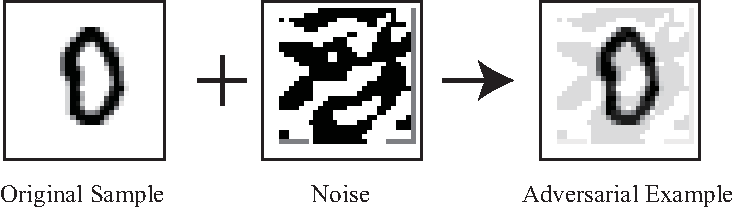
\includegraphics[width=0.7\linewidth]{images/OL-fig5}
    \caption{A demonstration of adversarial example generation.}
    \label{fig:advexample} 
    \vspace {-15pt}
\end{figure}

\begin{figure}[b] 
    \centering
    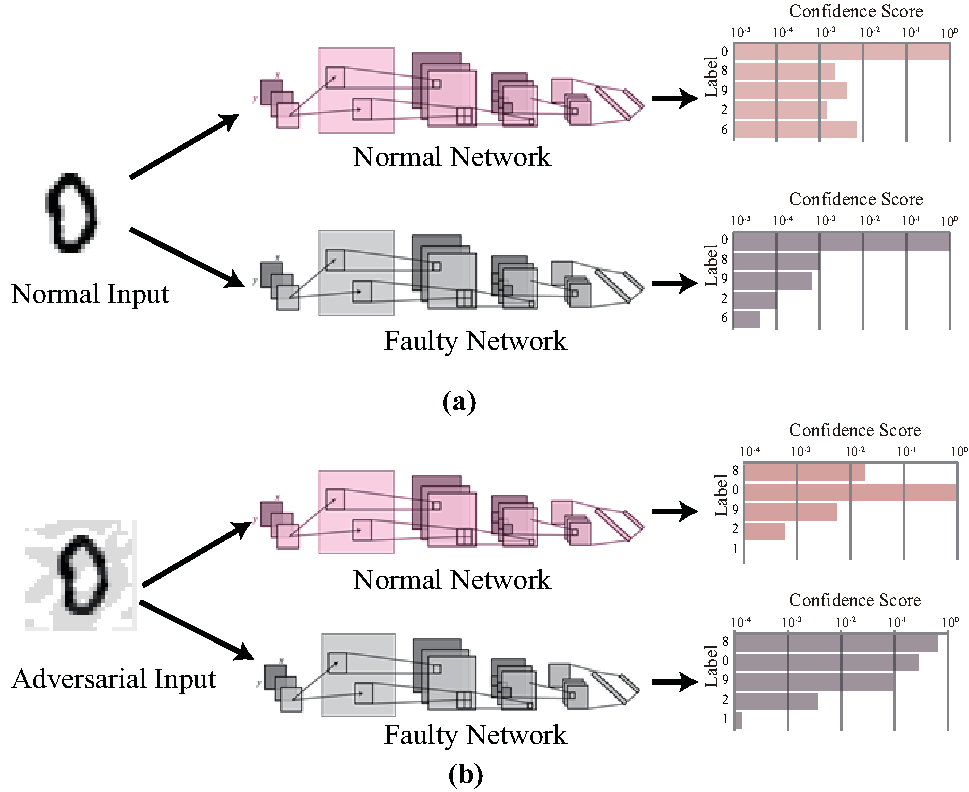
\includegraphics[width=0.8\linewidth]{images/OL-fig6}
    \caption{ The variations of confidence scores (a) when feeding the normal input into the normal network and faulty network and (b) when feeding the adversarial input into the normal network and faulty network.}
    \label{fig:detection-mnist}
\end{figure}
                                                                                                                                                                                                                                                                        
{\bf Fault Diagnosis.} Here, we adopt the March C${^-}$ test algorithm for further fault diagnosis.  Specifically, March C${^-}$ applies a series of read/write operations to a given memristor array by a specific address order and can achieve complete fault coverage by analyzing the fault dictionary \cite{Wang2006VLSI}. March C${^-}$ is denoted as follows:                                                                                                                                                                                                                                                               
\begin{equation}
    \setlength{\abovedisplayskip}{-5pt}
    \setlength{\belowdisplayskip}{-1pt}
    \begin{array}{*{20}{l}}{\rm{March}}\;{{\rm{C}}^ - } - \{  \Updownarrow ({\rm{w0}}); \Uparrow ({\rm{r0}},{\rm{w1}}); \Downarrow ({\rm{r1}},{\rm{w0}}); \\ \qquad \qquad \qquad \Downarrow ({\rm{r0}},{\rm{w1}}) \Downarrow ({\rm{r1}},{\rm{w0}}); \Uparrow (r0);\} 
    \end{array}
\end{equation}
                                                                                                                                                                                                                                                                                                                                
The symbol  '$\Uparrow$' , '$\Downarrow$' and '$\Updownarrow$' denote the order of address sequence. The increasing address direction is represented by the '$\Uparrow$' symbol, and the decreasing address direction is denoted by the  '$\Downarrow$' symbol. The symbol '$\Updownarrow$' is used when the address direction is irrelevant. Besides, '$w0$', '$w1$', '$r0$' and '$r1$' represent the write 0, write 1, read 0 and read 1 operation, respectively. It has been proved that the six March elements in the March C${^-}$ algorithm can detect all the modeled faults \cite{7551274}. Obviously, it requires five read operations and five write operations for each memristor which brings huge time overhead. Considering the limited write endurance of ReRAM, our proposed RRAMedy framework only activates the FD component  when the P\&T mechanism detects the memristor faults, instead of using the March algorithm directly for fault detection. 


\subsection{Fault-masking Retraining on the Cloud}
Once there are unrepairable faults detected on the resource-limited edge devices, cloud servers need to take measures to rescue the system performance from memory faults. Conventional edge-based model retraining solutions have an obvious weakness: the retraining process consumes high hardware resources, making it unpractical to be deployed on the edge device. There are also off-device methods that are carried through model training, but it only focuses on making the network robust to faults, rather than eliminating the impacts of faults \cite{7926952}.  Based on this observation, we explore a cloud-edge collaborative model retraining method. For the {\bf Cloud-Edge Collaborative Method}, the edge device only needs to generate the corresponding fault distribution as a fault-mask in the  ``Fault Detection and Diagnosis'' phase (Fig. \ref{fig:overview}, step \rectangle{3}) and transmit it to the cloud server.  Then, the cloud server will leverage the received fault-mask and apply the proposed {\bf fault-masking retraining method} to adaptively adjust the neural network to tolerate the device-specific faults.
                                        
Unlike previous work that enhances the robustness of network model by using specialized regularization in training, in this work, the goal of the offline model retraining process is to construct a fault-tolerate network $F'(x)$, which can recover the classification accuracy from faulty edge devices. The output of $F'(x)$ is supposed to be close to the original neural network output $F(x)$ , that is:
\begin{equation}
    \forall x:\,\min \Delta (F(x),F'(x))
\end{equation}
                                                                
It has been proven that DNN has the inherent self-recovery capability to relearn the ground truth from the corrupted weights \cite{8013784}.  By applying the Back Propagation (BP) algorithm to update weights, the training model parameters can self-adapt the faults iteration by iteration. The weight updating process can be derived as Equation (\ref{eq:backforward}). However, with the BP algorithm, the weight $ {W_{i}}$ is only tuned to achieve high accuracy without consideration to be adjusted to adapt permanent faults. Hence, to reduce the performance degradation caused by the occurrence of unrepairable permanent faults, we propose to mask the faulty weights which suffer from ``stuck-at'' faults during the model retraining phase. Specifically, the update of weight ${W_i}$ can be described as:
                                                                            
\begin{equation} 
    {W_{i}} \leftarrow Mask({W_{i}} - \eta \frac{{\partial E}}{{\partial {W_{i}}}})
\end{equation}
                                                                                                        
The $Mask$ function is used to fix the faulty bits to their “stuck-at” values during the training phase, according to the received fault-mask. For example, as shown in Fig. \ref{fig:faultmask}, there is a 16-bit-width weight mapped on a row of memristors. However, a stuck-at-1 fault and a stuck-at-0 fault occur on these memristors simultaneously. To ensure the retraining phase can tolerate specific weight deviations, we mask the erroneous bits based on the bit-memristor mapping. When the bit value is mapped on a cell with stuck-at-1 (0) fault, we will fix the value to 1 (0) during the training phase. Therefore, by using the $Mask$-based retraining method on the cloud server, the network itself can compensate for the performance degradation from the error associated with ReRAM faults.
                                                                                                                        
\begin{figure}                                                                                                         
    \centering
    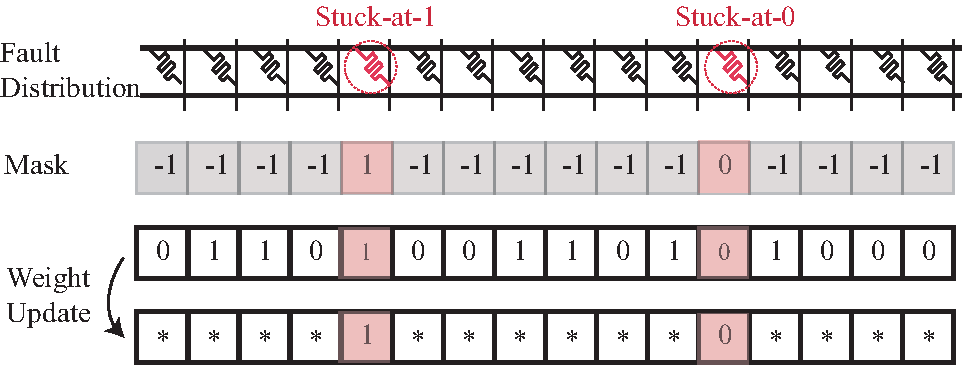
\includegraphics[width=1\linewidth]{images/OL-fig7}
    \caption{Fault-masking retraining.}
    \label{fig:faultmask} 
    \vspace {-15pt}
\end{figure}
                                                                                                                                                                                
Due to communication resource and time constraints, the cloud servers only transmit the gradients to the edge devices, which are also quantized to further reduce the communication overhead, as it is shown that the gradients can be precisely represented by sparse and lower-bit code \cite{NIPS2017_6749}. Then the edge device will use these gradients to update its local model back-ups and refresh the ReRAM states to reduce the fault-induced accuracy degradation.  To rescue from soft faults, the edge device will employ the back-up neural model to refresh the ReRAM arrays. Here, we propose to employ iterative write on the device to make sure the cells are correctly programmed even when the cells are having parametric fluctuations \cite{5482157}.
                                                                                                                                                                
\subsection{In-Situ Model Remedy on the Edge}
In fact, the current situation of implementing DNN retraining phase on the cloud still brings some problems: 

1) Bandwidth competition: if there are numerous edge devices connected to the same network, there exists bandwidth competition between them. Especially when more than one device suffers faults simultaneously, they will request for model update and then exchange information with the cloud, increasing the traffic load of the network.                                                                                                                                                                                                                    
2) Latency:  uploading fault maps to the cloud and offloading updated models from the cloud leaves associated communicational latency which can not be guaranteed to meet the requirements in some time-critical scenarios.

3) Computational pressure on cloud servers: fault-tolerant models are device-specific. Thus, the cloud server will perform the customized DNN training algorithm for every faulty chip, which undoubtedly poses serious challenges to the computational power and the storage resource of cloud servers.

4) Security concern: data transfer between cloud servers and edge devices increases the risk of attack. Even though the cloud server is trusted, edge users still lose absolute control over the transmitted model and data, which gives opportunities for adversaries to perform white-box attacks, black-box attacks and model tampering attacks \cite{10.1145/3287624.3287695}.

5) Reliability concern:  it is a great challenge to guarantee all the devices can connect to the cloud servers. Sometimes, the network connection may be lost. Some devices work in the environment without a network connection. Thus, an online fault-tolerant mechanism should be devised to ensure edge or end devices work normally in anywhere and anytime.
                                                                                                                                                                                                                                                                                                                                    
\begin{figure*} 
    \centering
    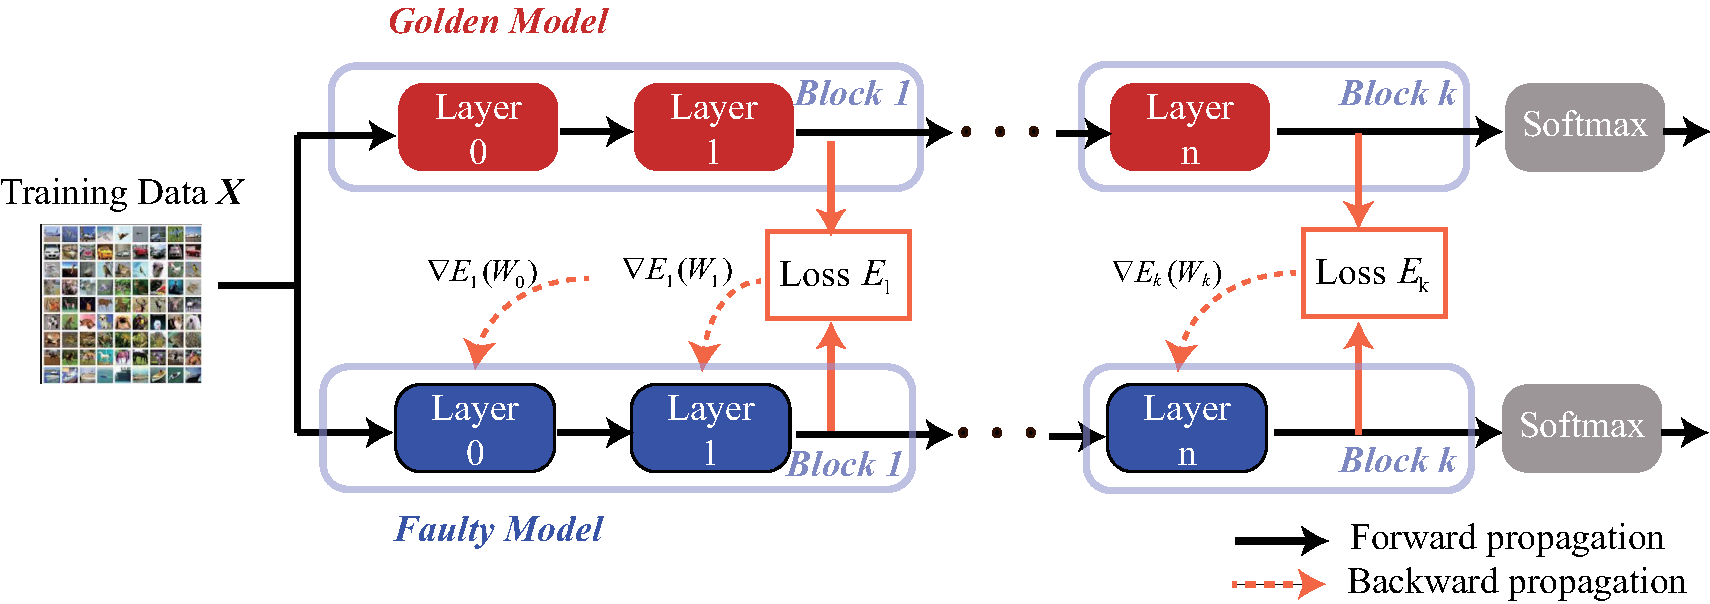
\includegraphics[width=0.75\linewidth]{images/OL-fig8}
    \caption{An overview of our in-situ faulty model retraining mechanism based on intermediate knowledge transfer from the golden model to the faulty model.}
    \label{fig:insitutraining} 
    \vspace{-15pt}
\end{figure*}

To address these concerns, it is desirable to consider implementing retraining-based model-level fault-tolerance on the edge. However, as we all know that, training DNNs is computationally expensive for edge devices. As described in section \ref{Background}, traditional training method uses the BP algorithm which transmits loss gradients from the output layer to the input layer sequentially for weight updates, occupying a significant amount of computational time. Meanwhile, the loss only comes from the final decision without any information extracted from the golden neural network. When DNNs are deep, the final loss is not enough to guide all the weight parameters to coverage quickly. Hence, using the classical training method for online fault-tolerant model retraining will take numerous iterations for weight updates, which not only bring a significant time overhead but also challenge the write endurance of memristors. 
                                                                                                                                                                                                                                                                                                                    
Inspired by these observations, we propose a novel online network retraining algorithm, {\bf Intermediate Knowledge Transfer Retraining (IKTR)}, which introduces the golden model's intermediate represents as additional knowledge to assist the faulty neural networks for accuracy recovering. Herein, the golden model means the ideal model trained on the cloud servers without suffering from any hardware faults. The key idea of IKTR is built upon the popular approach, knowledge distillation (KD) \cite{44873}, which transfers the knowledge from the larger teacher model to a smaller, simplified student model for model compression. At each training iteration, the teacher guides the student network's learning, which achieves significant improvement on network training efficiency. Therefore, we apply this method to the edge fault-tolerant retraining mechanism by treating the golden network as the teacher and the local network as the student. As the golden model preserves rich information on feature extraction, it can greatly help the student network to change its weight values to recover its classification accuracy.

However, the conventional KD method only uses the final output probabilities to optimize the student model, which makes the student model hard to mimic the internal learning behavior of the teacher model. Even though the student is fully optimized with the soft-labels of the teacher network, it may still have very different internal representations, which may affect its  generalization capability  \cite{DBLP:journals/corr/abs-1910-03723}. 

Additionally, it is known that the intermediate representations of DNNs are enriched by the extracted features, which can be better leveraged to assist the student model for behavior imitation \cite{app9101966}. Hence, IKTR leverages the internal information extracted from the golden neural network as additional knowledge to guide the local network fault-tolerant retraining procedure. 

To this end, as shown in Fig. \ref{fig:insitutraining}, IKTR firstly splits the whole neural network into a set of sub-network blocks. In contrast to conventional knowledge transfer, the goal of IKTR is to retrieve the faulty network's accuracy rather than model compression. Hence, the network architecture of the teacher model and the student model is the same. The knowledge will be distilled in the same block from the golden model ($G$) to the local faulty model ($F$) directly. Specifically, we assume that we have a $n$-layer neural network with corresponding weights, $W{\rm{ = [}}{W_0}{\rm{,}} {W_1}{\rm{,}} \cdot  \cdot  \cdot ,{W_{n-1}}{\rm{]}}$. The network is split into $K$ blocks, [$B_1,B_2,\dots,B_K$]. Within each block, there is a set of layers, [$l_1,l_2,\dots,l_m$]. The function of layer $l_m$ can be represented as $f_m({a_{m - 1}};W_m)$. Here, $a_{m-1}$ represents the output activation of layer $l_{m-1}$. The objective of each block in faulty models is to imitate the normal sub-behavior of the golden models.  Thus, we formulate the objective function of each block as follows:

\begin{equation}
    \begin{aligned}
        \begin{split}
            \mathop {\min }  \limits_{{W_F}} \ \Delta ({o_F^k},o_G^k), k \in \{ 1,2, \cdot  \cdot  \cdot ,K\} \\
            s.t. \ {o^k} = {f_{m}}({a_{m - 1}};W_m)\\
        \end{split}
    \end{aligned}
\end{equation}

where $o_F^k$ and $o_G^k$ denote the output activations of the $k$-th block in the faulty network and the golden network, respectively. $l_m$ represents the last layer of the $k$-th block. Unlike the classical BP algorithm, the loss in IKTR is calculated by comparing the faulty model's intermediate representations ($o_F^k$)  with the corresponding golden activations ($o_G^k$). Here, we adopt the Mean-Squared Loss (MSE) as the distillation loss: 

\begin{equation}
    {E_k} = \frac{1}{{s \cdot r}}{(o_G^k - o_F^k)^2}
    \label{equ::MSE}
\end{equation}

\begin{equation}
    s = c \cdot w \cdot h
\end{equation}

wherein, $s$ represents the size of feature maps.  $r$ is the scale ratio. $c$, $w$ and $h$ are the channel counts, width and height of the $o^k$, respectively. By using the MSE loss function for blockwise knowledge distillation, the sub-network training block of the  student network can learn the intermediate feature extraction capacity from the corresponding teacher network block.                                                                              

Meanwhile, as shown in Fig. \ref{fig:insitutraining}, within each block, the loss is still optimized through the conventional BP algorithm. Hence, the loss ${E_k}$ is backward from the top layer to the bottom layer within the $k$-th block. It is worth noting that the optimal solution of the $k$-th block is independent of the other blocks. In other words, the loss ${E_k}$ of block $k$ is only used within the block $k$ and not transmitted to neither block $k-1$ nor block $k+1$. Compared to be trained alone, each sub-network block can learn knowledge directly from the golden model's intermediate activations, which achieves fast network training convergence.

The details of the IKTR algorithm are described in Algorithm \ref{algorithm}. The output of the block $k-1$ is the input of the  block $k$. Considering that errors occurred in the prior block will affect the input of the latter block, the training process is performed from the bottom block to the top block, with the order of (1,2,3,... $K$). Only when the front block is fully optimized, the next block will be trained. During the forward propagation of the blockwise training, the intermediate output activations of layer $m$, $a_{i}^m$, are generated. The output activations of the last layer in each student network's block are used for calculating the difference with the golden model and updating the parameters within the corresponding local training block. Unlike the original BP algorithm, the loss used for weight update of each block is not calculated from the final output as Equation \ref{eq:backforward}, but generated with the blockwise distillation loss. This makes the knowledge directly transfer from the golden model to the faulty model, encouraging the faulty network to simulate the intermediate representations of a golden network. Moreover, within the same block, the training gradient is still calculated with the ``up-bottom" manner (M-1, M-2 ..., 0). Finally, all the training blocks are trained and the parameters are updated to adapt to the unrepairable faults.

\begin{algorithm} 
    \caption{Knowledge Transfer Retraining Algorithm}\label{algorithm}
    \KwIn{faulty weight values $W_0$, previous stored golden feature maps $o_G$,  loss function $L$, training block set $B$}
    \KwOut{updated fault-tolerant weights $W_{i}$}
    \For { $B_k$ {\bf in} Block set \{$B_1,B_2,\dots,B_K$\}}{
        \For{iteration $i = 1,2,...,I$}{
            {\bf Forward propagation:} \\
            Initialize the input of  block $B_k$: $a_0^0 = o^{k-1}$; 
            \For{ layer $m = 1,2,...,M$ in block $B_k$, (M is the number of layers in the block $B_k$) }{
                Compute the intermediate activation of layer $m$:
                $a_{i}^m\leftarrow f_i(a_{i}^{m-1}; W_{i}^m)$\;
                \If{$l_n$ is the last layer of block $B_k$}{
                    $o^k_{F_i} = a_{i}^{n}$;
                }
            } 

            \BlankLine 
            {\bf Backward propagation:}
            Compute the difference between $o^k_G$ and $o^k_{F_i}$: 
            $E^k_i = L(o^k_{F_i},o^k_G)$ (L is calculated according to Eq.(\ref{equ::MSE}));
            
            \For{layer $m=M-1,M-2,...0$ (M is the size of layers in block $B_k$)}{
                Generate gradient $E^m_i$ for layer $m$;  
            }

            \BlankLine 
            {\bf  Parameter update:}
            \For{layer $m = 0,1,2,...,M-1$}{
                $W_i^m\leftarrow Update(W_{i-1}^m,E^m_i)$;
            }
        }
    }
\end{algorithm}

In addition, as IKTR isolates the backpropagation of each block, the computational dependencies are broken. Hence, we improve the IKTR algorithm with a block-wise parallelized training method, {\bf IKTR-P}, where blocks are updated in parallel. As shown in Fig. \ref{fig:paralleltraining}, IKTR updates the latter block only when the front block is fully optimized, which is still a sequential training method. However, for each iteration in IKTR-P, all sub-network training blocks calculate the block losses with the stored golden model's activations and compute the gradients within each block independently and simultaneously. Hence, the backpropagation time of IKTR-P is related to the most computational-complex blocks rather than the whole complexity of the DNN. The evaluations in Section \ref{Evaluations} show that the proposed IKTR-P significantly speeds up the online fault-tolerant training process.

\begin{figure}
    \centering
    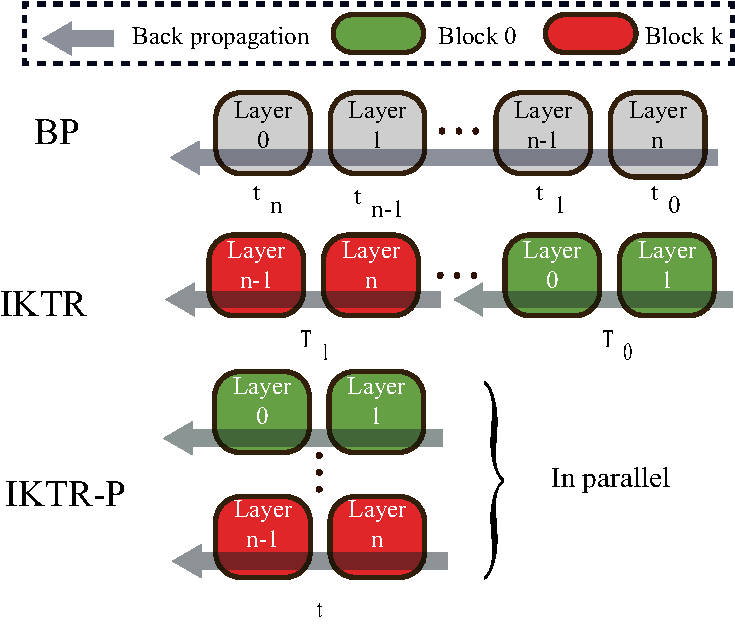
\includegraphics[width=0.75\linewidth]{images/OL-fig9}
    \caption{Illustrations of the different backward propagation approaches including the BP algorithm, the IKTR algorithm, and the IKTR-P algorithm. The rectangles in the same color belong to the same training blocks. The arrow indicates the direction of the loss passing. $t$ represents the relative timestamp in each training iteration. $T$ represents the timestamp in the whole training phase.}
    \label{fig:paralleltraining} 
    \vspace{-10pt}
\end{figure}

\subsection{Experiment Result Analysis}
\subsubsection{Experiment Setup}
{\bf Datasets and Workload.} 
We investigated the effectiveness of RRAMedy on two standard datasets, MNIST and Cifar-10, with three different network architectures, as described in Table \ref{tab:dataset}. The MNIST dataset is used for hand-written digit recognition with 70,000 gray-scale images, wherein 60,000 images are used for training and 10,000 images are testing data. The Cifar-10 dataset consists of 60,000 true-color images of size 3$\times$32$\times$32. The dataset is divided into 50,000 training images and 10,000 test ones. 

\begin{table}[b]
    \centering
    \caption{Benchmarks}
    \label{tab:dataset}
    \begin{tabular}{lcccc}
        \toprule
        Network & Dataset& Classes&Architecture&Accuracy\\
        \midrule
        MLP&MNIST&10&3 FC&0.9616\\
        LeNet&MNIST&10&2 CONV + 2 FC&0.9858\\
        ConvNet-quick&Cifar-10 &10&3 CONV + 2FC&0.745\\
        \bottomrule
    \end{tabular}
\end{table}

{\bf Fault Injection mechanism.} 
To precisely model the impacts of unreliable ReRAM cells on the accuracy of neural networks, we modified the Caffe and TensorFlow framework for fault injection simulation to inject the real-world ReRAM-based faults into ReRAM cells and propagate the errors from the device level to the applications. The faults are injected randomly in the proper network parameters by modifying the 16-bit fixed-point weights in the simulator. For soft faults, we simulated the memristor resistance variations as follows \cite{7926952}:

\begin{equation}
    {w_i} = {w_i}+{{\theta _i}};\theta  \sim (0,{\sigma ^2})
\end{equation}
wherein, the $\sigma$ was set to 0.01 (low), 0.03 (medium) and 0.05 (high) respectively to mimic the resistance drifts in ReRAM cells. 
As for hard faults, we simulated the fault occurrences with both stuck-at-1 (ST1) faults and stuck-at-0 (ST0) faults on SLC ReRAM cells and MLC ReRAM cells respectively. For SLC-ReRAM implementation, when a ReRAM cell suffers from a stuck-at fault, its stored bit-value will be changed to the stuck-at value. As for MLC implementation, we illustrate the fault injection mechanism with 4-level ReRAM MLC cells. When a 4-level MLC ReRAM cell suffers from faults, two adjacent bit-values stored in the same cell will be impacted. For example, when a 4-level MLC ReRAM cell suffers a stuck-at-1 fault, its stored value will be fixed at `11', whatever the value it stored before. Based on this fault injection mechanism, we simulated the occurrence of soft faults and hard faults on ReRAM-based deep learning accelerators.

\subsubsection{Effectiveness of Adversarial Example Testing}
We propose to detect the fault occurrence in deep learning systems with two detection criteria from \cite{Li:2017:UEP:3126908.3126964}, including:

SDC-1: When the top-ranked prediction of the executed DNN is different from the fault-free prediction, we consider that there exist faults in the edge neural accelerator. 

SDC-3\%: The top-ranked confidence score is compared with the ideal execution. If the variations are more than +/- 3\%, we consider that the ReRAM accelerator is faulty.  

To further evaluate the effectiveness of our Adversarial Example-based detection, we did experiments on all the three above-mentioned networks. We tested 100 faulty-models for each network and simulated on both SLC and MLC ReRAM.

Here, we define the {\bf Detection Accuracy (DA)} as a measure of how well the fault-affected neural network can be differentiated from the original model. Specifically, it is defined as the accuracy of the detector when identifying the faulty networks, and can be formulated as:
\begin{equation}
    {\rm{DA = }}\frac{{{\rm{The\ Number\ of\ Identified\ Faulty\ Models}}}}{{{\rm{Total\ Number\ of\ Tested\ Faulty\  Models}}}}
\end{equation}


Furthermore, we try to choose the best adversarial example for fault occurrence detection.  We tested different disturbance $\varepsilon$ (Equation \ref{equ:adv_generate})  to generate adversarial examples. The  $\varepsilon$ used for the AET method in this work is shown in Table \ref{tab:disturbance}.
\begin{table}
    \centering
    \caption{The $\varepsilon$ used in AET method}
    \label{tab:disturbance}
    \begin{tabular}{lccc}
        \toprule
        Network & MLP& LeNet & ConvNet\\
        \midrule
        $\varepsilon$&0.022&0.095&2.1\\
        \bottomrule
    \end{tabular}
\end{table}


\begin{figure*}
    \centering
    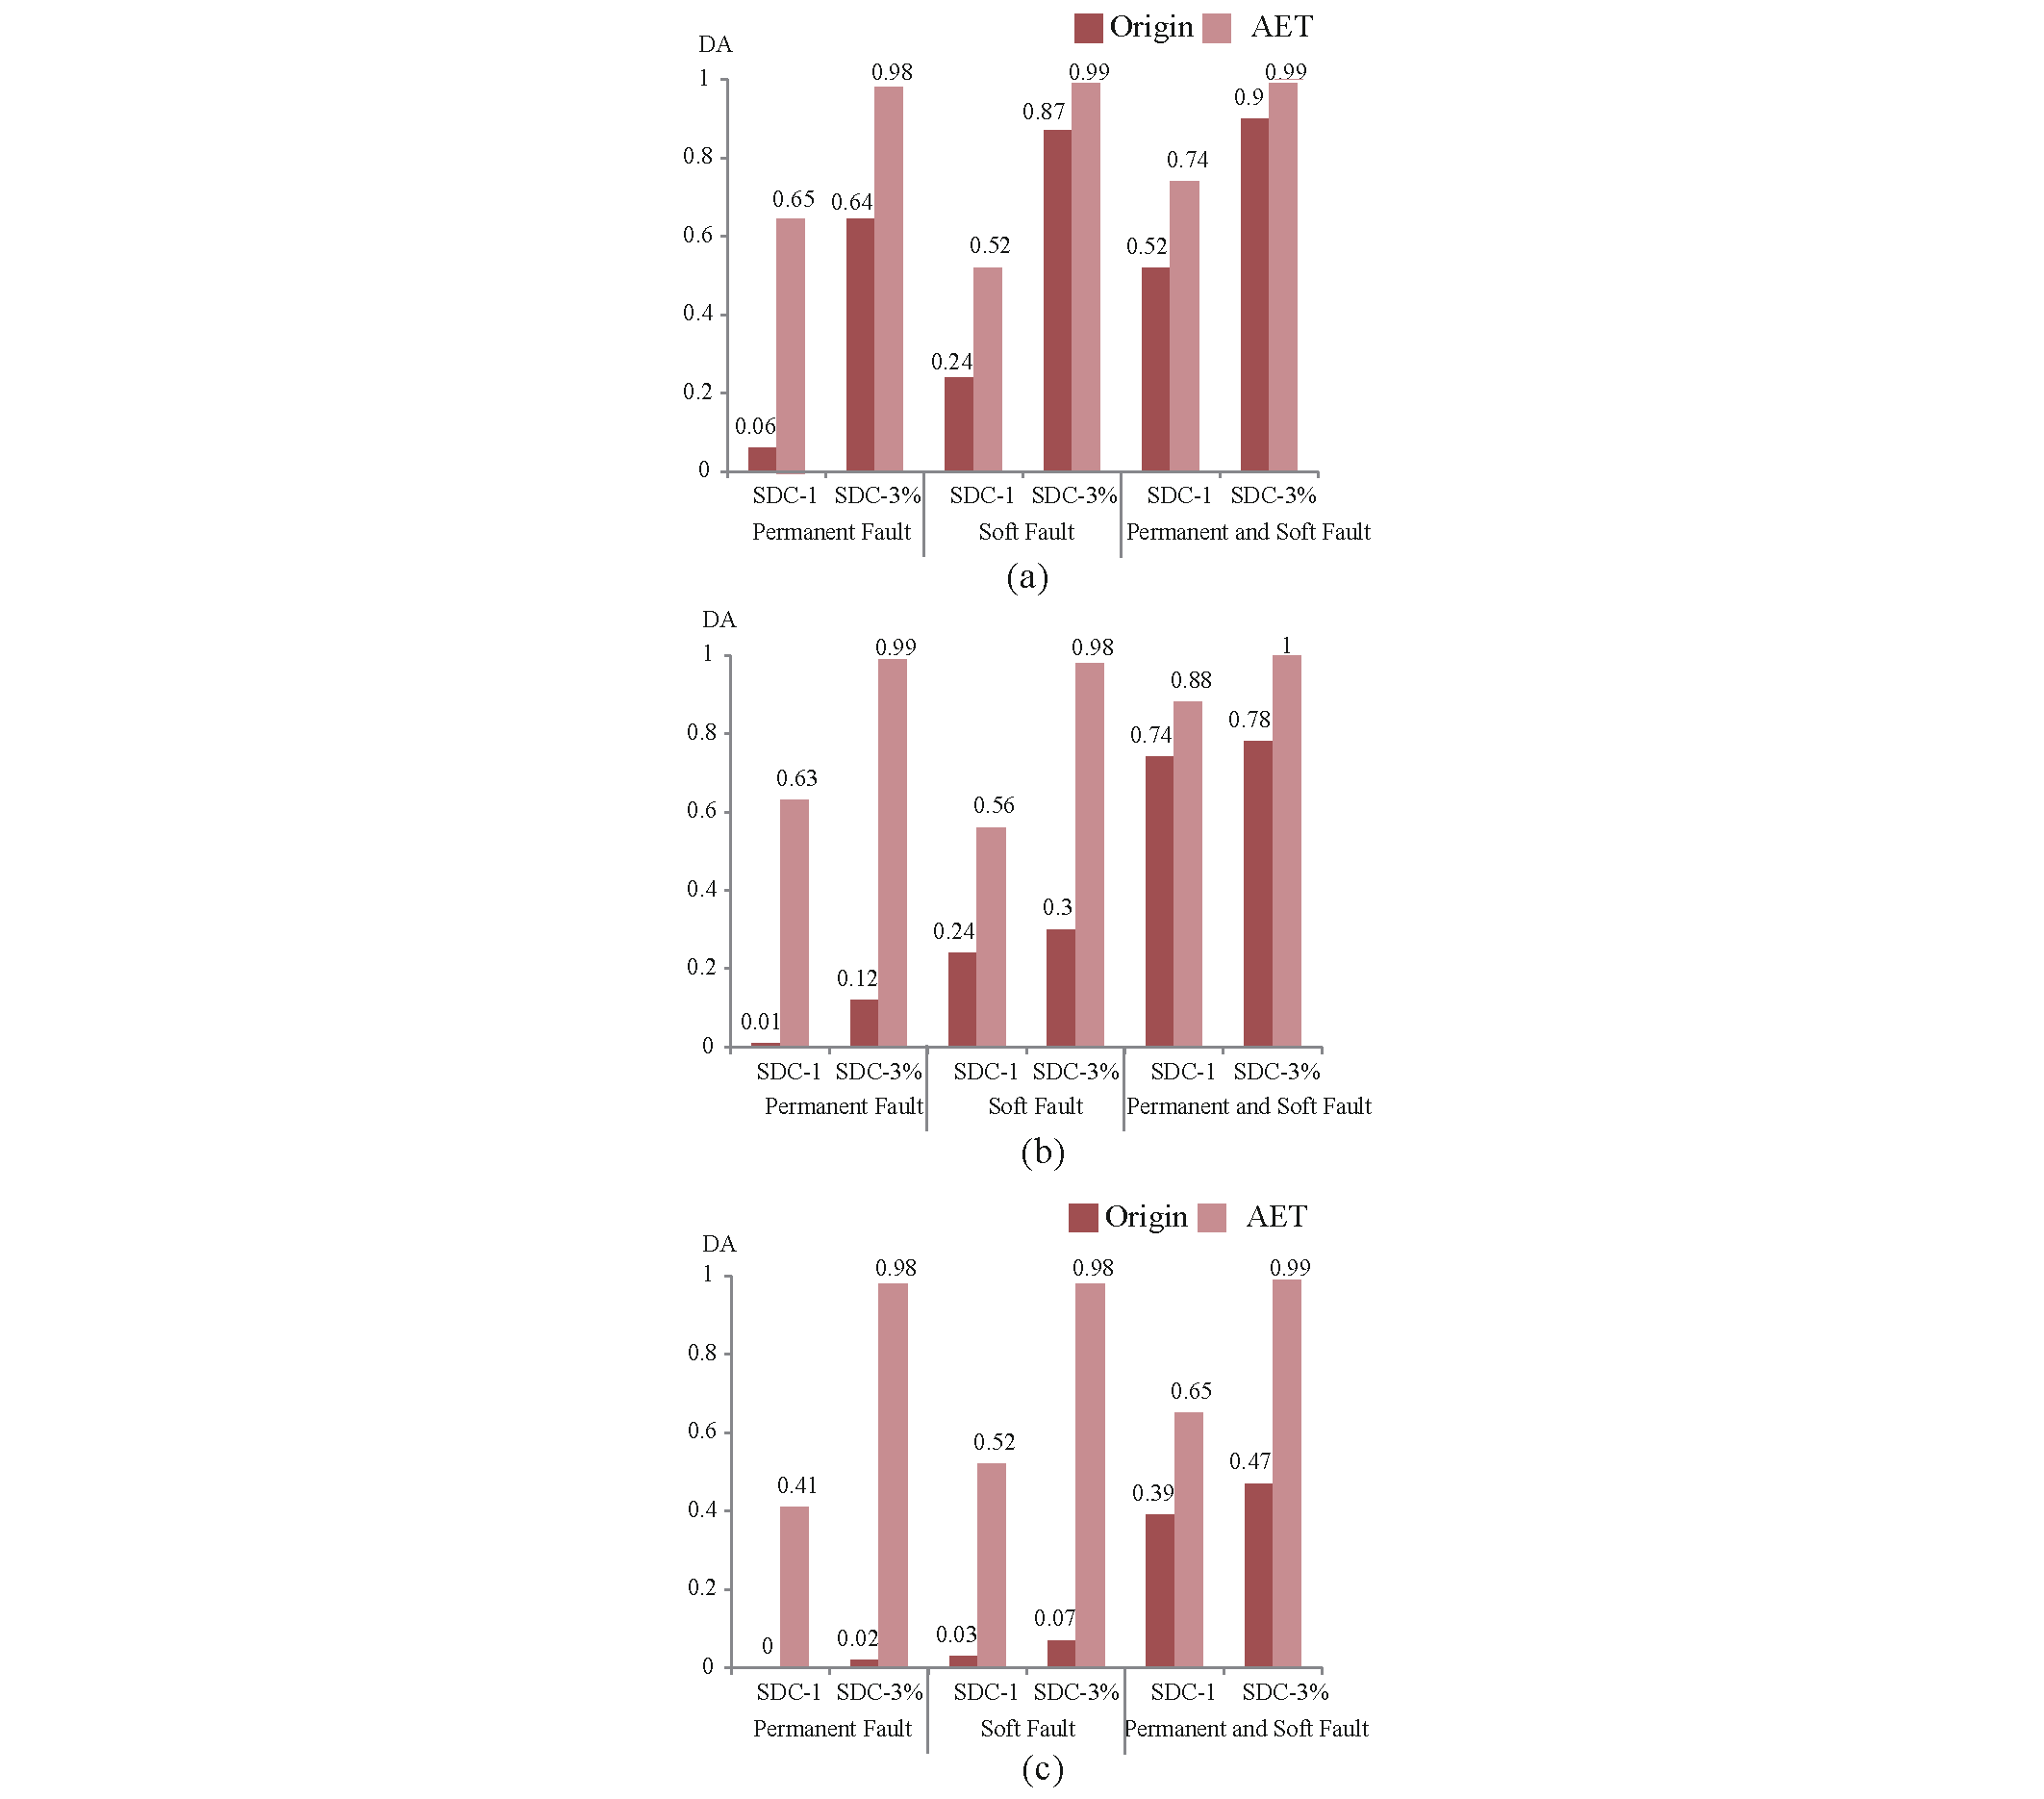
\includegraphics[width=1\linewidth]{images/OL-fig10}
    \vspace{-20pt}
    \caption{Detection accuracy on SLC ReRAM on (a) MLP (b) LeNet (c) ConvNet network with the consideration of only permanent faults; only soft faults and both permanent faults and soft faults occurrence.}
    \label{fig:mnist-slc}
    \vspace{-15pt}
\end{figure*}


(a) Evaluations on SLC ReRAM 

For the SLC mode of ReRAM-based deep learning accelerator,  a 16-bit fixed-point weight needs to be stored in 16 memristors. Considering each cell may suffer from memory faults, we injected both permanent faults and soft faults by randomly modifying bit values within a weight. 
For permanent faults,  five-thousandths of the weight bits are injected with stuck-at faults in LeNet and MLP network. While for the ConvNet network, it is more sensitive to faults. Even if only one-thousandth of weights are faulty,  the classification accuracy drops about 10\% sharply. Since we need to detect faults before they become uncontrolled, we only injected {0.2\textperthousand} faults on ConvNet weight values. As for soft faults, we injected 1\% faults into the MLP and LeNet network, and {0.4\textperthousand} faults into the ConvNet network. Furthermore, we also tested the DAs of the proposed detection method when both permanent faults and soft faults occur simultaneously.

Fig. \ref{fig:mnist-slc} illustrates the DAs of two detection methods on three neural networks. ``Origin'' is the strategy that uses the normal input for fault detection, while ``AET'' uses the proposed AET method. For example, the ``Origin'' method only achieves 64\% detection accuracy on the MLP network for permanent faults, 87\% for soft faults, and 90\% for the existence of both hard and soft faults with the SDC-3\% criterion (Fig. \ref{fig:mnist-slc} (a)). But by using the AET method, the detection accuracy achieves more than 98\% in all the three faulty conditions.  Furthermore, since SDC-1 is a less strict criterion than SDC-3\%, smaller weight deviations can be detected by using SDC-3\%. Hence, we focus on SDC-3\% in the rest of the paper to pursue higher detection accuracy. 

Fig. \ref{fig:mnist-slc} (b) and Fig. \ref{fig:mnist-slc} (c) shows the DAs on convolutional neural networks, LeNet and ConvNet. Obviously,  the AET method outperforms the ``Origin'' test method by more than 22\%. Besides, it is worth noting that when the ReRAM-based deep learning accelerators suffer from both permanent faults and soft faults simultaneously, the AET method achieves more than 99\% detection accuracy.

(b) Evaluations on MLC ReRAM

For the MLC mode of ReRAM-based deep learning accelerator, we consider a $2^2$-level MLC as  \cite{7551379} has used in this section. Each 16-bit weight is distributed to eight ReRAM MLCs. For permanent fault occurrence simulation, the injected faulty rate is as the same as the SLC mode.

For permanent fault detection, as shown in Fig. \ref{fig:mlc-hard}, the ``Origin'' method can hardly differentiate the faulty models from original models, but the AET method achieves more than 97\% detection accuracy with the elaborately generated adversarial example.  

For soft faults detection, as shown in Fig.\ref{fig:mlc-soft}, with larger resistance variations, the DA increases for both three networks. This is because that larger resistance variations will cause severer performance reduction and will lead its output confidence change obviously.  
When considering that both permanent faults and soft faults occur simultaneously, Fig. \ref{fig:mlc-hard-soft} shows that by using AET method, more than 96\% faulty models can be detected on all three networks. Hence, the proposed AET  dramatically achieves high detection accuracy on all the three tested fault occurrence situations.


\begin{figure}
    \centering
    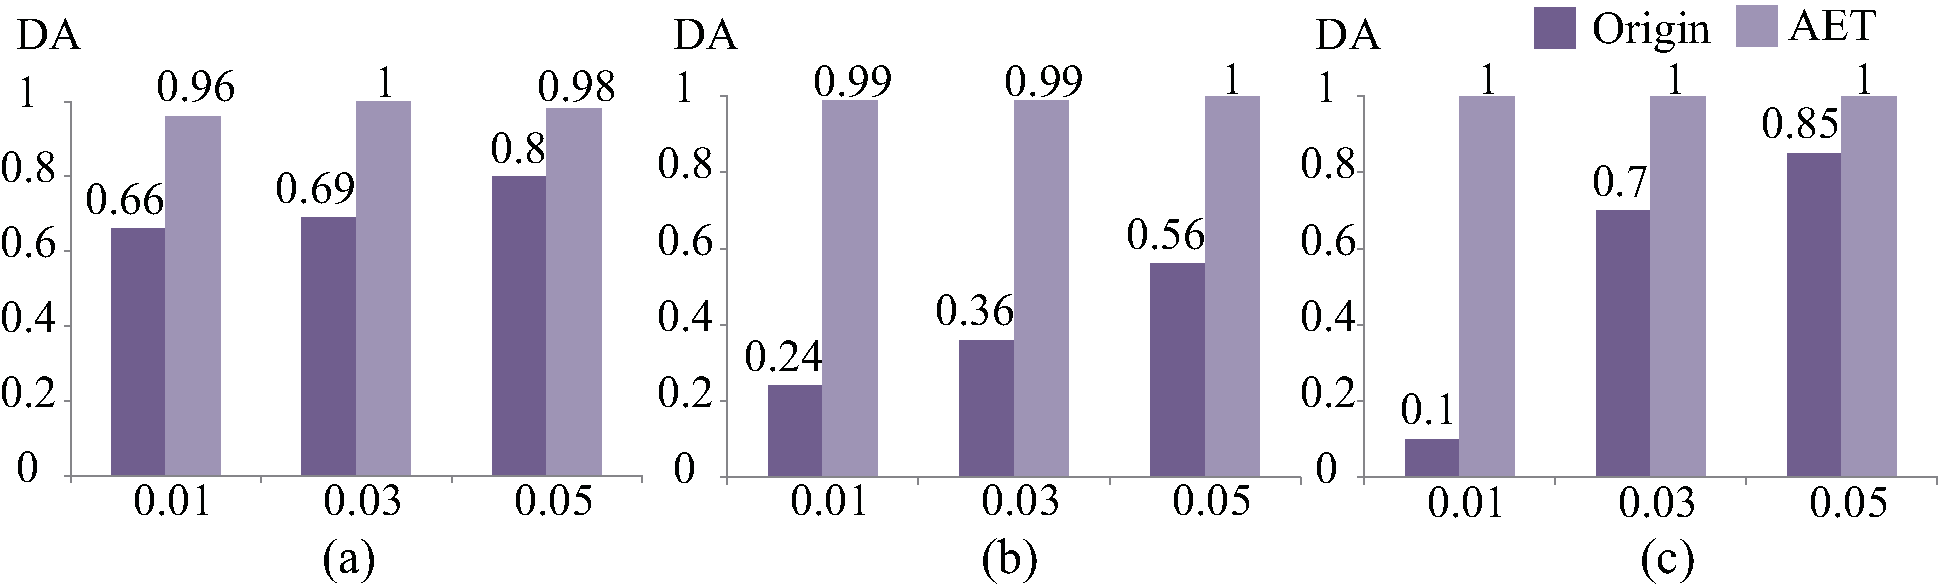
\includegraphics[width=0.75\linewidth]{images/OL-fig11}
    \caption{Permanent fault detection accuracy with the implementation on MLC ReRAM of (a) MLP, (b) LeNet, (c) ConvNet network}
    \label{fig:mlc-hard}
    \vspace{-10pt}
\end{figure}

\begin{figure}
    \centering
    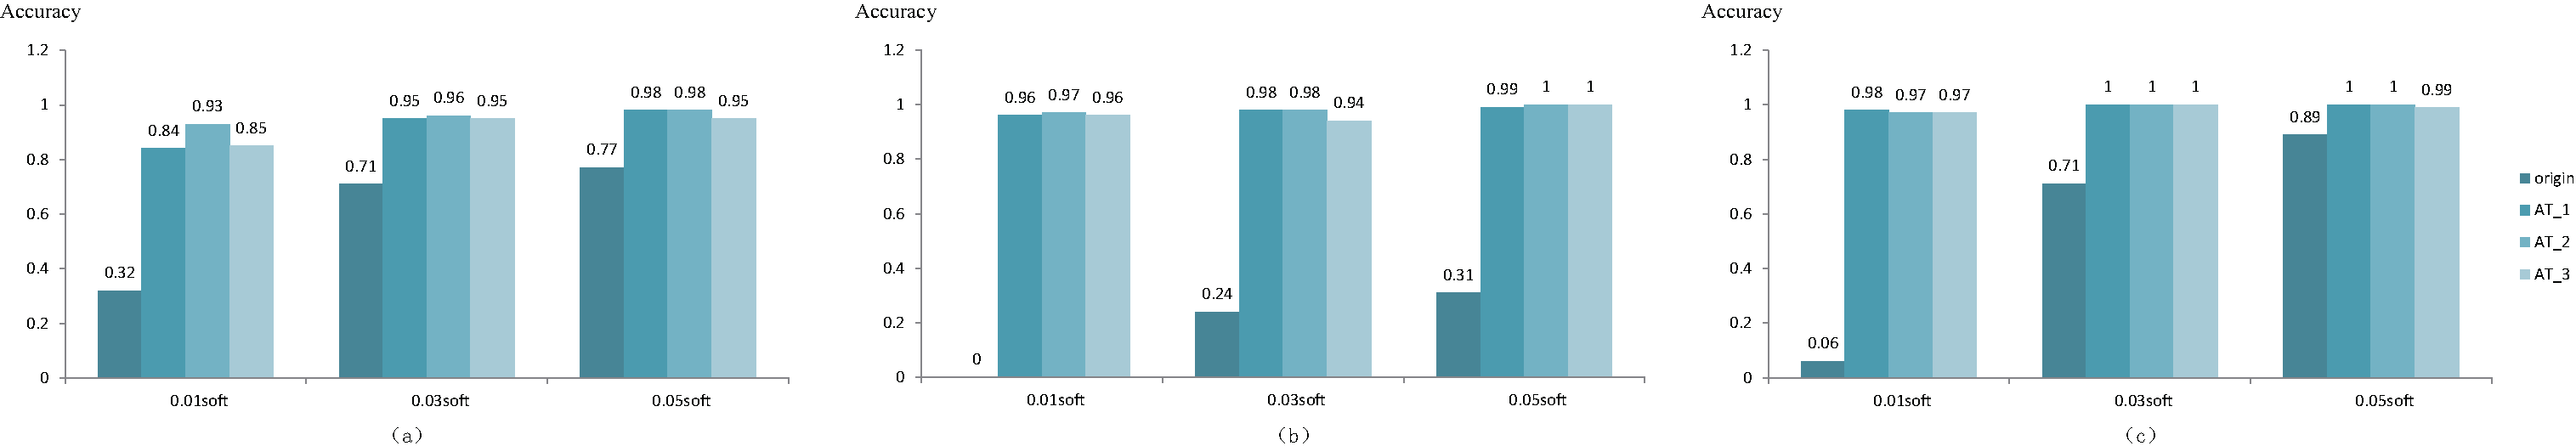
\includegraphics[width=0.75\linewidth]{images/OL-fig12}
    \caption{Soft fault detection accuracy with the implementation on MLC ReRAM of (a) MLP, (b) LeNet, (c) ConvNet network (The X-axis represents the resistance variations $\theta$).}
    \label{fig:mlc-soft}
    \vspace{-20pt}
\end{figure}


\begin{figure}[t]
    \centering
    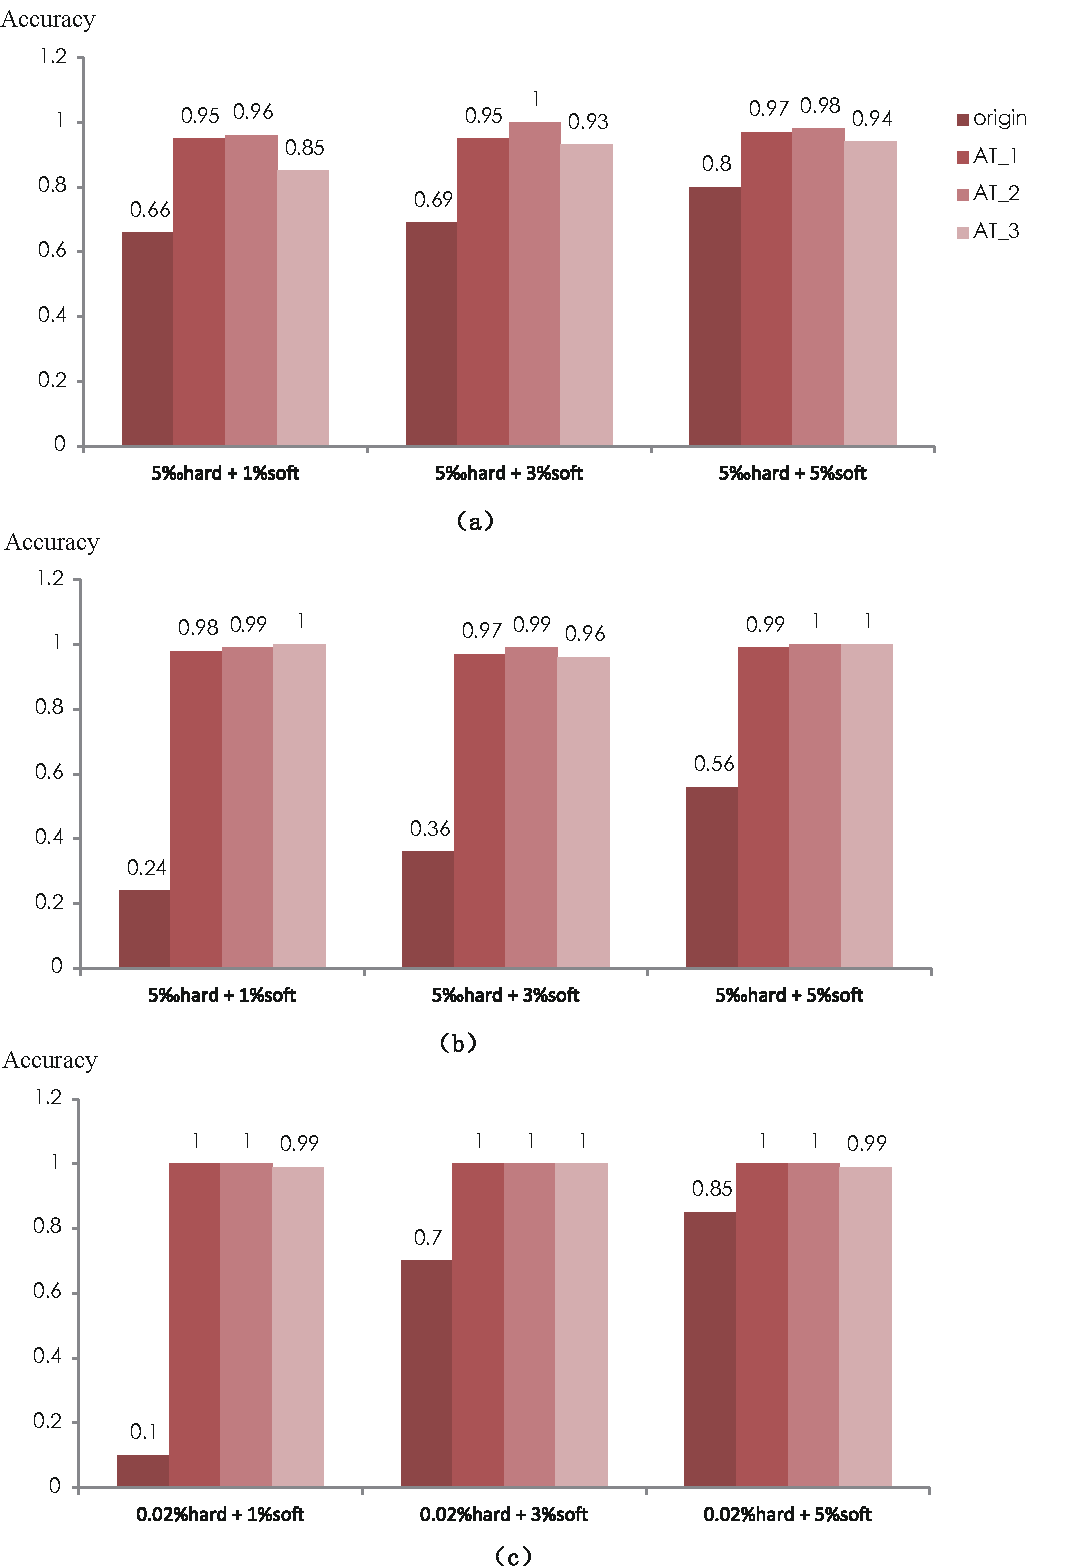
\includegraphics[width=0.75\linewidth]{images/OL-fig13}
    \caption{Fault detection accuracy, considering both permanent faults and soft faults on MLC ReRAM with (a) MLP, (b) LeNet, (c) ConvNet network (The X-axis represents the resistance variations $\theta$).}
    \label{fig:mlc-hard-soft}
\end{figure}


{\bf Performance comparisons.} To compare the performance of our proposed AET-based on-line fault detection and diagnosis method (using AET for fault detection and using March C- for fault diagnosis) with pure March C- algorithm, we executed our benchmarks on a CNN accelerator similar to ISAAC \cite{7551379}, running at 1.2 GHz. The 16-bit fixed-point weight is split into eight 2-bit memristors and the crossbar is composed of 128 * 128  ReRAM cells \cite{Xiangyu2011}. 

The experimental results are described in Fig. \ref{fig:aetperformancecompare}. We observed that when the chip failure rate is 1\%, the proposed AET-based method achieves a speedup from 11.5$\times$ to 91.39$\times$ in comparison with pure March C- algorithm. Since the fully-connected layer has less computational operations but more occupied parameter storage space, for benchmarks with more fully-connected layers, the AET-based method has a higher speed-up ratio. In addition, as the failure rate increases, more fault diagnosis process is executed and the speedup provided by our AET-based fault detection becomes smaller. However, even the chip failure rate is as high as 10\%, our method still achieves more than 5.65$\times$ speedup. Besides, as the write endurance of ReRAM is limited, the proposed AET-based fault detection method saves the memristors from unnecessary memory wear-outs.


\begin{figure}
    \centering
    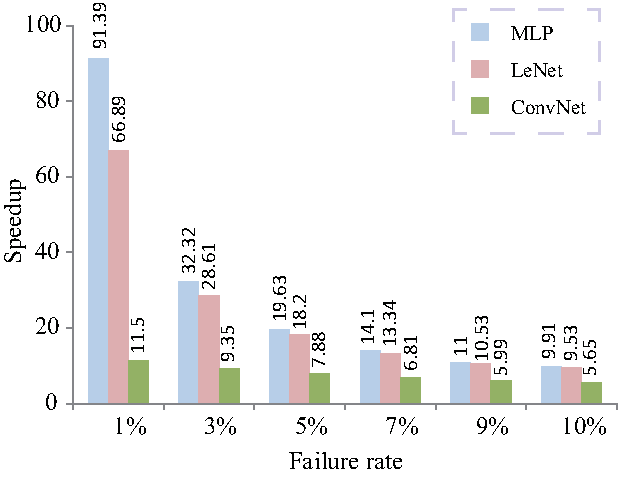
\includegraphics[width=0.8\linewidth]{images/OL-fig14}
    \vspace{-10pt}
    \caption{The performance speedups of our proposed on-line fault detection and diagnosis method.}
    \label{fig:aetperformancecompare}
    \vspace{-15pt}
\end{figure}

\iffalse
\begin{table}
    \centering
    \caption{The performance speedup of AET method}
    \label{tab:time}
    \begin{tabular}{lccc}
        \toprule
        & MLP& LeNet &ConvNet\\
        \midrule
        Speedup&1062$\times$&202$\times$&13$\times$\\
        \bottomrule
    \end{tabular}
\end{table}
\fi

\subsubsection{Effectiveness of Offline Retraining}
\begin{figure}
    \centering
    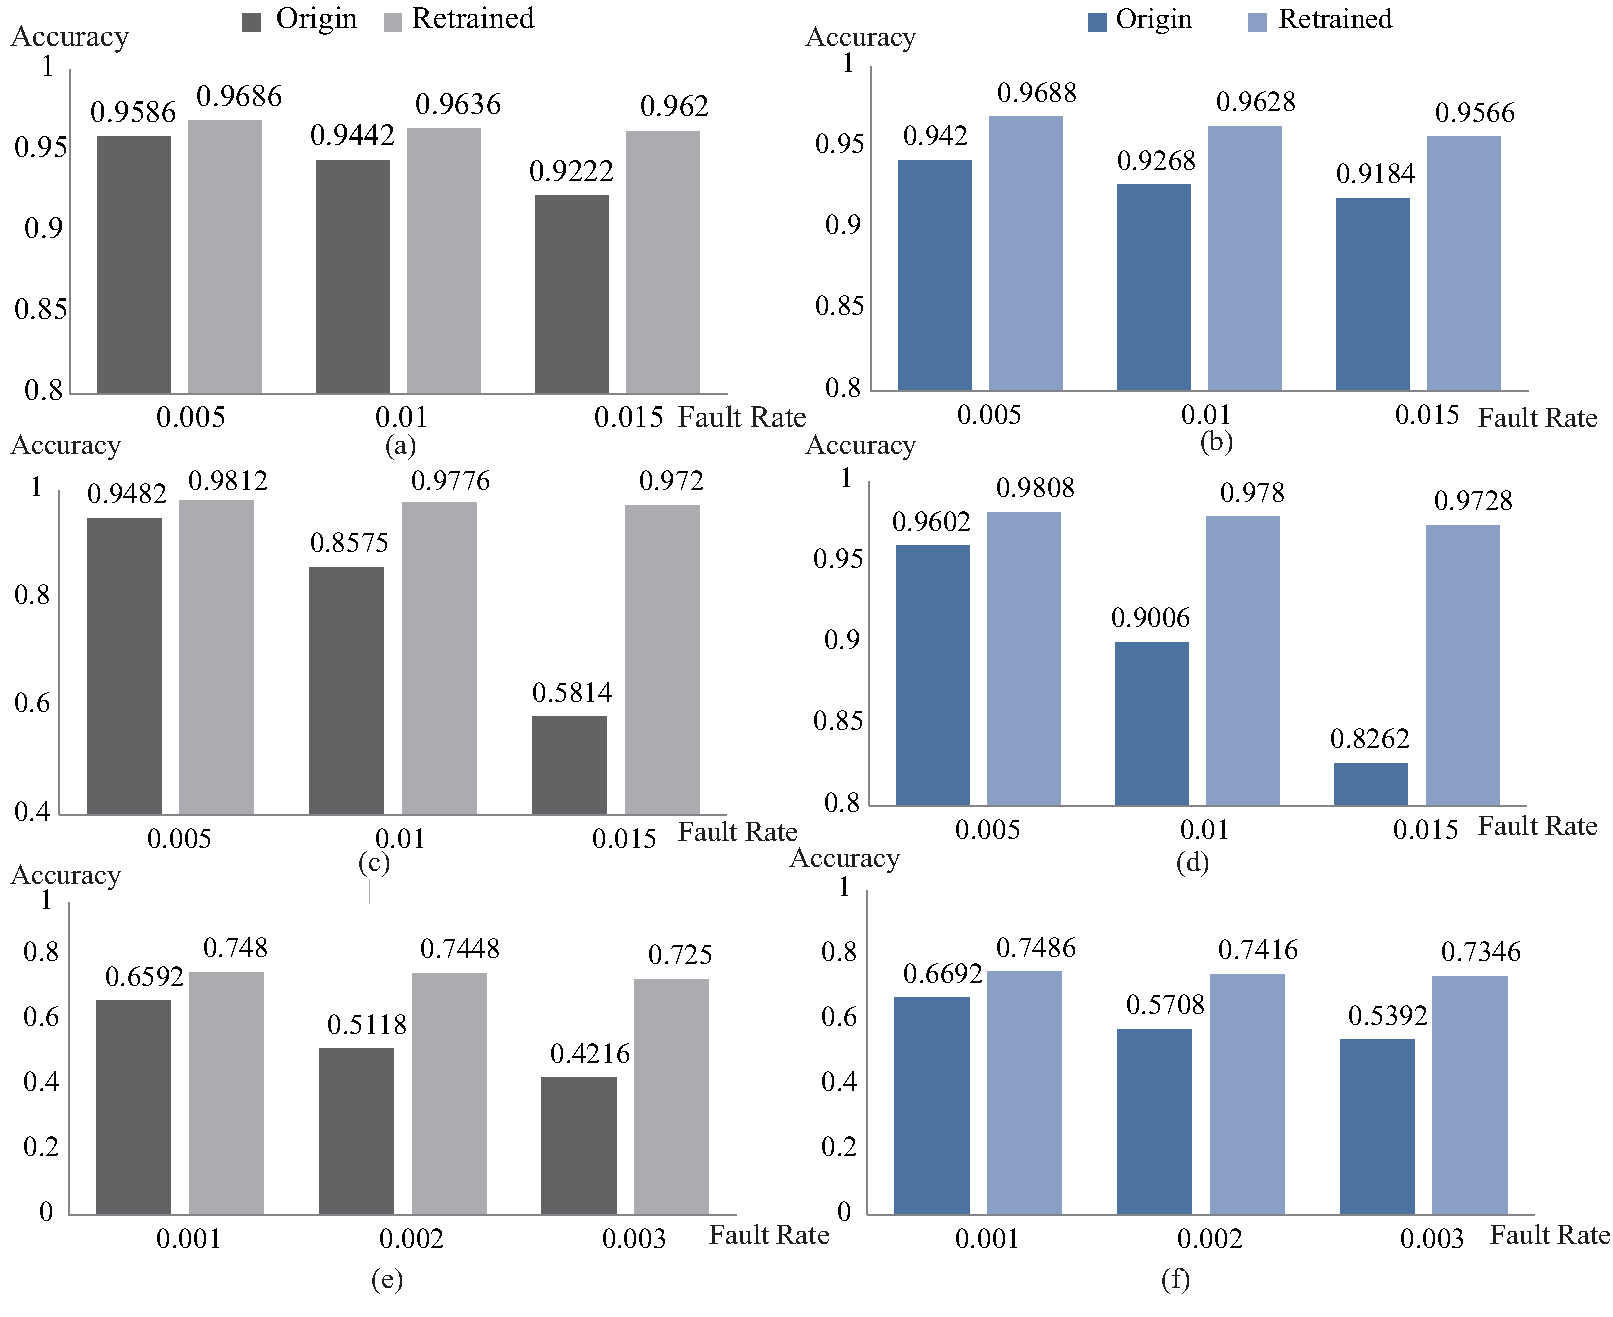
\includegraphics[width=0.8\linewidth]{images/OL-fig15}
    \vspace{-20pt}
    \caption{ Retrieved accuracy of fault-masking training with SLC ReRAM implementation ((a) MLP (c) LeNet (e) ConvNet network) and MLC ReRAM implementation ((b) MLP (d) LeNet (f) ConvNet network)}
    \label{fig:retraining}
    \vspace{-20pt}
\end{figure}


We evaluated the proposed fault-masking training method by simulation-based fault injection. We injected both stuck-at-0 faults and stuck-at-1 faults on each benchmark. The tested fault rate varies from 0.005 to 0.015 on MLP and LeNet, while 0.001 to 0.003 for ConvNet. Fig. \ref{fig:retraining} presents the retrieved accuracy for all the three networks with the SLC ReRAM implementation and the MLC ReRAM implementation respectively. As shown in Fig. \ref{fig:retraining}, the ConvNet is significantly affected by parameter variations. Even though it suffers only one-tenth of injected faults of the other two benchmarks, the accuracy is still dropped by about 8\%. The reason is that the Cifar dataset is more complex than MNIST dataset. Besides, ConvNet only has a small series of layers which makes it has limited fault-tolerance capability. Furthermore, we can conclude from the results that, accuracy can retrieve from heavy system degradation by leveraging the proposed fault-masking retraining method. After retraining, the system performance degradation is less than 2\% on all the three benchmarks.


\subsubsection{Effectiveness of Online Retraining}

\begin{figure*}
    \centering
    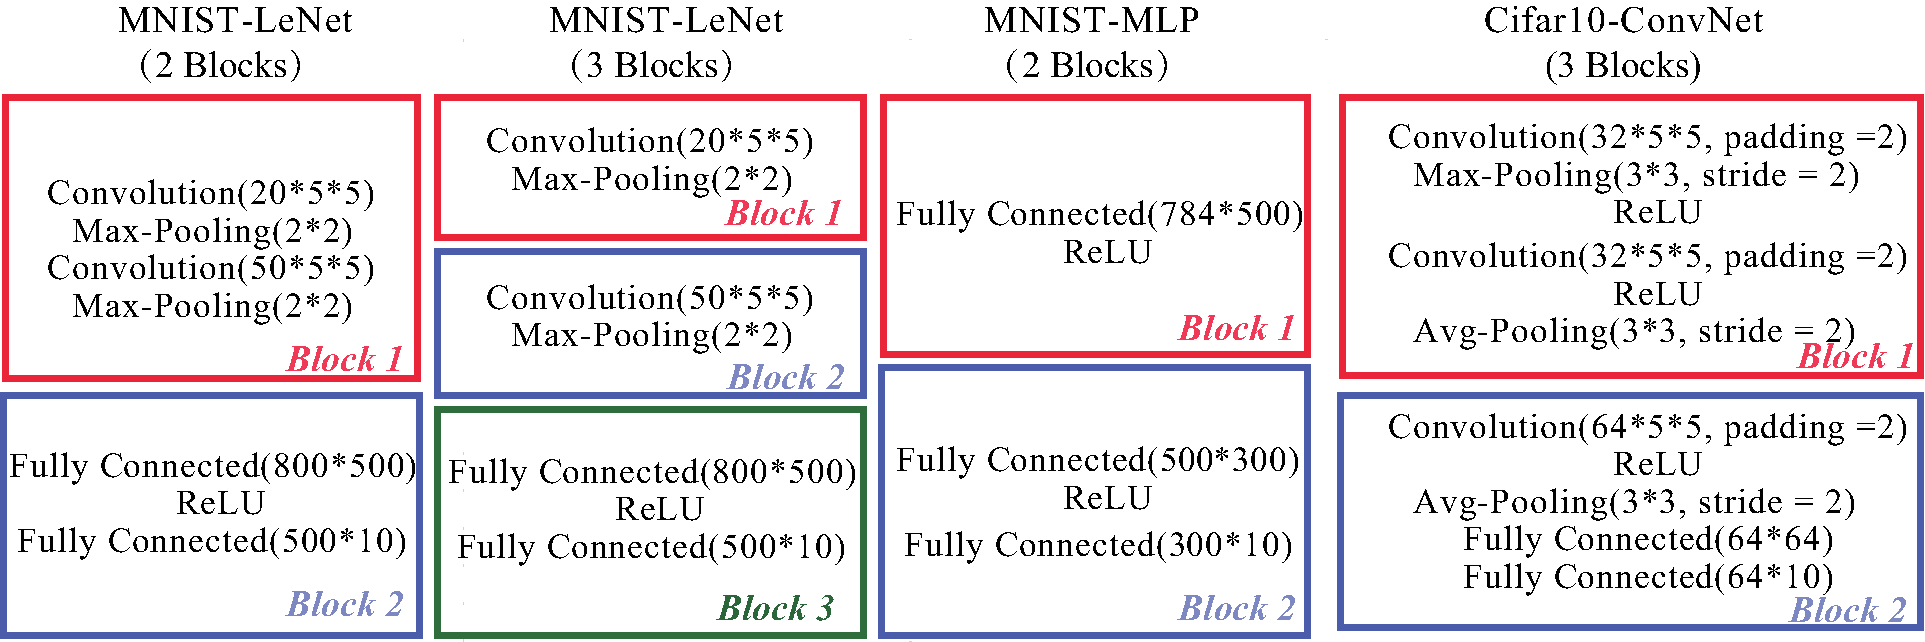
\includegraphics[width=0.85\linewidth]{images/OL-fig16}
    \caption{ The training block partition scheme used in this work. }
    \label{fig:blockpartition}
    \vspace{-15pt}
\end{figure*} 

We evaluated the proposed IKTR-based online retraining method on the aforementioned datasets. The training block partition scheme used in this work is shown in Fig. \ref{fig:blockpartition}. We split the LeNet network, MLP network and ConvNet network into two to three blocks respectively. Meanwhile,  we injected 1\%, 3\% and 1\% hard faults on LeNet, MLP and ConvNet-quick network parameters respectively to simulate both SLC-based faulty DLAs and MLC-based faulty DLAs. 
\begin{table}
    \renewcommand{\arraystretch}{1.3}
    \centering
    \caption{Results of comparing the proposed IKTR and IKTR-P methods with traditional backpropagation algorithm (BP) and knowledge distillation
        algorithm (KD) on three benchmarks (LeNet, MLP, and ConvNet)}
    \label{tab:IKTRresult}
    \begin{tabular}{c|c|c|c|c}
        \hline
        \begin{tabular}[c]{@{}c@{}}Benchmark\\      (Accuracy)\end{tabular}              & \begin{tabular}[c]{@{}c@{}}ReRAM\\      Cell\end{tabular} & Strategy                    & Accuracy        & Speedup    \\ \hline
            \multirow{12}{*}{\begin{tabular}[c]{@{}c@{}}LeNet\\      (0.9881)\end{tabular}}          & \multirow{7}{*}{SLC} & Faulty model     & 0.8027   & -       \\
                &                      & Baseline-BP      & 0.9772   & 1x      \\
        &                      & Baseline-KD      & 0.9853   & 1.25x   \\
        &                      & IKTR(2 blocks)   & 0.9856   & 2.5x    \\
        &                      & IKTR-P(2 blocks) & 0.9856   & 2.83x   \\
        &                      & IKTR(3 blocks)   & 0.9863   & 2.5x    \\
        &                      & IKTR-P(3 blocks) & 0.9856   & 3.13x   \\ \cline{2-5} 
        & \multirow{7}{*}{MLC} & Faulty model     & 0.7457   & -       \\
        &                      & Baseline-BP      & 0.9835   & 1x      \\
        &                      & Baseline-KD      & 0.9845   & 2x      \\
        &                      & IKTR(2 blocks)   & 0.9851   & 2x      \\
        &                      & IKTR-P(2 blocks) & 0.9853   & 2.27x   \\
        &                      & IKTR(3 blocks)   & 0.9854   & 2x      \\
        &                      & IKTR-P(3 blocks) & 0.9854   & 3.34x   \\ \hline
        \multirow{12}{*}{\begin{tabular}[c]{@{}c@{}}MLP\\      (0.9833)\end{tabular}}             & \multirow{5}{*}{SLC} & Faulty model     & 0.8029   & -       \\
            &                      & Baseline-BP      & 0.9623   & 1x      \\
        &                      & Baseline-KD      & 0.9762   & 3x      \\
        &                      & IKTR(2 blocks)   & 0.9771   & 6x      \\
        &                      & IKTR-P(2 blocks) & 0.9770   & 7.38x   \\ \cline{2-5} 
        & \multirow{5}{*}{MLC} & Faulty model     & 0.7909   & -       \\
        &                      & Baseline-BP      & 0.9621   & 1x      \\
        &                      & Baseline-KD      & 0.9743    & 2.5x   \\
        &                      & IKTR(2 blocks)   & 0.9761   & 5x     \\
        &                      & IKTR-P(2 blocks) & 0.9758   & 6.15x   \\ \hline
        \multirow{10}{*}{\begin{tabular}[c]{@{}c@{}}ConvNet\\      (0.7698)\end{tabular}}        & \multirow{5}{*}{SLC} & Faulty model     & 0.4379   & -       \\
            &                      & Baseline-BP      & 0.7248   & 1x      \\
            &                      & Baseline-KD      & 0.7424   & 1.25x   \\
        &                      & IKTR(2 blocks)   & 0.766   & 1.5x    \\
        &                      & IKTR-P(2 blocks) & 0.764   & 1.83x   \\ \cline{2-5} 
        & \multirow{5}{*}{MLC} & Faulty model     & 0.3156   & -       \\
        &                      & Baseline-BP      & 0.7137   & 1x      \\
        &                      & Baseline-KD      & 0.7464   & 1.5x    \\
        &                      & IKTR(2 blocks)   & 0.7511   & 1.5x    \\
        &                      & IKTR-P(2 blocks) & 0.7525   & 2.3x    \\ \hline 
    \end{tabular}
    \vspace{-20pt}
\end{table}

(a) Performance comparisons


The comparisons of the recovered model accuracies and performance speedups between traditional backward propagation (BP) algorithm, knowledge distillation (KD), IKTR and IKTR-P are depicted in Table \ref{tab:IKTRresult}.
Several observations can be seen as follows. Firstly, as depicted in Table \ref{tab:IKTRresult}, all the KD, IKTR and IKTR-P methods can restore the accuracy of faulty neural networks from up to {43\%} accuracy degradation and achieve more than 1.25$\times$ training speedups over traditional BP algorithm. This is because that all these three methods leverage knowledge from the well-trained golden teacher model to make the faulty model mimic the behavior of the golden model. Secondly, the proposed IKTR-based algorithm
still outperforms the traditional KD algorithm. This is because that the KD algorithm only provides the soft labels (output probabilities) to optimize the student model, it is hard for the student faulty model to learn the intermediate behavior of the golden model, especially when the network
becomes deeper. Considering that the internal layers of a neural network has extracted rich information. The IKTR-based method splits the network into small blocks, making each training block locally learn the internal representations from the golden teacher model. Furthermore, the IKTR and IKTR-P methods enable a direct fine-tuning, which avoids a sequential backpropagation through network and consumes few epochs for block-wise network training, further improving the training convergence speed. Thirdly, the proposed IKTR-P method breaks the sequential retraining process and enables parallel block-wise training. Each block trains independently and simultaneously, further accelerating the online retraining procedure.

(b) Analysis of the impact of the number of training blocks
To investigate the performance speedups with different block numbers of IKTR-based online remedy methods, we validated the proposed IKTR method with both two sub-blocks partitioning and three sub-blocks partitioning on the LeNet network. As we can see from Table \ref{tab:IKTRresult}, when we split the LeNet network into three blocks, it achieves higher retrieved accuracy than two sub-blocks partitioned IKTR-based training. The improvement can be explained by the fact that the IKTR method divides the highly complex optimization problem into several simpler subproblems. When the number of sub-blocks increases, each training block becomes smaller and easier to be trained. Meanwhile, with more training blocks partitioned, more internal knowledge is transferred to the faulty student neural network, which helps it to mimic the behavior of the golden model. However, the size of the partitioned sub-network training block cannot be too small, which may lead to over-fitting and decrease the retrieved accuracy. Furthermore, more training blocks achieve additional speedup through parallel training (IKTR-P). It can be seen from Table \ref{tab:IKTRresult}, for the Lenet network, three-block partitioned IKTR-P training outperforms the two-block partitioned IKTR-P training with 1.2$\times$ speedup on average. The reason is that, blocks are trained separately in parallel in IKTR-P. Hence, the runtime for IKTR-P depends on the block with the longest computation time. When we split the most complex block into several smaller blocks, IKTR-P takes less computational time in each training iteration.



(c) Analysis of the impact of the size of training dataset
\begin{figure}
    \centering
    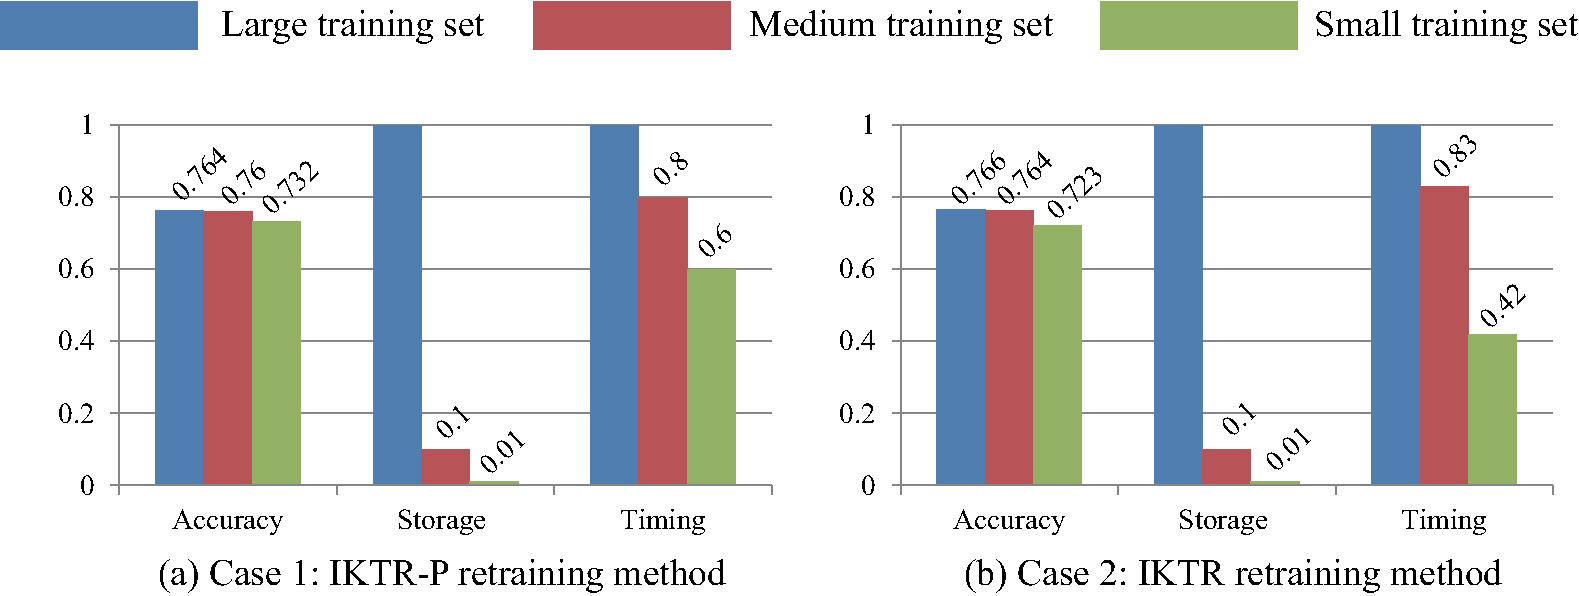
\includegraphics[width=0.75\linewidth]{images/OL-fig17}
    \caption{Trade-offs between the recovered model accuracy, storage and timing costs.}
    \label{fig:differenttrainingset}
    \vspace{-20pt}
\end{figure}

To further reduce the storage overhead of implementing the IKTR and IKTR-P algorithms on the edge device, we have made an analysis of using IKTR-P method for online model retraining with different sizes of training datasets. We conducted the experiments on SLC ReRAM and reached the same conclusion on MLC ReRAM. As shown in Fig. \ref{fig:differenttrainingset}, we randomly chose 500 (small), 5,000 (medium) and 50,000 (large) training samples from the original training set for faulty ConvNet retraining. It’s obvious that the memory consumptions are related to the size of training set. Using the small training dataset for model learning only costs {1\%} storage compared with using the large training dataset. However, fewer samples for training leads to limited accuracy improvement capacity. Using small training set for faulty model retraining causes about {4\%} accuracy loss on average, which is insufficient to meet the high accuracy requirement of deep-learning applications. In addition, we found that leveraging medium training set for  IKTR-based model retraining had quite small accuracy drop of up to {4\textperthousand} from using the large training set, but enables {90\%} storage saving as well as more than {17\%} training time reduction. %Specifically, the medium training set only needs 39.4MB back-up storage for storing the intermediate activations. 
Therefore, to achieve low storage costs with high retrieved model accuracy, it is recommended to use the medium training set for IKTR-based model faulty model retraining.


(d) Impact of the fault occurrence positions

\begin{figure*}
    \centering
    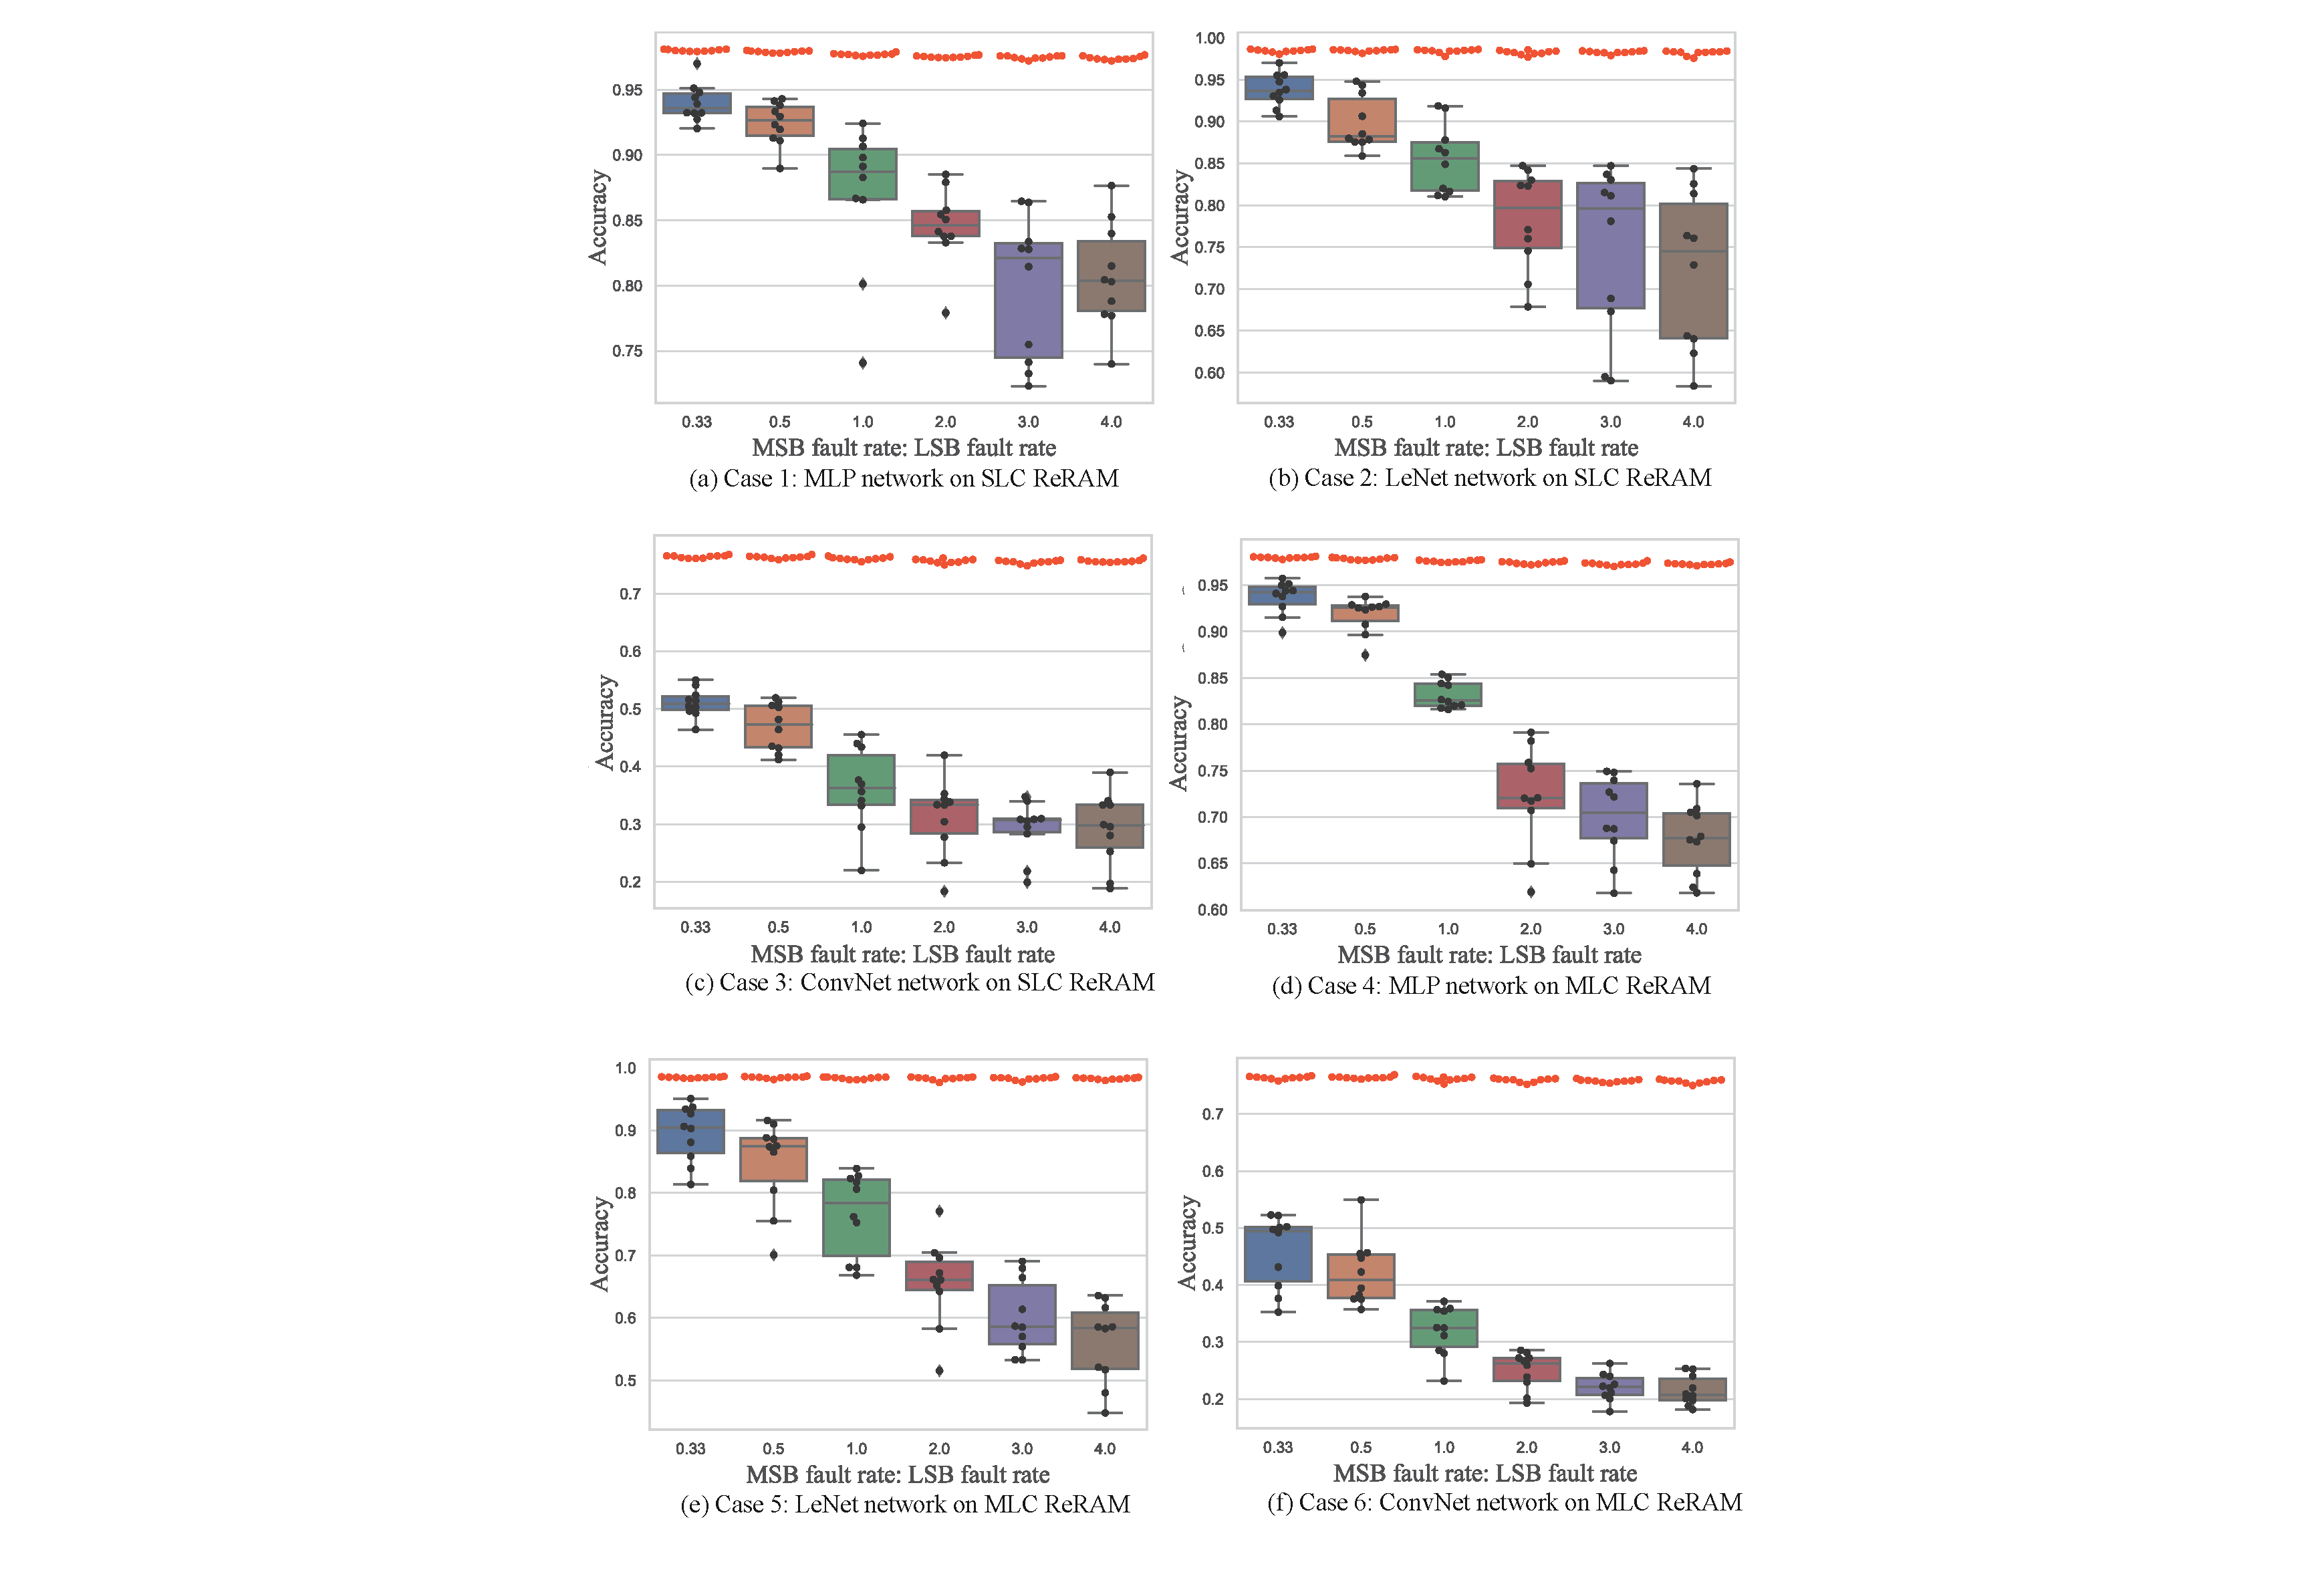
\includegraphics[width=0.85\linewidth]{images/OL-fig18}
    \caption{Impact of fault positions on model accuracy. The red dots presented the recovered model accuracy with IKTR-P method. The black dots presented the faulty model accuracy. Boxes show median and 2nd and 3rd quartile of the faulty model accuracy.}
    \label{fig:proportionalfaultinjectresult}
    \vspace{-10pt}
\end{figure*}

To evaluate the performance impact on the IKTR-based model retraining algorithm with different bit positions of the faults occurring in the neural network weights,  we have repeated the evaluations with our proposed IKTR-P method. For each benchmark, we randomly injected a fixed number of stuck-at faults and varied the proportion of faults that occurred in MSBs (Most significant bits) and LSBs (Least significant bits) of weight values. In addition, we tested ten faulty models for each fault occurrence scenario and simulated on both SLC and MLC ReRAMs. The experimental results are plotted in the Fig. \ref{fig:proportionalfaultinjectresult}. Several conclusions can be drawn as follows. First, even the fault rates are the same, the accuracies of faulty neural networks will be different according to the fault occurrence positions. As shown in Fig. \ref{fig:proportionalfaultinjectresult}, we varied the proportion of faults that occurred in MSBs vs. LSBs from 0.33 to 4 on all the three tested benchmarks. It is observed that when the fault rate of the MSBs is four times more than the fault rate of the LSBs, the average accuracy of faulty MLP networks significantly drops from {98\%} to {81\%} (Fig. \ref{fig:proportionalfaultinjectresult}(a)). Since the ConvNet is more sensitive to fault-induced weight variations, it is observed in Fig. \ref{fig:proportionalfaultinjectresult}(f) that, when {80\%} of the total injected faults occur in high-order positions, the average accuracy drops even more than 50\%. In contrast, when {67\%} of the injected faults occurr in LSBs of the weight values in ConvNet, the accuracy degradation is only {0.6\%} on average. This phenomenon can be explained by that faults in MSBs cause larger deviations in magnitude of weight values, increasing the possibility of a decrease in the accuracy of the neural network. Second, note that for all the tested benchmarks, the online remedy method IKTR-P can recover the deep learning system accuracy from up to {57\%} fault-induced accuracy degradation with less than {2\%} accuracy loss through fault-tolerant model retraining.

\subsection{Discussion}
In this paper, we comprehensively analyze the reliability issues of ReRAM-based edge neural accelerators and present RRAMedy, a novel framework to protect ReRAM chips from both permanent faults and soft faults. For fault detection, we introduce a lightweight Adversarial Example Testing method to detect the subtle fault-induced variations. For retrieving the system performance, according to the computing capacity and application scenarios of edge devices, we put forward an edge-cloud collaborative model retraining method and an in-situ model retraining algorithm. The experimental results show that the RRAMedy has high fault detection probability and can recover the recognition accuracy with little performance degradation.

\section{Summary}
To be added.

\bibliographystyle{plain}
\bibliography{refs}



